\ifdefined\luluflag
  \documentclass[12pt,twoside]{book}
\else
  \documentclass[12pt,oneside]{book}
\fi
\usepackage{graphicx}
\usepackage{makeidx}
\usepackage{tocloft}
\usepackage{relsize}
\usepackage{amsmath}
\usepackage{multicol}
\usepackage{colortbl}
\usepackage{ifpdf}
\usepackage{textcomp}

\ifpdf
  \ifdefined\luluflag
    \usepackage{fancyhdr}
    \pagestyle{fancy}
    \fancyhead{}
    \fancyhead[LE]{\slshape \nouppercase \leftmark}
    \fancyhead[RO]{\slshape \nouppercase \rightmark}
    \addtolength{\evensidemargin}{-8mm}
    \addtolength{\oddsidemargin}{8mm}
    \pdfpageattr{
    /MediaBox [0 0 621.00000 801.00000]
    /TrimBox [0.00000 9.00000 612.00000 792.00000]}
    \pdfminorversion=3
    \pdfcatalog{
    /OutputIntents [ <<
    /Info (none)
    /Type /OutputIntent
    /S /GTS_PDFX
    /OutputConditionIdentifier (lulu.com)
    /RegistryName (http://www.color.org/)
    >> ]
    }
  \fi
  \ifdefined\htmlflag
    \newcommand\myhref[2]{#2}
  \else
    \ifdefined\luluflag
      \usepackage[colorlinks=false]{hyperref}
    \else
      \usepackage[colorlinks=true,linkcolor=blue,urlcolor=red]{hyperref}
    \fi
    \newcommand\myhref[2]{\href{#1}{#2}}
  \fi
  \usepackage[toc,nopostdot,nonumberlist]{glossaries}
  \usepackage{ifthen}
  \graphicspath{ {../images/pdf/} }
  \usepackage[svgnames,table]{xcolor}
  \usepackage[tikz]{bclogo}
  \usepackage{hhline}
\else
  \usepackage[nopostdot,nonumberlist]{glossaries} %% with [toc] was appearing twice in TOC
  \usepackage[table]{xcolor}
  \usepackage{tex4ht}
  \newcommand\myhref[2]{\Link[#1 ID="1"]{}{}#2\EndLink}
  \graphicspath{ {../images/html/} }
  \renewcommand*{\glsgroupskip}{}% 
  \usepackage{wrapfig}
  \newenvironment{bclogo}[1][]{\medbreak\noindent\hangindent=2pc\hangafter=-2%
\ignorespaces%
\begin{wrapfigure}{l}{0.5\textwidth}
\includegraphics[]{warning}}%
{\end{wrapfigure}%
\medbreak\par\addvspace{\baselineskip}\bigskip\rule{1ex}{1ex}}
\fi

\usepackage{enumerate}
\usepackage{enumitem}
\usepackage[parfill]{parskip}
\usepackage{wrapfig}
\usepackage{booktabs}

\setcounter{secnumdepth}{4}
\setcounter{tocdepth}{2}

\makeatletter

\newcommand{\strong}[1]{\@strong{#1}}
\newcommand{\@@strong}[1]{\textbf{\let\@strong\@@@strong#1}}
\newcommand{\@@@strong}[1]{\textnormal{\let\@strong\@@strong#1}}
\let\@strong\@@strong

% Add a hair space if the fraction is followed by a non-space token.
\newcommand{\textfrac@kern}{%
  \ifx\textfrac@nexttoken\@sptoken%
    %
  \else%
    \kern.08333em%
  \fi%
}

% The non-star version of \textfrac uses a diagonal solidus.
\newcommand{\textfrac@nostar}[3][]{%
  \mbox{%
    \ifthenelse{\not\equal{#1}{}}%  Test for integer portion [optional #1]
      {#1\/\kern.05em}%                 Present? Emit integer and hair space
      {}%                             Not present? Emit nothing
    \raisebox{.775ex}{\tiny #2}%    Emit numerator [#2]
    \raisebox{.365ex}{\kern-.15em{\scriptsize /}\kern-.15em}%  Emit solidus
    \raisebox{0ex}{\tiny #3}%       Emit denominator [#3]
  }%
  \futurelet\textfrac@nexttoken\textfrac@kern%
}

% The star version of \textfrac uses a horizontal rule.
\newlength\textfrac@width@num%
\newlength\textfrac@width@denom%
\newlength\textfrac@width@%
\newcommand{\textfrac@star}[3][]{%
  \settowidth{\textfrac@width@num}{\tiny #2\/}%
  \settowidth{\textfrac@width@denom}{\tiny #3\/}%
  \ifthenelse{\lengthtest{\textfrac@width@num<\textfrac@width@denom}}%
    {\let\textfrac@width@\textfrac@width@denom}%
    {\let\textfrac@width@\textfrac@width@num}%
  \mbox{%
    \ifthenelse{\not\equal{#1}{}}%  Test for integer portion [optional #1]
      {#1\/\kern.08333em}%              Present? Emit integer and hair space
      {}%                             Not present? Emit nothing
    \ooalign{%
      \relax\cr%
      \noalign{\vskip-1.1ex}%
      {\hss\tiny #2\/\hss}\cr%        Emit numerator [#2]
      \noalign{\vskip1.1ex}%
      \rule[.6666ex]{\textfrac@width@}{.4pt}\cr%   Emit horizontal rule
      \noalign{\vskip.4ex}%
      {\hss\tiny #3\/\hss}\cr%        Emit denominator [#3]
      \noalign{\vskip-.4ex}%
    }%
  }%
  \let\textfrac@width\undefined%
  \futurelet\textfrac@nexttoken\textfrac@kern%
}

% Select between \textfrac and \textfrac*.
\def\textfrac{\@ifstar\textfrac@star\textfrac@nostar}

\makeatother

\ifpdf
\newcommand*{\titleTH}{\begingroup% T&H Typography
\clearpage
\thispagestyle{empty}
\raggedleft
\vspace*{\baselineskip}
{\Large\ \ }\\[0.167\textheight]
{\textcolor{Red}{\bfseries{\Huge S}{\LARGE AILFISH}}}\\[\baselineskip]
{\bfseries{\Large Reference Manual}}\\[\baselineskip]
{\small v7.7}\par
\vfill
{\Large Laurel Newman}\\[\baselineskip]
{\large \today}\par
\vspace*{3\baselineskip}
\endgroup}
\else
\newcommand*{\titleTH}{\maketitle}
\fi

\ifpdf
\newcommand\NextFile[1]{}
\fi

\renewcommand{\cftchapleader}{\cftdotfill{\cftdotsep}} % for chapters
\renewcommand{\cftsecleader}{\cftdotfill{\cftdotsep}} % for sections

\setlength{\parindent}{1.5em}

\makeindex

\makeglossaries

\def\secondpage{\clearpage\null\vfill
\thispagestyle{empty}
\begin{minipage}[b]{0.9\textwidth}
\ifpdf
  \footnotesize
\fi
\raggedright
Copyright \copyright\ 2014, Laurel Newman.
\newline
This work is licensed under the Creative Commons Attribution-ShareAlike 4.0
International License,
\myhref{http://creativecommons.org/licenses/by-sa/4.0/}{http://creativecommons.org/licenses/by-sa/4.0/}.\\
MakerBot and The Replicator are trademarks of MakerBot Industries, LLC.\\
Simplify3D is a trademark of Simplify3D LLC.\\
Kapton is a trademark of E.\,I. du Pont de Nemours and Company.
\end{minipage}
\vspace*{2\baselineskip}
\cleardoublepage}

\makeatletter
\g@addto@macro{\titleTH}{\secondpage}
\makeatother

\title{Sailfish Reference Manual}
\author{Laurel Newman}

\begin{document}

\titleTH

\frontmatter

\NextFile{toc.html}

\tableofcontents

\ifdefined\luluflag
\else
  \relsize{+1}
\fi

\newglossaryentry{EEPROM}
{
        name={EEPROM},
        description={Your printer contains a section of permanent memory
called ``EEPROM''.  The term ``EEPROM'' is an acronym for
Electrically Erasable Programmable Read-Only Memory.  This permanent
memory is used by the printer to store configuration and usage
information.  The printer's ``onboard parameters'', sometimes called
``onboard preferences'', are stored in its EEPROM.},
        sort=EEPROM
}

\newglossaryentry{FAT-16}
{
        name={FAT-16, FAT-32},
        text={FAT-16 or FAT-32},
        description={The SD cards used with your printer utilize a ``file system''
to organize the files on the card.  Sailfish supports two types of
file systems: FAT-16 and FAT-32.  All modern operating systems can set up
your SD card using either of those two file systems.  However, you may
not be given a choice of which to use: often FAT-16 is automatically
seleced for SD cards with 2~GB or less space and FAT-32 is used for
larger cards.},
        sort=FAT-16
}

%\newglossaryentry{FAT-32}
%{
%        name={FAT-32},
%        description={See \gls{FAT-16}.},
%        sort=FAT-32
%}

\newglossaryentry{Gen 3}
{
        name={Gen 3},
        description={The third generation of RepRap 3D printer electronics
was referred to as ``Gen 3'' electronics.  The MakerBot Cupcake uses this
generation of RepRap electronics.},
         sort=Gen 3
}

\newglossaryentry{Gen 4}
{
        name={Gen 4},
        description={The fourth generation of RepRap 3D printer electronics
was referred to as ``Gen 4'' electronics.  The MakerBot Thing-o-Matic uses this
generation of RepRap electronics.},
         sort=Gen 4
}

\newglossaryentry{HBP}
{
        name={HBP},
        description={Heated Build Platform.  Some printers include a
build platform which incorporates a heater to enable heating of the build
surface to a designated temperature.  Heating the build surface promotes
better adhesion and may, for some plastics, reduce warping.},
        sort=HBP
}

\newglossaryentry{home offset}
{
        name={Home offset},
        text={home offset},
        description={Each printer has three home offsets: the X, Y, and Z
home offsets.  Each value defines the printer's position along the associated
axis after homing to an endstop on that axis.  See
Section~\ref{sec:home-offsets} for further information.},
        plural={home offsets},
        sort=home offset
}

\newglossaryentry{Jetty Firmware}
{
        name={Jetty Firmware},
        description={The Sailfish firmware was originally named
``Jetty Firmware''. Originally based upon v3.1 of the G3Firmware from
MakerBot, the Jetty Firmware was first released in 2011 as v3.2.  (Note that
the G3Firmware from MakerBot applied to both Gen 3 and Gen 4 electronics.)
In early 2012, portions of Marlin were ported to MakerBots and incorporated
into the Jetty Firmware.  In October 2012, the Jetty Firmware was
renamed to Sailfish and released as Sailfish v4.0 for Thing-o-Matics and
Cupcakes and as v6.2 for Replicators.},
        sort=Jetty Firmware
}

\newglossaryentry{LCD}
{
        name={LCD},
        description={LCD is an acronym for ``Liquid Crystal Display''.  Many
3D printers include a LCD screen on their front and use it to display
information and as part of their interaction with users via an associated
keypad.},
        sort=LCD
}

\newglossaryentry{MightyBoard}
{
        name={MightyBoard},
        description={The MightyBoard is the name MakerBot gave to the
electronics in their Replicator 1 and 2 series of printers.  The Replicator 1
contains a MightyBoard revision E board (``rev E'').  The Replicator 2 contains
either a MightyBoard rev G or H board depending upon with which the printer was
manufactured.  The Replicator 2X contains a MightyBoard rev H.},
         sort=MightyBoard
}

\newglossaryentry{RPM gcode}
{
        name={RPM gcode},
        description={Early ``do-it-yourself'' 3D printers used DC
motors for extrusion.  The desired rate of extrusion was achieved by
setting the ``rotations per minute'' (RPM) of the motor.  The gcode
for this style of 3D printing is referred to as ``RPM gcode''.  Cupcakes
and early Thing-o-Matics used DC motors for extrusion.},
        sort=RPM gcode
}

\newglossaryentry{S3G}
{
        name={S3G},
        description={S3G is an acronymn for ``Sanguino3 Gcode'' and is a
3D printer control language.  Files containing S3G use the file extension
\texttt{.s3g}.  See Section~\ref{sec:s3g-x3g} for further information.},
        plural={\texttt{.s3g}},
        sort=S3G
}

\newglossaryentry{SD card}
{
        name={SD card},
        description={An SD card is specific type of memory flash card and is
used to convey print files to your printer without using a USB or network
connection.  SD cards come in a variety of sizes, ranging from a fraction of
a gigabyte to upwards of 256 gigabytes or more.   Sailfish supports SDSC
(standard capacity), SDHC (high capacity), and SDXC (extended capacity) SD
cards.  The term ``SD'' is an acronym for ``Secure Digital''.},
        plural={SD cards},
        sort=SD card
}

\newglossaryentry{toolhead offset}
{
        name={Toolhead offset},
        text={toolhead offset},
        description={The ``toolhead offset'' is the physical spacing between
two extruder nozzles.  See Section~\ref{sec:toolheadoffsets} for further
information.},
        plural={toolhead offsets},
        sort=toolhead offset
}

\newglossaryentry{Volumetric 5D gcode}
{
        name={Volumetric 5D gcode},
        description={The use of DC motors and RPM gcode was replaced
by discrete stepper motors and ``Volumetric 5D'' gcode.  Volumetric gcode
sought to specify the volume of plastic to be extruded rather than the
``flowrate'' of plastic as controlled by a DC motor's rotational speed.
Moreover, the new motion commands used five parameters: four spatial
parameters X, Y, Z, and E (extruder), and a fifth speed parameter, feedrate.
The use of five parameters led to the name ``5D''.  The combination of
these two changes led to the name ``Volumetric 5D''.},
        sort=Volumetric 5D gcode
}

\newglossaryentry{X3G}
{
        name={X3G},
        description={X3G is an extended form of \gls{S3G} containing accelerated
motion commands. Files containing X3G use the file extension \texttt{.x3g}.
See Section~\ref{sec:s3g-x3g} for further information.},
        plural={\texttt{.x3g}},
        sort=X3G
}

\newglossaryentry{firmware}
{
        name={Firmware},
        text={firmware},
        description={Firmware is the software that is embedded in hardware
and used to control the operation of the hardware.},
        sort=firmware
}

\newglossaryentry{gcode}
{
        name={Gcode},
        text={gcode},
        description={Gcode, sometimes written as ``G-code'', is a numerical control programming language used
to control the operation of machine tools such as 3D printers.  While there is an international standard
for gcode, the 3D printing community loosely adheres to it.  For example,
different 3D printers accept different variations of gcode.  MakerBot
printers do not even directly accept gcode and instead consume a binary
language known as S3G.  The specific gcodes produced by different
slicers and accepted by different printers are often not well specified.},
        sort=gcode
}

\newglossaryentry{mcode}
{
        name={Mcode},
        text={mcode},
        description={Gcode can contain ``miscellaneous'' function codes
known as ``mcodes'' and which begin with the letter ``M''.  See \gls{gcode}
for information on gcode.},
        sort=mcode
}

\newglossaryentry{onboard parameters}
{
        name={Onboard parameters},
        text={Onboard Parameters},
        description={Many 3D printers store within their microprocessor
configuration parameters which may be read and changed by users.  As these
parameters live within the printer, they are referred to as ``onboard
parameters''.  They are typically stored in the printer's EEPROM.},
        sort=onboard parameters
}

\newglossaryentry{slicer}
{
        name={Slicer},
        text={slicer},
        description={The process of turning a 3D model into printing
instructions --- gcode --- is referred to as ``slicing''.  That name
derives from the fact that the process takes slices of the model
and determines the necessary ``tool paths'' (extruder paths) to print
that slice.  The slice is a ``layer'' of the print.  As the process
is referred to as slicing, the software which implements the process
is often called a ``slicer''.},
        sort={slicer},
        plural=slicers
}

\newglossaryentry{tool}
{
        name={Tool},
        text={tool},
        description={In gcode parlance, an extruder is a ``tool''
which is controlled by the printer.  That is, a ``tool'' is another name for
an extruder.  If your printer has a single extruder, than that extruder
may be referred to as ``tool 0''.  If your printer has two extruders,
then the right extruder is ``tool 0'' and the left extruder is ``tool 1''.
To further confuse matters, in gcode motion commands for the right
extruder may use the prefix ``A'' while the left extruder the prefix ``B''.},
        sort=tool
}

\newglossaryentry{corner ringing}
{
        name={Corner ringing},
        text={corner ringing},
        description={This is a type of print defect characterized by a ripple pattern which
quickly dampens and is seen on the vertical faces of prints, particularly
after a direction change in the surface.},
        sort=corner ringing
}

\newglossaryentry{telegraphing}
{
        name={Telegraphing},
        text={telegraphing},
        description={A print defect caused by too thin of an exterior
shell through which interior printing penetrates leaving visible surface
blemishes.},
        sort=telegraphing
}

\newglossaryentry{over-extrusion}
{
        name={Over-extrusion},
        text={over-extrusion},
        description={When the extruder outputs a surplus of plastic,
o\-ver-ex\-tru\-sion results.  Over and under-extrusion are caused by a mismatch
between the slicer's expectations and reality: the slicer expects that when
a millimeter of raw filament is fed into the extruder, a specific volume
$V_e$ of plastic will then be extruded --- output by the extruder.  When
the actual volume of plastic output, $V_a$, exceeds $V_e$, over-extrusion
results; when $V_a$ is less than $V_e$, under-extrusion results.  There are
a number of causes of this mismatch, but it generally is the result of the
input filament diameter not matching what the slicer expected, or the
steps per mm for the extruder being incorrect.  By first calibrating your
slicing profile as per Section~\ref{sec:cube} for each type of plastic, and
then always measuring your filament diameter, you can prevent over and
under-extrusion from occurring.},
       sort=over-extrusion
}

\newglossaryentry{under-extrusion}
{
        name={Under-extrusion},
        text={under-extrusion},
        description={When the extruder outputs a deficit of plastic,
under-extrusion results. See \gls{over-extrusion}.},
       sort=under-extrusion
}

\newglossaryentry{slicing profile}
{
        name={Slicing profile},
        text={slicing profile},
        description={Most slicers have a mechanism whereby you collect
together a number of configuration settings used by that slicer when
preparing a model for printing.  Such a collection of settings is here
referred to as a ``slicing profile''.  A given slicer may use a different
name (e.g., a ``factory'' in Simplify3D).},
        plural={slicing profiles},
        sort=slicing profile
}

\newglossaryentry{dualstrusion}
{
        name={Dualstrusion},
        text={dualstrusion},
        description={Making a 3D print using two extruders --- dual extrusion
--- is sometimes referred to ``dualstrusion''.  The term was coined by
MakerBot when they first began experimenting with dual extrusion for
their Thing-o-Matic printer.},
      sort=dualstrusion
}

\newglossaryentry{raft}
{
        name={Raft},
        text={raft},
        description={To promote better build plate adhesion or to accommodate an uneven build surface, most slicers can add to your print a thick series of layers which can later be removed once the print is finished.  These layers --- referred to as a raft --- are printed slowly so as to promote better adhesion to the build plate as well as to level out the printing surface.},
        sort=raft
}

\newglossaryentry{deprime}
{
        name={Deprime},
        text={deprime},
        description={An extruder is ``primed'' by feeding filament into the extruder.  Conversely, it is ``deprimed'' by pulling or retracting the filament from the extruder.  Depriming an extruder serves to reduce the pressure within the extruder.  This in turn helps reduce the amount of unwanted plastic which oozes out of the extruder, particularly when no extrusion is desired such as during a printing pause or a ``travel move''.},
        sort=deprime
}

\newglossaryentry{travel move}
{
        name={Travel move},
        text={travel move},
        description={When printing, there are two types of motions or moves: an extrusion move in which extrusion of plastic occurs, and a travel move in which motion occurs absent extrusion.  Travel moves serve to transfer the extruder to another portion of the print, without printing any plastic.},
        sort = {travel move}
}

\newglossaryentry{GPX}
{
        name={GPX},
        description={GPX is software used to convert gcode to S3G/X3G for use with a
MakerBot style printer.  GPX may be found at Thingiverse as \myhref{http://www.thingiverse.com/thing:81425}{Thing \#81425}.},
        sort=GPX
}

\newglossaryentry{shell}
{
        name={Shell},
        text={shell},
        description={When a model is prepared for printing by a slicer, the slicer generates commands to print a solid exterior.  The exterior is typically printed by following the model's perimeter.  The perimeter may be printed multiple times per layer, each time inset from the prior pass.  The final result can be thought of as a series of nested shells, one inside the other, from which arises the term ``shell''.  With some slicers, you control the thickness of the solid exterior by specifying the number of shells to generate.},
        sort=shell
}

\newglossaryentry{infill}
{
        name={Infill},
        text={infill},
        description={Each model to be printed is comprised of an exterior and an interior.  While the exterior is typically printed solid with no holes or gaps, the interior may range anywhere from completely empty to completely solid. The plastic printed in the interior is known as ``infill'' and its solidity is the ``infill percentage''.  For example, 0\% infill means the print is completely hollow and 100\% infill means it is fully solid.  Printing time is reduced and plastic is saved by printing with infill percentages significantly less than 100\%.  The amount of infill you should use depends upon the nature of the piece being printed and its intended usage.},
        sort=infill
}

\newglossaryentry{heatsink cooling fan}
{
        name={Heatsink cooling fan},
        text={heatsink cooling fan},
        description={Many MakerBot-style 3D printers include, for each extruder, a heatsink which helps cool portions of the extruder.  This heatsink often includes a fan mounted to the heatsink and which helps move air past the heatsink's cooling fins.},
        sort={heatsink cooling fan},
        plural=heatsink cooling fans
}

\newglossaryentry{print cooling fan}
{
        name={Print cooling fan},
        text={print cooling fan},
        description={Some plastics such as PLA take longer to cool after extrusion.  This can be significant when printing small models for which there is insufficient time for a layer to cool before the next layer is printed.  Additional air flow directed at the print can speed up cooling.  For this reason, some printers are equipped with a ``print cooling fan''.},
        sort={print cooling fan},
        plural={print cooling fans}
}

{
\ifdefined\luluflag
\else
  \relsize{-1}
\fi
\ifdefined\luluflag
\fancyhead{}
\fi

\NextFile{acknowledgements.html}

\chapter{Acknowledgments}

%{\Huge\textbf{Acknowledgments}}
%\addcontentsline{toc}{chapter}{Acknowledgments}

Portions of this documentation were adapted from earlier works by Jetty and Dan Newman.  Special thanks to Ryan Carlyle for providing editing assistance; Mr.~Carlyle's expertise is greatly appreciated.  And further thanks are due to these companies and individuals for their generous contributions, which made the production of this documentation possible.

\noindent Corporations:

\begin{description}
\item[] \textbf{Magicfirm Europe AB}, Makers of the ZYYX 3D Printer,
\ifpdf\newline\fi
\myhref{http://zyyx3dprinter.com/}{http://zyyx3dprinter.com/}
\item[] \textbf{RAFFLE} (Carl Raffle), Maker of 3D printers, components and upgrade parts,
\myhref{http://shop.raffle.ch/}{http://shop.raffle.ch/}
\end{description}

\noindent Individuals:

{
\ifpdf
\setlist[description]{parsep=0pt}
\begin{multicols}{2}
\fi
\begin{description}
\item[] Guido Alphen
\item[] Ted B{\"a}ckman
\item[] Federico Boldori
\item[] Scott Booker
\item[] Jake Bordens
\item[] Joseph Brunson
\item[] Perry Cain
\item[] Chris Chavez
\item[] Joseph Chiu
\item[] Gary Crowell
\item[] Scott Davies
\item[] Ward Elder
\item[] EmbeddedJunkie, \ifpdf\newline\indent\fi aka Juan Gutierrez
\item[] Mike Hellers
\item[] Clinton Hoines
\item[] Anna Kaziunas France
\item[] David Lancaster
\item[] Christopher Matthes
\item[] Erik Mendoza
\item[] Laird Popkin
\item[] Fred Stahmer
\item[] Gregory Sullivan
\item[] Richard Webb
\item[] Scott Wells
\item[] Bradley Wong
\item[]
\end{description}
\ifpdf
\end{multicols}
\fi
}

\clearpage

\ifdefined\luluflag
\fancyhead[LE]{\slshape \leftmark}
\fancyhead[RO]{\slshape \rightmark}
\fi

}

\mainmatter

\NextFile{introduction.html}
\chapter{Introduction}

Sailfish began as enhanced control software for MakerBot printers,
incorporating new features intended for advanced users.  With its numerous
features, Sailfish has evolved into the firmware of choice for users of MakerBot-style printers based upon the Replicator 1 and 2 series
of 3D printers as well as the earlier Thing-o-Matic and Cupcake lines.

A 3D printer's firmware is the software which resides within the
printer and controls the printer's behavior. It is the software which
receives printing instructions from MakerWare, ReplicatorG, SD card
files, and other desktop programs and then executes them to create
your 3D print.

This documentation is intended to help you navigate the firmware on your printer, from basic setup and navigation of the \gls{LCD} screen, to advanced adjustments, updates, and the particulars of diagnosing Sailfish-specific issues.  The most recent documentation of Sailfish may be found online at:
\begin{quote}
\myhref{http://www.sailfishfirmware.com}{http://www.sailfishfirmware.com}
\end{quote}

\begin{bclogo}[logo=\bcinfo, noborder=true, couleurBarre=yellow]{Note}
Consult the documentation supplied with your printer for general printing instructions.  The \emph{Sailfish Reference Manual} only provides detailed information on the use of the Sailfish \gls{firmware} and is not intended to replace your printer's documentation.  
\end{bclogo}

\pagebreak[4]

Suggested starting points in the documentation are:
\begin{itemize}
\item Chapter~\ref{chap:basic_usage}, Basic Usage: introductory information for new 3D printer operators.
\item Chapter~\ref{chap:whatever}, Front Panel Operation: users who are familiar with 3D printers, but new to Sailfish, can begin here.
\item Chapter~\ref{chap:install}, Installing Sailfish: if you are seeking information on installing Sailfish, start here.
\end{itemize}

The Sailfish firmware is open source and builds upon earlier firmwares such as Gen~4, Grbl, and Marlin.  MakerBot's own firmware for Replicators incorporates the core of Sailfish.  Source code for Sailfish is available for inspection and download at\index{Source code}

\begin{description}
\item[] \textbf{Replicators}\
\newline
\myhref{https://github.com/jetty840/Sailfish-MightyBoardFirmware}{https://github.com/jetty840/Sailfish-MightyBoardFirmware}
\item[] \textbf{Thing-o-Matics, Cupcakes}\newline
\myhref{https://github.com/jetty840/Sailfish-G3Firmware}{https://github.com/jetty840/Sailfish-G3Firmware}
\end{description}

\noindent Important information about the compiler and tools required if you wish to build Sailfish yourself is located in the respective \texttt{doc/} directories in the \texttt{avr-gcc.markdown} file.


\NextFile{basic-usage.html}

\chapter{Basic Usage} \label{chap:basic_usage}

This chapter is intended to provide new printer owners with basic information pertaining to the initial setup of their printer in order to help them familiarize themselves with their printer and accomplish a first print.  The information here is a supplement to the documentation which accompanied your printer --- the information specific to your make and model of 3D printer.

\NextFile{basic-usage-leveling.html}

\section{Leveling the Build Plate} \label{sec:leveling}
\index{Tramming|see {Leveling}}
\index{Leveling|(}

The first step towards ensuring the success of a 3D print is making certain that the build plate --- the surface atop which the 3D print is printed --- is well ``trammed'' to the extruder nozzle.  Despite the fact that this process is commonly referred to as ``leveling'', you should not \emph{use} a level as you are not leveling the plate to the horizon.  In actuality, you are making sure that the top surface of the build plate is parallel to the plane the extruder nozzle travels in.  While machinists call this ``tramming'', in the world of 3D printing this is called ``leveling''.

\begin{bclogo}[logo=\bcattention, noborder=true, couleurBarre=red]{Important}
If your printer features auto-leveling or assisted-leveling, then consult the directions for your printer to check whether or not you should manually level the build plate.  It is strongly advised that you follow your printer's specific directions for initial setup.  Often, printers with these features arrive already leveled and merely require some printer specific ``first run'' checks.
\end{bclogo}

Before beginning:

\begin{enumerate}
\item Check your printer's documentation to determine where the build plate's leveling adjustments are.  Most printers have either three or four leveling adjustments.
\item Once the leveling adjustments are identified, determine how to adjust them to raise and lower the plate.  A common form of adjustment is a threaded stud with thumbnut.  If you are looking down towards the top of the plate, you then turn the thumbnut clockwise to raise the plate and counterclockwise to lower the plate.
\item Find a sheet of paper to use as a ``feeler gauge''.  You will use this to set a consistently small gap between the tip of the extruder nozzle and the top of the build plate.  \Glspl{slicer} typically assume this gap to be about 0.1~mm --- approximately the thickness of a sheet of paper.  If you have actual automotive or machinist's feeler gauges, then use such a gauge instead.
\item If your build plate requires a surface treatment (such as tape) which is not already applied, then apply it now before leveling.  Some build plates, such as those provided with ZYYX printers, do not require any treatment.  Most build plates have an aluminum or glass surface that requires a treatment of Kapton (polyimide) tape for ABS or blue ``painter's'' tape for PLA.  Often, these plates come shipped with tape already applied.  Like your filament, the tape is a ``consumable'' and will need to be replaced in time.  Note that if your plate requires a treatment but is shipped without one, then you need to decide with what type of plastic you will be printing.  If you will not be using ABS or PLA, consult the directions that came with your printer.
\end{enumerate}

To level your build plate for the first time, the procedure is as follows.  Again, note that you should consult the documentation that accompanied your printer to check for printer-specific instructions, as the following instructions are generic by necessity:

\begin{enumerate}
\item Adjust the leveling points in order to lower your build plate relative to its support mechanism (e.g., support arms).  This does not mean you should lower the entire assembly down the Z rods.  Rather, compress the springs on which the build plate rides and tighten the thumbnuts, thereby lowering the plate itself in relation to the arms and other structures supporting it.  This ensures that there is a significant gap between the nozzle and the build plate's surface in order to reduce the risk of damaging either.
\item Remove any debris from the tips of the extruder nozzles.  If there is a small bead of plastic, it can be broken off with small tweezers.
\item Turn on the printer.
\item From the main menu (Section \ref{sec:Main}) of your LCD display, select the ``Utilities'' menu (Section \ref{sec:utilities}) by pressing the down key twice and then pressing the center key.  The keypad and the LCD screen are normally located close to each other somewhere on the front of the printer.
\item Within the Utilities menu, press the down key to scroll downwards until you have selected the ``Home Axes'' item (Section~\ref{sec:home-axes}).  Press the center key to choose the item.
\item Having selected ``Home Axes'', the printer will move the extruders to the back, right corner.  Then the printer will raise the build platform twice, slowly the second time.
\item Once this homing operation is completed, manually slide the extruder assembly over the build surface, ensuring that it does not touch the top of the build surface anywhere.  If it does, then continue to lower the build surface using the leveling adjustments.  If the build surface cannot be lowered further and the extruder is still hitting it, either the Z endstop\footnote{The Z endstop is typically a limit switch which, when triggered, stops further upward motion of the build plate.  Consult your printer manual for information on the location and adjustment of this endstop.} may need to be lowered or a shim should be installed, after which Steps~5, 6, and 7 should be repeated.
\item Before beginning leveling, you need to heat up the build plate if you will be printing with it heated.  As some heated build surfaces expand a small amount or may even ``crown'' upwards in the middle a little when heated, the plate must be leveled in its operational configuration.  From the keypad press the left key to return to the main menu, then scroll up using the up key and select the Preheat item by pressing the center key, Section~\ref{sec:preheat}.  Make sure you are not heating the extruders by scrolling to their lines and pressing the center key to toggle the value to ``OFF''.  Likewise, ensure that the heating platform reads ``ON'' before scrolling up to the first line and pressing the center key to begin preheating.  A monitor screen will appear, similar to the one shown in Figure \ref{fig:tempform}.  Wait until the platform reaches its target temperature, which is usually 100\textdegree\,C for ABS or 50\textdegree\,C for PLA; the temperatures are displayed in the form current temperature/target temperature in degrees Celsius.  Once the platform is fully heated, press the left key to return to the main menu.

\begin{figure}[!htbp]
  \centering
    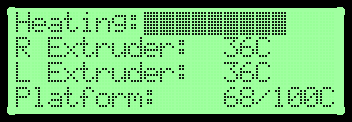
\includegraphics[]{preheat-monitor-01}
    \caption{Monitor Screen}
  \label{fig:tempform}
\end{figure}

\item From the Utilities menu, scroll down until you reach ``Level Build Plate'', then select it using the center key, Section~\ref{sec:levelbp}.
\item The printer will now home its axes as before, then move the nozzle to the approximate center of the build plate.  Directions will appear on the LCD screen; press the center key to advance from screen to screen.  The final screen will be the one depicted in Figure \ref{fig:level-01}.

\begin{figure}[!htbp]
  \centering
    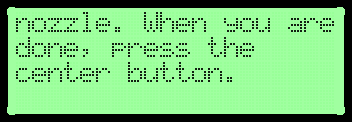
\includegraphics[]{level-01}
    \caption{Leveling}
  \label{fig:level-01}
\end{figure}

\item To level the build plate, manually move the extruder so that the nozzle is roughly over one of the adjustment points.  Take care to avoid dragging the nozzle across the build surface, as that may cause damage.  Then, adjust the point so that there is only a small gap between the tip of the nozzle and the top of the build surface.  Place the piece of paper between the two as you adjust.  You want to be able to slide the paper back and forth, but with some friction.
\item After you are satisfied that this point is adjusted, move the extruder to the next point to repeat the process.  Do not press the center key yet.
\item Once you have finished adjusting all the points, recheck them.  You may also wish to check the center of the build plate.  The plate may crown a little when heated and the long X rods supporting the extruder can sag a tiny amount.  As such, you may find the gap to be too small at the center.  If so, you may need to fiddle with the adjustment points until a more uniform gap across the plate is achieved.\footnote{For small, centered prints, having a 0.1~mm gap near the plate's center is critical and a slightly larger gap at the edges can be tolerated.  However, when doing large prints, it may be necessary to print with a \gls{raft} or to obtain a flatter build surface.  See your slicer's documentation for information on generating rafts.}  Note that turning all thumbnuts by an equal amount will raise or lower the entire plate evenly.
\item If you have finished checking and rechecking all your test points, and you are satisfied that the plate is level, then press the center key.  Now that you have completed leveling, you are ready to load filament.
\end{enumerate}

\begin{bclogo}[logo=\bcinfo, noborder=true, couleurBarre=yellow]{Note}
In general, you do not need to level your build plate before every print.  As you continue to use your printer, the frequency with which you need to level your plate will diminish.  However, in the first week or so you may need to level it every few prints.  This is in part due to your lack of experience, but may also
be the result of your printer settling in.
\end{bclogo}
\index{Leveling|)}

\NextFile{basic-usage-filament-loading.html}

\section{Loading Filament}
\index{Filament!Loading|(}

Before starting your first print, you must first load filament into each extruder you will be using.  However, even if your printer has two extruders, it is strongly recommended that you start with a simple print which uses only a single extruder --- preferably the right extruder.  As such, you should not load filament into the second extruder until you actually need to use it.

Most 3D printers come with a spool or two of filament, which is generally either ABS or PLA plastic.  While the loading directions are the same regardless, you should load a filament compatible with the treatment applied to the surface of your build plate (e.g., ABS for Kapton tape on the build surface; PLA for painter's tape on the build surface).

From the documentation for your printer, you will need to determine:

\begin{enumerate}
\item The proper filament spool mounting technique.  Many printers come with a rear-mounted filament spool.
\item The spool orientation and filament feed path.  It is important to set this up properly so as to prevent filament tangles and other feed-related problems.
\item The mechanical steps to load filament into your extruder's feed mechanism, as this varies between printers.
\end{enumerate}

Once you have determined the above information, you are ready to load filament into your extruder --- the righthand extruder if you have two:

\begin{enumerate}
\item With a pair of scissors, neatly trim the end of the filament.  Mount the filament spool in its correct orientation and feed the filament through any guide tubes along its feed path.  Do not yet attempt to load the filament into the extruder itself.
\item Turn on your printer.  Then, from the front LCD panel navigate with the down key to the ``Utilities'' item, Section \ref{sec:utilities}.  Press the center key to select it.
\item Within the Utilities menu, navigate to the line reading ``Filament Loading'' (Section~\ref{sec:filload}).  Again, press the center key to select this.
\item If your printer arrived with a short length of filament already loaded into the extruder, then you will want to unload it first:
\begin{enumerate}
\item Select ``Unload Filament'' and the printer will heat up the extruder to the temperature set in Preheat Settings under the Utilities menu, Section~\ref{sec:preheatset}.  By default, this is 230\textdegree\,C.  If you have two extruders, select this for the right extruder.
\item Once heated up, the printer will then begin to unload the filament.  After a few moments you should be able to manually pull the segment out.  This should \emph{not} require much force.
\item You may press the center key to stop the unloading process.
\end{enumerate}
\item Now select ``Load Filament''.  If you have two extruders, select loading
for the right extruder.
\item The printer will now begin to heat up the extruder to the temperature set in Preheat Settings under the Utilities menu.
\item Once the extruder has reached temperature, the front LCD panel will generate a screen telling you to begin loading the filament into the extruder.  The feed motor for the extruder will begin turning to allow you to load the filament.  Following the necessary procedure for your printer, load the filament into the extruder and allow it to feed the filament.
\item After a few moments, a hot plastic thread will begin to emerge from the extruder's nozzle.  If it is not initially the color of the filament you loaded, note that the factory may have tested the printer using a different color filament.  Allow the filament to extrude for at least 30 seconds before pressing the center key to stop the process.  Press the left key once to return to the Utilities menu; press the left key a second time to return to the top-level menu.
\end{enumerate}

\begin{bclogo}[logo=\bcinfo, noborder=true, couleurBarre=yellow]{Note}
If the extruded filament tends to curl upwards as it exits the nozzle, then there may be debris clogging the nozzle.  If such is the case, contact your printer manufacturer for assistance.  Also, if the extruded filament bubbles and pops a little, then your filament has absorbed too much moisture and may need to be dried out.  The proper way of drying it depends on the type of filament; contact your filament vendor for guidance.
\end{bclogo}

\index{Filament!Loading|)}

\NextFile{basic-usage-starting-a-print.html}

\section{Starting a Print}

\begin{bclogo}[logo=\bcattention, noborder=true, couleurBarre=red]{Important}
Do not leave your printer operating unattended!  Unless your printer manufacturer expressly states that your printer supports unattended operation, you must not allow it to operate unsupervised.  There have been cases of 3D printers failing and burning themselves down.  Unattended printing carries significant risk to life and property.  Be Safe!
\end{bclogo}

Most printers ship with an \gls{SD card} containing sample prints.  For your first print choose a sample that only requires the use of a single extruder.  If such a card was not supplied, then you will need to obtain a model and prepare it for printing with a \gls{slicer}.  Explaining this procedure is outside the scope of this document due to the numerous variables arising from printer, slicer, etc.\ variations.

Insert the SD card into the printer's SD card slot, and then turn on the printer.  From the main menu of the LCD screen select the ``Print From SD'' option, select the file you wish to print --- note that, if there are more than four files on the SD card, you may have to scroll down --- and then the print will begin.\footnote{For more details on navigating the ``Print From SD'' menu, finding hidden files, and making your files accessible see Section \ref{sec:sdmenu}.}  The print monitor screen will be generated; for more details see Section \ref{sec:printmon}.

\NextFile{basic-usage-tips.html}

\section{Tips}

Now that you have completed a print or two, here is further advice to help ensure your continued success.  Moving forward, keep in mind
that the most common problem people experience is getting the first layer
of their print to adhere properly to the build plate.  Here are some tips
which may prove helpful:

\begin{enumerate}
\item Properly leveling your build plate is critical to successful
printing.  Also, be consistent: use the same sort of paper each time or a
0.1~mm feeler gauge.  \emph{Do not eyeball the gap.}
\item Start with 0.30~mm layer height prints.  The lower the layer height, the
more important it is to have properly leveled the build plate as well as having a very flat
(non warped) build plate.  As you continue to print, you will get better
at leveling the plate, at which point you can try your hand at 0.20 and even 0.15 or
0.10~mm layer heights.  However, stick with 0.30~mm prints until you are experienced and reasonably skilled.
\item Use the proper build surface treatment.  Some printers such as MBot3D
and ZYYX come with a special build surface that requires no tape. Many other
printers, however, come with just an aluminum or glass plate.  For those
surfaces you need to add tape --- and not just any tape.  Use Kapton tape
(polyimide) for ABS prints and blue ``painter's'' tape for PLA.  Occasionally
wipe down the Kapton with acetone or the painter's tape with alcohol.  ABS
also requires a heated build plate to adhere well.
\item The ideal extrusion temperature for each filament type may differ.  While you should begin with the printer manufacturer's recommendations, you may wish to experiment some with higher or lower temperatures in order to find the optimum temperatures.
\end{enumerate}

\NextFile{basic-usage-next-steps.html}

\section{Next Steps}

Enjoy your printer!

Early on, you should perform basic printer calibrations.  For guidance, see Chapter~\ref{chap:tuning}.

Visit \myhref{http://thingiverse.com/}{Thingiverse} for an astounding
collection of printable models.  When you find a model you want to
print, check to see if there is advice for slicer settings.  Such information
is often found in the description or instruction sections of the
Thingiverse page for the model.  Gravitate towards models which have
actual pictures of the printed item as some models posted will not print easily --- or at all.  Seeing a photo of an actual print provides extra assurance that the model is sound.

After you have used your printer and slicer for a few weeks, branch
out and look at some other slicers.  Each slicer has
its own strengths and weaknesses.  Many of the slicers are under
active development, receiving new improvements regularly.  Keep in
mind, however, that MakerBot-style printers consume a format called
X3G (Section~\ref{sec:s3g-x3g}).  The gcode from your slicer is
converted to that format for you.  As of this writing, the slicers
which automatically perform this conversion for you are MakerBot
Desktop, MakerBot MakerWare, ReplicatorG -- Sailfish, and
Simplify3D.\footnote{Active development of Skeinforge, the slicer within
ReplicatorG, ceased in April 2012.}
While you can use other slicers such as Cura, KISSlicer, and slic3r,
you will need to use a tool to convert their gcode to X3G.  The
two common approaches are to either import the gcode into a slicer which
handles X3G or to use the \gls{GPX} tool to do the conversion.  GPX may be
found at Thingiverse as
\myhref{http://www.thingiverse.com/thing:81425}{Thing \#81425}.\index{GPX}

Finally, search out any user groups for your brand of printer.  Some
manufacturers run or link to online forums from their own web pages.
Other printer groups may be found at sites such as
\myhref{http://groups.google.com}{groups.google.com}.


\NextFile{ui.html}

\chapter{Front Panel Operation}\label{chap:whatever}

Since 2012, MakerBot printers and their clones have included a built in user
interface comprised of a \gls{LCD} screen and a five-button keypad.  With this
user interface, the printer can be operated without the use of a computer.

This chapter describes the operation of Replicator-style printers through this
built-in interface.

For users of Thing-o-Matics with ``Gen 4 LCD interfaces'', please refer
to the ``Pages Archive'' of the MakerBot Wiki found at
\myhref{http://www.makerbot.com/support/archive/}{http://www.makerbot.com/support/archive/}.  There, documentation for the Thing-o-Matic
LCD interface may be found as part of the ``\gls{Jetty Firmware}''
documentation.

\NextFile{ui-splash.html}

\section{Splash Screen}\label{sec:Splash}
\index{Screens!Splash}

Every time you power on your printer, the \gls{LCD} screen should be similar to the one pictured in Figure~\ref{fig:splash}.  This splash screen only lasts for a few seconds, so you may miss seeing it.

\begin{figure}[!htbp]
  \centering
    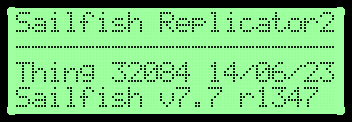
\includegraphics[]{splash-01}
    \caption{Splash Screen}
  \label{fig:splash}
\end{figure}

If, however, you should instead see a screen with two horizontal black bars (as pictured in Figure~\ref{fig:error}), then your printer either does not have \gls{firmware} loaded or has an electrical problem.\index{LCD!Solid bars}

\begin{figure}[!htbp]
  \centering
    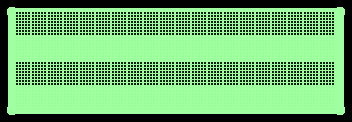
\includegraphics[]{splash-02}
    \caption{Bad News}
  \label{fig:error}
\end{figure}

The splash screen contains the following information:

\begin{enumerate}
\item The \myhref{http://www.thingiverse.com/thing:32084}{Thingiverse ``Thing'' number 32084}.
\item The date the firmware was built in year/month/day format.
\item The version and revision numbers.
\end{enumerate}

If you miss seeing the splash screen, this information may also be found in the ``Version Information'' item under the ``Utilities'' menu, Section~\ref{sec:versinf}.

After a few seconds, the splash screen is dismissed and replaced by the main
\ifpdf
menu.
\else
menu, Section~\ref{sec:Main}.
\fi

\NextFile{ui-main-menu.html}

\section{Main Menu}\label{sec:Main}
\index{Menus!Main}

The main menu (Figure~\ref{fig:main}) is your base of operations.  When it appears, the screen should have a title line displaying the name of the printer; you may change this name with either ReplicatorG or MakerWare.  The next three lines allow you to print from a memory card (i.e., an \gls{SD card}), preheat your printer, and access the printer's utilities.  

\begin{figure}[!htbp]
  \centering
    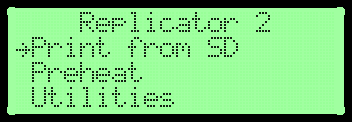
\includegraphics[]{main-01}
    \caption{Main Menu}
  \label{fig:main}
\end{figure}

You navigate the menus by using the keypad (Figure~\ref{fig:keypad})  on the front of the printer, which is generally located near the LCD screen:\index{Keys!Keypad}\index{Buttons|see {Keys}}\index{Menus!Navigating}

\begin{figure}[!htbp]
  \centering
\ifpdf
    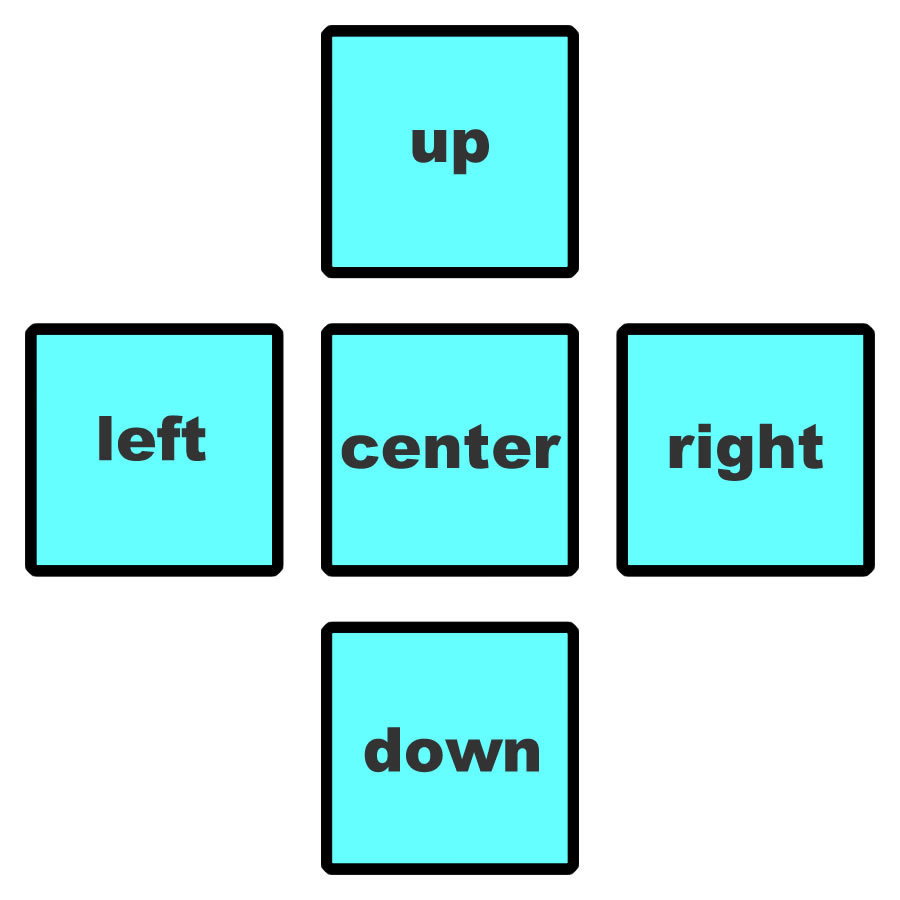
\includegraphics[]{keypad}
\else
    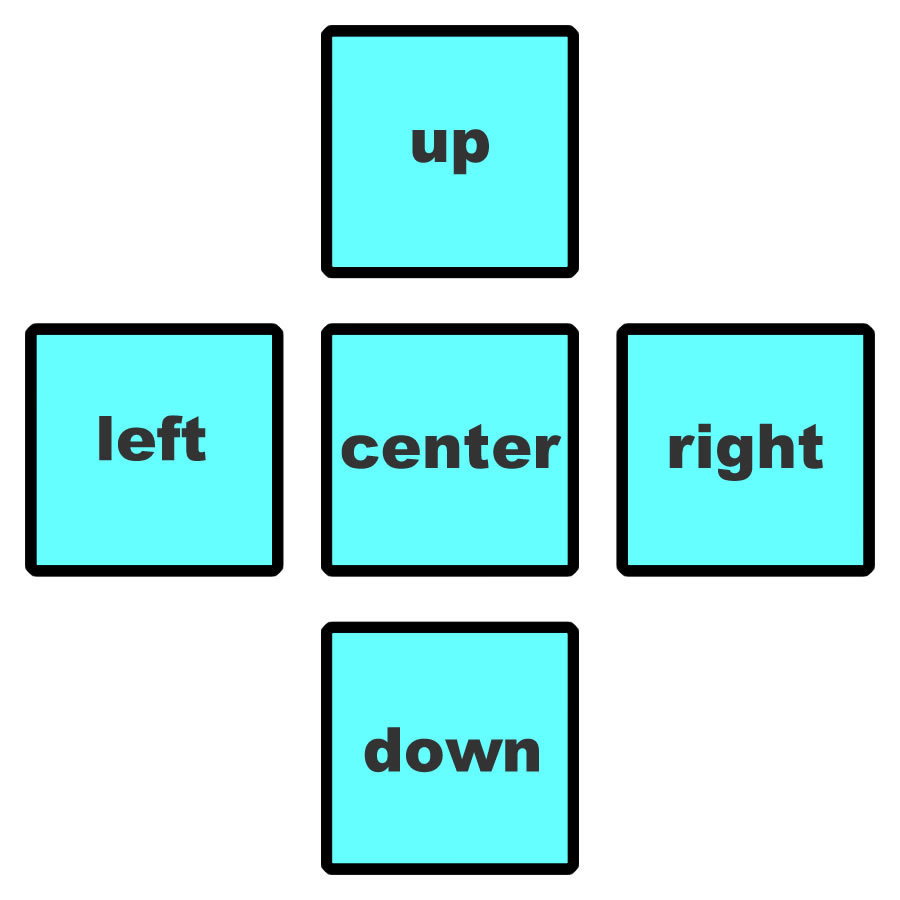
\includegraphics[width=3in]{keypad}
\fi
    \caption{Keypad}
  \label{fig:keypad}
\end{figure}

\begin{enumerate}
\item The up and down keys allow you to scroll through the list, which wraps around (so, if you scroll down from the bottom of the list you will return to the top of the list).\index{Keys!Up}\index{Keys!Down}
\item The center key (which, on some printers, has an ``M'' printed on it) allows you to select the item that has an arrow pointing to it.  In Figure~\ref{fig:main} this is the ``Print from SD'' item.  You can also dismiss any error message by pressing this key, which will then return you to the main menu.\index{Keys!Center}
\item The left key allows you to exit a menu and return to the previous menu.  Note that many menus have an ``Exit Menu'' option that will also return you to the previous menu.\index{Keys!Left}
\item Within the Jog Mode (Section~\ref{sec:jog}), Profiles: Change Name (Section~\ref{sec:profiles}), and Pause at ZPos (Section~\ref{sec:zpos}) menus where the right key is used, its function is described.  Otherwise, pressing the right key will reinitialize and repaint the LCD screen.\index{Keys!Right}
\end{enumerate}

\ifpdf
Table~\ref{tab:menu-tree} outlines the hierarchy of menus accessible through the front panel.
\fi

\ifpdf
\ifdefined\htmlflag
\else
\noindent
{\relsize{-1}
\begin{table}[!hb]
\begin{tabular}{lllll}
\hhline{~~|-|~~}
&& \cellcolor{LightBlue} \hyperref[sec:printmon]{Return to Monitor} \\
\hhline{~~|-|~~}
&& \cellcolor{LightBlue!50} \hyperref[sec:cancel]{Cancel Print} \\
\hhline{~~|-|~~}
&& \cellcolor{LightBlue} \hyperref[sec:pause]{Pause} \\
\hhline{~~|-|~~}
&& \cellcolor{LightBlue!50} \hyperref[sec:zpos]{Pause at ZPos} \\
\hhline{~~|-|~~}
&& \cellcolor{LightBlue} \hyperref[sec:speed]{Change Speed} \\
\hhline{~~|-|~~}
&& \cellcolor{LightBlue!50} \hyperref[sec:temp]{Change Temperature} \\
\hhline{~~|-|~|-|}
&& \cellcolor{LightBlue} \hyperref[sec:cooling]{Set Cooling Fan} && \cellcolor{LightCyan} \hyperref[sec:ditto]{Ditto Printing} \\
\hhline{~~|-|~|-|}
&& \cellcolor{LightBlue!50} \hyperref[sec:printstat]{Print Statistics} && \cellcolor{LightCyan} \hyperref[sec:override]{Override GcTemp} \\
\hhline{|-|-|-|~|-|}
\multicolumn{2}{l}{\cellcolor{LightBlue} \hyperref[sec:sdmenu]{Print from {\relsize{-0.5}SD}} \hfil $\Longrightarrow$ \hfil} & \cellcolor{LightBlue} \hyperref[sec:cold]{Cold Pause} && \cellcolor{LightCyan} \hyperref[sec:pauseheat]{Pause with Heat} \\
\hhline{|-|-|-|~|-|}
\cellcolor{LightCyan} \hyperref[sec:preheat]{Preheat} \phantom{om SD} &&&& \cellcolor{LightCyan} \hyperref[sec:sound]{Sound}  \\
\hhline{|-|-|-|~|-|}
\multicolumn{2}{l}{\cellcolor{LightBlue} \hyperref[sec:utilities]{Utilities} \hfil\phantom{mmm}\hfil $\Longrightarrow$} & \cellcolor{LightBlue} \hyperref[sec:monmode]{Monitor Mode} && \cellcolor{LightCyan} \hyperref[sec:acceleration-enable]{Acceleration} \\
\hhline{|-|-|-|~|-|}
&& \cellcolor{LightCyan} \hyperref[sec:filload]{Filament Loading} && \cellcolor{LightCyan} \hyperref[sec:extruder-count]{Extruder Count} \\
\hhline{~~|-|~|-|}
&& \cellcolor{LightBlue} \hyperref[sec:preheatset]{Preheat Settings} && \cellcolor{LightCyan} \hyperref[sec:extruder-hold]{Extruder Hold} \\
\hhline{~~|-|-|-|}
&& \multicolumn{2}{l}{\cellcolor{LightCyan} \hyperref[sec:general]{General Settings} \hfil\phantom{mmm} \hfil $\Longrightarrow$} & \cellcolor{LightCyan} \hyperref[sec:hbp-present]{HBP Installed} \\
\hhline{~~|-|-|-|}
&& \cellcolor{LightBlue} \hyperref[sec:levelbp]{Level Build Plate} && \cellcolor{LightCyan} \hyperref[sec:sd-crc]{Check SD Reads} \\
\hhline{~~|-|~|-|}
&& \cellcolor{LightCyan} \hyperref[sec:home-axes]{Home Axes} && \cellcolor{LightCyan} \hyperref[sec:pstop-enable]{P-Stop Control} \\
\hhline{~~|-|~~}
&& \cellcolor{LightBlue} \hyperref[sec:bot-stats]{Bot Statistics} \\
\hhline{~~|-|~~}
&& \cellcolor{LightCyan} \hyperref[sec:filodo]{Filament Odometer} \\
\hhline{~~|-|-|-|}
&& \multicolumn{2}{l}{\cellcolor{LightBlue} \hyperref[sec:profiles]{Profiles} \hfil\phantom{nmmmmmmm} \hfil $\Longrightarrow$} & \cellcolor{LightBlue} \hyperref[sec:profiles-r]{Restore} \\
\hhline{~~|-|-|-|}
&& \cellcolor{LightCyan} \hyperref[sec:homeoff]{Home Offsets} && \cellcolor{LightBlue} \hyperref[sec:profiles-dc]{Display Config} \\
\hhline{~~|-|~|-|}
&& \cellcolor{LightBlue} \hyperref[sec:tooloff]{Toolhed Offsets} && \cellcolor{LightBlue} \hyperref[sec:profiles-cn]{Change Name} \\
\hhline{~~|-|~|-|}
&& \cellcolor{LightCyan} \hyperref[sec:jog]{Jog Mode} && \cellcolor{LightBlue} \hyperref[sec:profiles-sp]{Save to Profile} \\
\hhline{~~|-|~|-|}
&& \cellcolor{LightBlue} \hyperref[sec:steppers-enable]{Enable/Disable Steppers} \\
\hhline{~~|-|~~}
&& \cellcolor{LightCyan} \hyperref[sec:alevel-variance]{Auto-level Variance} \\
\hhline{~~|-|~~}
&& \cellcolor{LightBlue} \hyperref[sec:alevel-maxhits]{Max Z Probe Hits} \\
\hhline{~~|-|~~}
&& \cellcolor{LightCyan} \hyperref[sec:calibnozz]{Calibrate Nozzles} \\
\hhline{~~|-|~~}
&& \cellcolor{LightBlue} \hyperref[sec:restore-settings]{Restore Settings} \\
\hhline{~~|-|~|-|}
&&  \multicolumn{2}{l}{\cellcolor{LightCyan} \hyperref[sec:eeprom]{EEPROM} \hfil\phantom{nmmmmmm} \hfil $\Longrightarrow$} & \cellcolor{LightCyan} \hyperref[sec:eeprom]{Eeprom -\textgreater\ SD} \\
\hhline{~~|-|~|-|}
&& \cellcolor{LightBlue} \hyperref[sec:versinf]{Version Information} && \cellcolor{LightCyan} \hyperref[sec:eeprom]{SD -\textgreater\ Eeprom} \\
\hhline{~~~~|-|}
&&&& \cellcolor{LightCyan} \hyperref[sec:eeprom]{Erase Eeprom} \\
\hhline{~~~~|-|}
\end{tabular}
\caption[Front panel menu hierarchy]{Front panel menu hierarchy}
\label{tab:menu-tree}
\end{table}
}
\fi
\fi


\NextFile{ui-print-from-sd-menu.html}

\section{Print from SD Menu}\label{sec:sdmenu}
\index{Menus!Print from SD}
\index{SD card}
\index{Flashcard|see {SD card}}
\index{Printing!Starting a print}

This menu allows you to print items you have already saved on an \gls{SD card} (also called a flashcard), which provides you the ability to print without connecting your printer to a computer.  When you open this menu, you should see a list of the items saved on your SD card.  An example menu is shown in Figure~\ref{fig:sdmenu}.  The last item on the menu is an ``Exit Menu'' shortcut that will return you to the main menu.

\begin{figure}[!htbp]
  \centering
    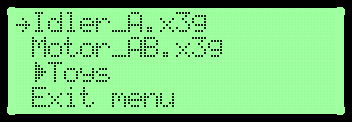
\includegraphics[]{printsd-01}
    \caption{SD Menu}
  \label{fig:sdmenu}
\end{figure}

\ifpdf
\pagebreak[4]
\fi

If instead, you see the error message ``SD card not present'' then you need to insert an SD card into your printer.\index{Errors!SD card not present}

If the error message ``Unable to read this SD card format.  Reformat as FAT-16 or FAT-32'' is displayed, then you need to remove your SD card and reformat it.\index{Errors!Unable to read this SD card format...}  The SD card \emph{must} be formatted as \gls{FAT-16}.\index{SD card!Format}  Unlike standard MakerBot firmware (which only supports FAT-16 on SDSC cards of 2 GB or less), any capacity of SD card may be used, including SDSC (standard capacity), SDHC (high capacity), and SDXC (extended capacity) cards.  Note that many new SD cards now come formatted using the proprietary, licensed ``eFAT'' format.  Sailfish does not support this format as implementation requires licensing from Microsoft.  If you have difficulty with a new SD card, you may wish to check its format on your computer, reformatting it as ``FAT'' if necessary.

To print an item, scroll to it and then press the center key; this will start the printing of the model, displaying the print monitor screen. %name  
\index{SD card!Files not appearing|(}If you are unable to see or print an item saved on your card, you should reformat the files on the SD card.  Items should be saved as \glspl{X3G} or \glspl{S3G} files (not case sensitive) with filenames 31 or fewer characters including extension. It is best to use simple filenames that do not include spaces, accents, or other special characters.\index{SD card!File names}\footnote{Note that \texttt{.s3g} is an older type of file, so you may wish to consider regenerating any \texttt{.s3g} files on your computer as \texttt{.x3g} files.}

If you are still unable to find an item, it may be in a folder.  In Figure~\ref{fig:sdmenu} the item ``Toys'' is a folder, as indicated by the solid triangle.\index{SD card!Folders}
Folders can be opened by pressing the center key, which will take you to a submenu (See Figure~\ref{fig:submenu}).  For this reason, folders are useful organizational tools if you have many items on your SD card.\index{SD card!Files not appearing|)}

\begin{figure}[!htbp]
  \centering
    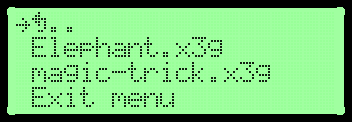
\includegraphics[]{printsd-02}
    \caption{SD ``Toys'' Submenu}
  \label{fig:submenu}
\end{figure}

Note that if you either press the left key or select the return symbol from within a folder, you return to the previous folder or screen, while the ``Exit Menu'' shortcut returns you to the main menu.  For your convenience, if you have returned to the main menu from the ``Exit Menu'' shortcut, when you return to the ``Print from SD'' menu, you return to whichever folder you had been in.  Note that if you remove the SD card and reinsert it this folder state is lost.  Likewise, the folder state is lost when you power off your printer.

\NextFile{ui-print-monitor-menu.html}

\section{Starting a Print: the Print Monitor \& Menu}\label{sec:printmon}
\index{Printing!Starting a print}
\index{Printing!Monitor screen}
\index{Screens!Print monitor}

Once you start a print from the ``Print from SD'' menu (Section~\ref{sec:sdmenu}), the LCD screen should display the print monitor.  By pressing the center key you can exit the print monitor to access the print menu.

If you have not preheated your printer, the screen will display a heating progress bar on the first line, as seen in Figure~\ref{fig:printpreheat}.

\begin{figure}[!htbp]
  \centering
    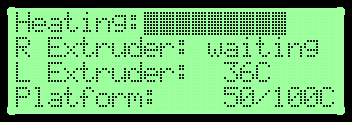
\includegraphics[]{printing-02}
    \caption{Print Monitor --- Preheating}
  \label{fig:printpreheat}
\end{figure}
  
The screen should also display the current temperatures and target temperatures (in Celsius) of all your heating elements in the form current temperature/target temperature --- if, however, the element is not going to be heated, then it will only display its current temperature.  Note that for some printers the extruders do not start heating until the platform has heated (such as genuine MakerBots with smaller power supplies).  In this case the screen will display ``waiting'' rather than the temperatures.\index{Waiting temperature}  In addition, the number of heating elements displayed will depend on the number your printer has.  Figure~\ref{fig:printpreheat} shows a dual extruder set-up.

Once your printer has finished heating, the heating progress bar is replaced by a line displaying the name of the print (which will be the name on the SD card unless print commands in the file change the displayed name) and the percentage completed of the print (Figure~\ref{fig:print}).  Since the percentage is generated by the \gls{slicer}, it will remain displayed as 0\% if the file does not contain print commands to update it.  If a future Pause at Z-Position is scheduled (Section \ref{sec:zpos}), then an asterisk will appear before the percentage.\index{Percentages, build}

\begin{figure}[!htbp]
  \centering
    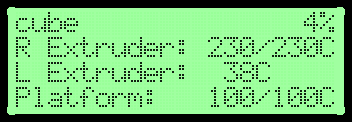
\includegraphics[]{printing-03}
    \caption{Print Monitor --- Printing}
  \label{fig:print}
\end{figure}

On \emph{some} printers with only two heating elements the firmware uses the extra available line to display a running ticker of statistics:\index{Printing!Ticker display}
\begin{enumerate}
\item The elapsed build time.\index{Printing!Elapsed time}
\item The estimated build time remaining.  This will only be generated if the print commands include the percentage complete updates and is, therefore, only as accurate as the percentage markers.\index{Printing!Estimated time left}
\item The current filament usage.\index{Printing!Filament usage}\index{Filament!Usage}
\item The current Z position.\index{Printing!Current build height}
\end{enumerate}
If this ticker is not displayed, the information can be accessed in the ``Print Statistics'' item under the print menu, Section~\ref{sec:printstat}.

By pressing the center key to dismiss the print monitor, you can access the print menu, seen in Figure \ref{fig:printeth-menueth}.

\begin{figure}[!htbp]
  \centering
    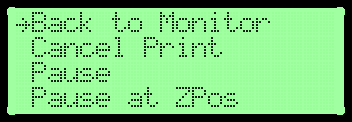
\includegraphics[]{printing-04}
    \caption{The first screen of the print menu}
  \label{fig:printeth-menueth}
\end{figure}

The print menu allows you to control aspects of the printing process as well as monitor the printing progress:\index{Menus!Print menu}
\begin{enumerate}
\item Back to Monitor: returns you to the print monitor.
\item Cancel Print: as the name suggests, this allows the termination of the print.  A confirmation screen will be generated to prevent accidental termination.
\item Pause: by allowing you to suspend a print and generating the pause menu, the pause option lets you change aspects of the print.  If the printer is left paused for over 30 minutes the heaters will turn off even if ``Pause with Heat'' is enabled (Section~\ref{sec:pauseheat}).
\item Pause at ZPos: lets you program the print to stop at a certain height.  Once the printer pauses, the pause menu will be generated.  Again, if the printer is left paused for over 30 minutes the heaters will turn off even if ``Pause with Heat'' is enabled.\footnote{Commands to pause at specified heights may be placed directly in a print file; see Section~\ref{sec:special-gcode}.}
\item Change Speed.
\item Change Temperature.
\item Set Cooling Fan ON/OFF.
\item Print Statistics: displays the elapsed build time, the estimated build time remaining for prints with percentage complete updates, the current filament usage, and the current Z position. 
\item Cold Pause: pauses, cools off all heating elements, turns off LED lighting, and generates the pause menu.
\end{enumerate}

\NextFile{ui-print-monitor-menu-cancel-print.html}

\subsection{Cancel Print}\label{sec:cancel}
\index{Printing!Canceling}

To cancel a print while printing, choose the ``Cancel Print'' item under the print menu.  Do not just turn off the printer, as that can damage the printer.  Choosing this item will generate the confirmation screen pictured below in Figure~\ref{fig:cancel}.

\begin{figure}[!htbp]
  \centering
    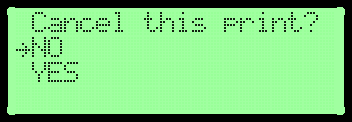
\includegraphics[]{printing-05}
    \caption{Cancel Print Confirmation}
  \label{fig:cancel}
\end{figure}

Once you have canceled the print, the printer will cease printing and move your print away from the extruders by lowering the build platform.  All the heaters will be switched off.

\NextFile{ui-print-monitor-menu-pause.html}

\subsection{Pause}\label{sec:pause}
\index{Printing!Pausing}
\index{Pausing}

Pausing your printer generates the pause menu, which allows you to change aspects of the print that cannot otherwise be changed in the middle of printing.  The pause is not immediate, as the printer will continue printing until it clears out its buffer of queued work.  The LCD screen will acknowledge this and generate the screen as seen in Figure~\ref{fig:clear}.

\begin{figure}[!htbp]
  \centering
    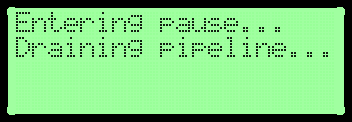
\includegraphics[]{pause-drain}
    \caption{Clearing Queue}
  \label{fig:clear}
\end{figure}

When your printer starts to pause, you should see the screen shown in Figure~\ref{fig:startpause}.

\begin{figure}[!htbp]
  \centering
    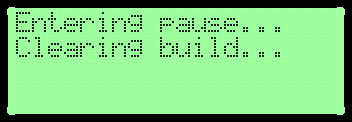
\includegraphics[]{pause-clear}
    \caption{Pause}
  \label{fig:startpause}
\end{figure}

Once your printer is paused, the pause menu appears:\index{Menus!Pause}

\begin{enumerate}
\item Jog Mode: shift the platform or extruder along the X, Y, and Z axes.  Be careful not to hit the endstops, as that will cause a loss of registration and the print will not resume in the proper place.  The jog mode is identical to ``Jog Mode'' in the ``Utilities'' menu; for operation details see Section~\ref{sec:jog}.
\item Filament Loading: allows you to load and unload filament.  As this is identical to ``Filament Loading'' in the ``Utilities'' menu, see Section~\ref{sec:filload}.
\item Heaters Off: turns off all heaters.  Again, note that if the printer is paused for over 30 minutes the heating units should turn off automatically even if ``Pause with Heat'' is enabled, Section~\ref{sec:pauseheat}.
\end{enumerate}

To resume printing select the ``Unpause'' item on the pause menu.  You should see the screen pictured in Figure~\ref{fig:endpause}.\index{Printing!Resuming}  Note that if the print has been paused for an extended period, it is best to run the filament load for 10--30 seconds to purge the extruder of cooked plastic.  If the extruder is sitting over your print, use the jog controls to move it over a clear spot.  

\begin{figure}[!htbp]
  \centering
    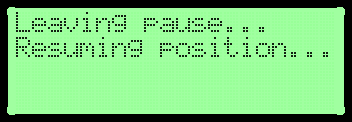
\includegraphics[]{unpause-resume}
    \caption{Unpause}
  \label{fig:endpause}
\end{figure}

\NextFile{ui-print-monitor-menu-pause-at-zpos.html}

\subsection{Pause at ZPos}\label{sec:zpos}
\index{Pause at ZPos}
\index{Printing!Pausing at a set height}
\index{Printing!Pause @ ZPos}
\index{Pausing!Specified build height}

This programs the printer to pause when it first attains or exceeds a specified height.  Choosing this item will generate the screen depicted in Figure~\ref{fig:Zpause}.

\begin{figure}[!htbp]
  \centering
    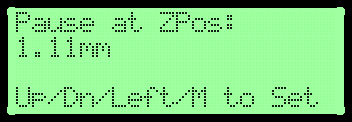
\includegraphics[]{printing-10}
    \caption{Pause at ZPos}
  \label{fig:Zpause}
\end{figure}

To change the Z position use the up and down keys, and to set the Z position press the center key.  Pressing the right key once changes the Z position in larger increments, a second causes larger increment still, but a third time will set the value by which it increments back to the original; it is actually doing this in units of steps, but still displays units of millimeters.  Pressing the left key cancels any changes to the Pause at Z-Position value.

Note that the printer continues printing while you set the Z position.

Since you can include multiple pauses at specified Z positions within the printing file, the printer honors the last pause it has received.  Therefore, if it encounters a pause within the printing file after you manually set one, it will replace the Pause at Z-Position that you have set with the one in the print file.  Likewise, if you have included pauses within the print file, they will be replaced by any subsequent pauses you enter manually.

If you set a Pause at Z-Position and later wish to cancel any such pause you can either allow it to pause and then manually resume right after, or set the Z position for the pause to a value not attained by the print.  Note that each print starts without a Pause at Z-Position set --- the changes are not retained between prints.

When using Pause at ZPos it is important to note that the \gls{slicer} probably started your model a few hundredths of a millimeter above zero so you need to account for this difference when setting a pause height.

Once the print has attained the specified height, the pause menu (Section~\ref{sec:pause}) will be generated.

\NextFile{ui-print-monitor-menu-change-speed.html}

\subsection{Change Speed}\label{sec:speed}
\index{Printing!Changing speed}

This item allows you to change the printing speed by a multiplicative factor (see Figure~\ref{fig:speed}).  \emph{As you enter the speed}, it starts percolating through the queue of already buffered work.

\begin{figure}[!htbp]
  \centering
    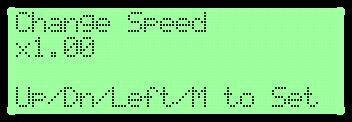
\includegraphics[]{printing-12}
    \caption{Change Speed}
  \label{fig:speed}
\end{figure}

To increase the speed use the up key, and to decrease it use the down key.  The center key will set the speed and return you to the print menu while the left key will cancel any changes and return you to the print menu.  Note that pressing the left key will \emph{not} necessarily return the speed to 1.00, rather, it reinstates the scaling factor which was in effect when the screen was entered.

\NextFile{ui-print-monitor-menu-change-temperature.html}

\subsection{Change Temperature}\label{sec:temp}
\index{Printing!Changing temperature}

This allows you to change the temperature of the currently active extruder while printing.  You cannot use this menu (see Figure~\ref{fig:printtemp}) to change the heated platform's temperature or the temperature of an inactive extruder.

\begin{figure}[!htbp]
  \centering
    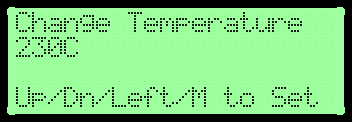
\includegraphics[]{printing-13}
    \caption{Change Temperature}
  \label{fig:printtemp}
\end{figure}

To increase the temperature use the up key; to decrease it use the down key.  You cannot set the temperature above 280\textdegree\,C and, naturally, you also do not wish to set it too low or else the filament will not melt.

Unlike the change speed item, the temperature changes do not take effect until the center key is pressed.  Pressing this key sets the temperature and returns you to the print menu.  Note that if you change the temperature by more than 10\textdegree\,C at a time the algorithm used by the temperature control will reset, which can cause temperature instability for upwards of a minute.  Pressing the left key cancels any change in temperature, resetting the temperature to what it had been, and returns you to the print menu.

\NextFile{ui-print-monitor-menu-set-cooling-fan.html}

\subsection{Set Cooling Fan}\label{sec:cooling}
\index{Cooling fan}
\index{Printing!Cooling fan}

This allows you to change the state of the \gls{print cooling fan} on printers that have such a fan.  Note that this has nothing to do with the \glspl{heatsink cooling fan}.  If the cooling fan is currently off, then the option will read ``Set Cooling Fan ON'' as depicted in Figure~\ref{fig:coolingfan} below.  Likewise, if the cooling fan is on, then the option will read ``Set Cooling Fan OFF''.

\begin{figure}[!htbp]
  \centering
    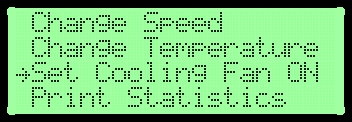
\includegraphics[]{printing-15}
    \caption{Set Cooling Fan}
  \label{fig:coolingfan}
\end{figure}

Note that some \glspl{slicer} generate many commands to turn the fan on and off throughout the course of the print.  When you turn the fan on or off with this item, any subsequent print commands to change the fan's state \emph{will} be honored --- this option does not override all further print commands regarding the fan.

\NextFile{ui-print-monitor-menu-print-statistics.html}

\subsection{Print Statistics}\label{sec:printstat}
\index{Printing!Statistics}

This item (Figure~\ref{fig:printstatistics}) allows you to see the progress of the print as reflected in four items:
\begin{enumerate}
\item Print Time: the elapsed build time.\index{Printing!Elapsed time}
\item Time Left: the estimated build time remaining.  This will only be generated if the print commands include percentage complete updates and is, therefore, only as accurate as the percentage markers.\index{Printing!Estimated time left}
\item Filament: the length of filament used so far in meters.\index{Printing!Filament usage}\index{Filament!Usage}
\item ZPosition: the current Z position in mm.\index{Printing!Current build height}
\end{enumerate}

\begin{figure}[!htbp]
  \centering
    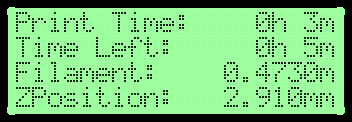
\includegraphics[]{printing-14}
    \caption{Print Statistics}
  \label{fig:printstatistics}
\end{figure}

If your firmware has auto-leveling, then the last line will alternate between auto-leveling status and Z position, displaying one for a few seconds and then the other.

\NextFile{ui-print-monitor-menu-cold-pause.html}

\subsection{Cold Pause}\label{sec:cold}
\index{Printing!Cold pause}
\index{Pausing!Cold}

This option allows you to pause the print and automatically turn off the heaters and LEDs.  This will also generate the pause menu, Section~\ref{sec:pause}.

\NextFile{ui-completing-a-print.html}

\section{Completing a Print} \label{sec:print-done}

Once the print is completed, the LCD generates a screen similar to the one shown in Figure~\ref{fig:printcomplete}.

\begin{figure}[!htbp]
  \centering
    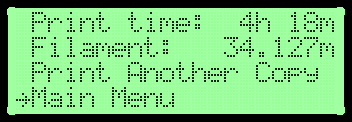
\includegraphics[]{finish-01}
    \caption{Print From SD Card Complete}
  \label{fig:printcomplete}
\end{figure}

This screen shows how long the print took (in hours and minutes) and how much filament was used (in meters).  You are also given the options of either reprinting the item or returning to the main menu.  If you choose to print another copy, you \emph{must} first clear the build plate before selecting ``Print Another Copy'', as the reprint will then begin \emph{immediately}.  Note that pressing the left key will also return you to the main menu.

If you instead printed over USB, you should see a screen similar to the one in Figure~\ref{fig:usbprint} below.  The only difference is that the option of printing another copy is not available.

\begin{figure}[!htbp]
  \centering
    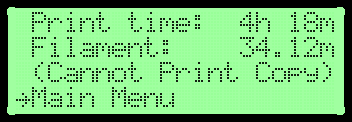
\includegraphics[]{finish-02}
    \caption{Print From USB Complete}
  \label{fig:usbprint}
\end{figure}

\NextFile{ui-preheat-menu.html}

\section{Preheat Menu}\label{sec:preheat}
\index{Menus!Preheat}
\index{Preheat}
\index{Printing!Preheat}

This menu can be used to begin heating your printer without starting printing.  Doing this directly before starting a print will reduce the time it takes for the print.  The screen generated varies depending on the number of extruders that your printer has.  A dual extruder set-up should display a screen similar to the one depicted in Figure~\ref{fig:preheat}.  Note that the ``Platform'' line will only appear if your printer is equipped with a heated build platform.\index{Heated build platform!Preheating}

\begin{figure}[!htbp]
  \centering
    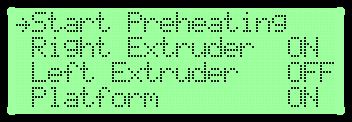
\includegraphics[]{preheat-01}
    \caption{Preheat Menu}
  \label{fig:preheat}
\end{figure}

To turn a heater on or off scroll to its line and then press the center key to toggle it between ``ON'' and ``OFF''.  Then, once you have set which heaters you wish to have on, select the option ``Start Preheating''.\index{Preheat!On}  The enabled heaters will begin heating and the ``Monitor Mode'' screen will be generated.  The ``Monitor Mode'' screen can also be found under the ``Utilities'' menu, and is discussed Section~\ref{sec:monmode}.  This screen should be similar to the one depicted in Figure~\ref{fig:heat}.

\begin{figure}[!htbp]
  \centering
    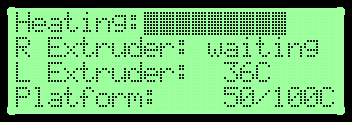
\includegraphics[]{printing-02}
    \caption{Preheating}
  \label{fig:heat}
\end{figure}

The top bar measures the preheating progress.  The current temperatures (in Celsius) of all the heating elements will be displayed next to the target temperatures in the form current temperature/target temperature.  The target temperature may be changed in the ``Preheat Settings'' item in the ``Utilities'' menu, Section~\ref{sec:preheatset}.  The screen will display ``waiting'' if an element has not begun heating yet.  Some printers with smaller power supplies, such as genuine MakerBots, do not heat the extruders until the heated build platform has reached temperature.\footnote{Also, MakerWare and Simplify3D will not even send commands to heat the extruders until the heated build platform has finished heating.}

You may dismiss the monitor and return to the main menu by pressing either the center or left key.

If the heaters are already running, then the first line of the Preheat screen will read ``Turn Heaters OFF,'' as shown in Figure~\ref{fig:endheat}.\index{Preheat!Off}

\begin{figure}[!htbp]
  \centering
    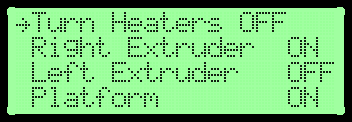
\includegraphics[]{preheat-03}
    \caption{End Preheating}
  \label{fig:endheat}
\end{figure}

By selecting this you turn off \emph{all} the heaters and return to the ``Monitor Mode'' screen, Figure~\ref{fig:heat}.  The first line there will now display the printer's name and the following lines will show only the \emph{current} temperatures.  %image

\NextFile{ui-utilities-menu.html}

\section{Utilities Menu}\label{sec:utilities}
\index{Menus!Utilities}
\index{Utilities}

The utilities menu is accessible from the main menu, Section~\ref{sec:Main}.  Figure \ref{fig:utilitiesfirstscreen} shows the first screen of the utilities menu.

\begin{figure}[!htbp]
  \centering
    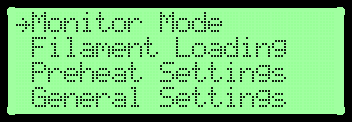
\includegraphics[]{utilities-01}
    \caption{Utilities Menu}
  \label{fig:utilitiesfirstscreen}
\end{figure}

\NextFile{ui-utilities-menu-monitor-mode.html}

\subsection{Monitor Mode} \label{sec:monmode}
\index{Screens!Monitor mode}
\index{Utilities!Monitor mode}

This screen shows you the current temperatures of all your heating elements.  If any of them are enabled, the screen will also show the target temperatures and the heating progress bar as seen in Figure~\ref{fig:heatmonmode}.

\begin{figure}[!htbp]
  \centering
    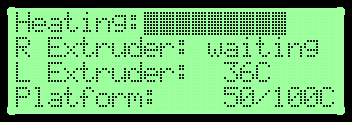
\includegraphics[]{printing-02}
    \caption{Monitor Mode}
  \label{fig:heatmonmode}
\end{figure}

Note that the build platform's current temperature may be as much as 10\textdegree\,C off from that of the extruders when unheated, as the build platform uses a different temperature sensor than the extruders --- one that is more accurate at operating temperatures and less so at room temperature.

\NextFile{ui-utilities-menu-filament-loading.html}

\subsection{Filament Loading} \label{sec:filload}
\index{Utilities!Filament loading}
\index{Filament!Loading}
\index{Filament!Unloading}

This option allows you to load, unload, and change filament in any extruder.  Selecting this option will allow you to choose (if relevant to your printer) which extruder to load or unload.  You will see a screen similar to the one shown in Figure~\ref{fig:filload}, dependent on the number of extruders with which your printer is equipped.

\begin{figure}[!htbp]
  \centering
    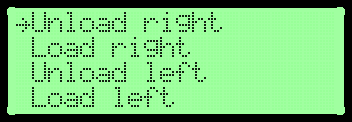
\includegraphics[]{load-01}
    \caption{Filament Loading}
  \label{fig:filload}
\end{figure}

Once you have chosen which extruder for which to change the filament, the printer will begin heating that extruder if necessary, generating a heating progress bar as well as the current and target temperatures, as seen in Figure~\ref{fig:filheat}.  As indicated, press the left key to cancel the operation.  Note that the extruder will be heated up to its preheat temperature, which may be changed in the ``Preheat Settings'' under the ``Utilities'' menu, Section~\ref{sec:preheatset}.

\begin{figure}[!htbp]
  \centering
    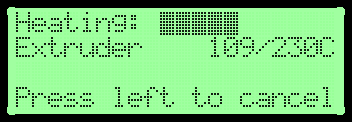
\includegraphics[]{load-03}
    \caption{Extruder Heating}
  \label{fig:filheat}
\end{figure}

Once the extruder is at the proper temperature, a screen similar to the one shown in Figure~\ref{fig:filpro} will be generated.

\begin{figure}[!htbp]
  \centering
    
\includegraphics[]{load-04}
    \caption{Loading or Unloading}
  \label{fig:filpro}
\end{figure}

At this point you may manually load, unload, or change the filament.  The printer will automatically turn on the proper extruder's stepper motor, allowing the filament to be fed in or backed out.  Note that while pressing the center key will return you to the ``Filament Loading'' menu, pressing the left key will generate a screen asking if you wish to cancel.  To confirm the cancellation, select ``Yes'' and press the center key.

\NextFile{ui-utilities-menu-preheat-settings.html}

\subsection{Preheat Settings} \label{sec:preheatset}
\index{Preheat!Temperatures}
\index{Utilities!Preheat settings}
\index{Menus!Preheat settings}

This option allows you to set the preheat temperatures for each of the heating elements.  Temperatures are all in degrees Celsius.  This option displays the screen shown in Figure~\ref{fig:preset}.  As always, the number of extruders listed will depend on the number your printer has.

 \begin{figure}[!htbp]
  \centering
    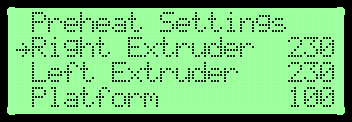
\includegraphics[]{preheat-settings-01}
    \caption{Preheat Setting}
  \label{fig:preset}
\end{figure}

To change the temperature for a heated element, select it and press the center key, then use the up key to increase the temperature and the down key to decrease it.  To save the changes to a temperature, press the center key.  The left key is used to exit the menu and return to ``Utilities''.  The maximum temperature that the firmware will allow you to set is 280\textdegree\,C for the extruders, and 130\textdegree\,C for the build platform.\index{Temperature!Maximums}

\NextFile{ui-utilities-menu-general-settings.html}

\subsection{General Settings} \label{sec:general}
\index{Utilities!General settings}
\index{Menus!General settings}

This menu allows you to change many simple settings.  The screen will show you up to four options at once.  To choose an option press the center key.  You may then use the up and down keys to toggle between two choices for that setting and press the center key to save the change.  The left key will exit the menu and return you to ``Utilities''.

\NextFile{ui-utilities-menu-general-settings-ditto-printing.html}

\subsubsection{Ditto Printing} \label{sec:ditto}
\index{Ditto printing}
\index{Printing!Ditto}
\index{Parameters!Ditto}

If you have more than one extruder, than this option allows you to reproduce the print for a second extruder, enabling you to print two of the same thing at once.  It does not matter for which extruder the print was sliced, it will be reproduced on both.  You do have to make sure that on no given layer will the two nozzles interfere with each other.  If you only have one extruder, this option will display the text ``N/A'' as it is unavailable.  By default, this feature is disabled. %clever ditto printing examples?

 \begin{figure}[!htbp]
  \centering
    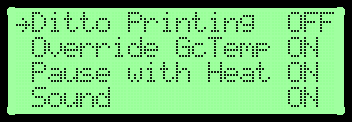
\includegraphics[]{general-01}
    \caption{General Settings --- First Screen}
  \label{fig:genfirst}
\end{figure}

\NextFile{ui-utilities-menu-general-settings-override-gctemp.html}

\subsubsection{Override GcTemp} \label{sec:override}
\index{Overriding temperatures}
\index{Temperature!Overriding}
\index{Printing!Overriding temperatures}
\index{Parameters!Override gcode temperature}

When enabled, this option allows you to override the non-zero temperatures in a print file.  These temperatures will be replaced by the preheat temperature for the given heater.  This is useful for experimentation or for switching plastics without reslicing.  By default, this feature is disabled.

\NextFile{ui-utilities-menu-general-settings-pause-with-heat.html}

\subsubsection{Pause with Heat} \label{sec:pauseheat}
\index{Pausing!Leaving heaters on}
\index{Parameters!Pause with heat}

If this option is enabled, it allows the heaters to remain on when a print is paused.  However, even if ``Pause with Heat'' is enabled the heaters will turn off after the print is paused for over 30 minutes due to safety reasons.  By default, this feature is disabled.

\NextFile{ui-utilities-menu-general-settings-sound.html}

\subsubsection{Sound} \label{sec:sound}
\index{Parameters!Sound}
\index{Buzzer}
\index{Sound}

If you are annoyed by the buzzer, use this option to turn it off.  The buzzer normally sounds when the printer turns on to tell you the firmware has started, the announcement of some warning messages is accompanied by the buzzer, and print files can include tunes played on the buzzer.  By default, this feature is enabled.

\NextFile{ui-utilities-menu-general-settings-acceleration.html}

\subsubsection{Acceleration} \label{sec:acceleration-enable}
\index{Parameters!Acceleration}
\index{Acceleration!Disabling}

This enables the printer's use of acceleration when effecting move commands.  When acceleration is disabled, the printer will attempt to instantaneously jump to the requested speeds, causing more jerks and vibrations.  If you wish to print with acceleration disabled, print at speeds closer to 30--40~mm/s, as printing at high speeds with acceleration disabled can both damage the printer as well as ruin your print.  By default, this feature is enabled.

 \begin{figure}[!htbp]
  \centering
    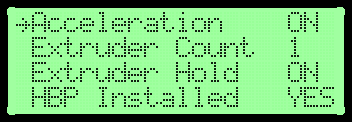
\includegraphics[]{general-02}
    \caption{General Settings --- Second Screen}
  \label{fig:gen2}
\end{figure}

\NextFile{ui-utilities-menu-general-settings-extruder-count.html}

\subsubsection{Extruder Count} \label{sec:extruder-count}
\index{Parameters!Extruder count}
\index{Tool count}
\index{Extruder count}

This tells the firmware the number of extruders with which your printer is equipped.  More than two extruders is not supported by standard Sailfish distributions.  The default extruder count depends on your type of printer.  The default is one for a Replicator 2, and two for all other printers.

After changing the extruder count, the printer should be power cycled for the change to take effect.

\NextFile{ui-utilities-menu-general-settings-extruder-hold.html}

\subsubsection{Extruder Hold} \label{sec:extruder-hold}
\index{Parameters!Extruder hold}

This is primarily meant for extruders that use 3 millimeter filament.  This ensures that, throughout the entire print, the extruder's stepper motor is kept engaged and does not allow the filament to creep out.  This is mostly a problem with extruders that accept 3 millimeter filament, as larger filament generates more back pressure.  Therefore, this option is intended to counteract the tendency of filament to back out of the extruder when the stepper motor is temporarily disabled, a command some \glspl{slicer} will add to the print command file (for instance, ReplicatorG).  For Cupcake printers the default is on; for all other printers, the default is off.

\NextFile{ui-utilities-menu-general-settings-hbp-installed.html}

\subsubsection{HBP Installed} \label{sec:hbp-present}
\index{Parameters!HBP installed}
\index{Heated build platform!Enabling}

This tells the firmware if your printer is equipped with a heated build platform.  The default is no for a Replicator 2, and yes for all other printers.

After changing the \gls{HBP} setting, the printer should be power cycled in order for the change to take effect.

\NextFile{ui-utilities-menu-general-settings-check-sd-reads.html}

\subsubsection{Check SD Reads} \label{sec:sd-crc}
\index{SD card!Error checking}
\index{SD card!CRC}
\index{Parameters!Check SD reads}

This allows you to check for errors when reading or writing to the SD card.  Typically, with this feature disabled, errors in reading or writing to the SD card may make the printer do something unexpected.  With this feature enabled, if an error is detected, the operation will be reattempted up to five times, at which point the print will be canceled.  Note that, enabling this feature this can affect performance when printing fine detail at high speeds.  By default, this feature is disabled.
 
 \begin{figure}[!htbp]
  \centering
    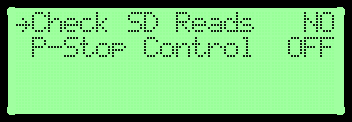
\includegraphics[]{general-03}
    \caption{General Settings --- Third Screen}
  \label{fig:gen3}
\end{figure}

\NextFile{ui-utilities-menu-general-settings-pstop-control.html}

\subsubsection{P-Stop Control} \label{sec:pstop-enable}
\index{Parameters!P-Stop}
\index{Pausing!P-Stop}
\index{Filament jam detector}
\index{P-Stop}

If you have equipped your printer with extra hardware (such as a filament jam detector) to trigger a build pause, then you will want to enable this feature.  When enabled, this allows extra hardware to tell the printer to pause a print, allowing you to fix any error condition and resume the print.  Do not enable this unless you have installed such hardware, as the printer will not function when it cannot detect any additional hardware.  Likewise, the extra hardware will be ignored if this is not enabled.  By default, this feature is disabled.

\NextFile{ui-utilities-menu-general-settings-serial-io.html}

\subsubsection{Serial I/O} \label{sec:alternate-uart}
\index{Parameters!Serial I/O}

Printers with ATmega~2560 microprocessors include an experimental option which allows all serial communications to be passed through the printer's alternate serial port, UART1, instead of the USB port.  When this option is set to the value ``UART1'' the USB port becomes non-functional: the printer will only communicate through the alternate serial port.

Presently, this option is being used by advanced users experimenting with Bluetooth, network, and other alternate forms of printer communications and control.  

\NextFile{ui-utilities-menu-level-build-plate.html}

\subsection{Level Build Plate} \label{sec:levelbp}
\index{Utilities!Level build plate}
\index{Leveling}

Choosing this option will home the axes, first X and Y, and then Z.  Once homed, the extruder will be moved to the center of the build plate, as defined in the ``Home Offsets'' section under the ``Utilities'' menu, Section~\ref{sec:homeoff}.  The X and Y stepper motors are then disabled, while the Z stepper motor is left enabled.

Now you can freely move the extruder to any position above the build plate in order to check if the build plate is level.  Sailfish does not require you to move the extruder to designated checkpoints, allowing you to go to the points you want to, in the order you want to, as many times as you want to.  

A screen will be generated explaining this procedure which may be dismissed by pressing the center key.  The fourth screen will tell you to press the center key to return to the ``Utilities'' menu and disengage the Z stepper motor when you are finished leveling the build plate.

\NextFile{ui-utilities-menu-home-axes.html}

\subsection{Home Axes} \label{sec:home-axes}
\index{Utilities!Home axes}
\index{Homing}

This is simply a convenience utility to home the axes for you.  This may be useful when diagnosing mechanical problems.

\NextFile{ui-utilities-menu-bot-statistics.html}

\subsection{Bot Statistics} \label{sec:bot-stats}
\index{Utilities!Bot statistics}
\index{Screens!Bot statistics}

This option displays usage information for your printer (Figure~\ref{fig:botstat}).

 \begin{figure}[!htbp]
  \centering
    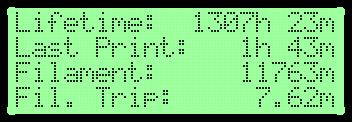
\includegraphics[]{botstats-01}
    \caption{Bot Statistics}
  \label{fig:botstat}
\end{figure}

\begin{enumerate}
\item The lifetime printing time in hours and minutes.\index{Printing!Lifetime usage}
\item The time spent on the last print in hours and minutes.\index{Printing!Last print time}
\item The lifetime filament length used in meters.\index{Filament!Usage}
\item The length of filament used since the filament trip odometer was last reset in meters or millimeters.  This can be reset in the ``Filament Odometer'' option under ``Utilities'', Section~\ref{sec:filodo}.\index{Printing!Filament last used}
\end{enumerate}

This menu may be exited by pressing either the center or left keys.

\NextFile{ui-utilities-menu-filament-odometer.html}

\subsection{Filament Odometer} \label{sec:filodo}
\index{Utilities!Filament odometer}
\index{Filament!Usage}
\index{Filament!Odometer}

This option shows a screen similar to the one depicted in Figure~\ref{fig:odo}.

 \begin{figure}[!htbp]
  \centering
    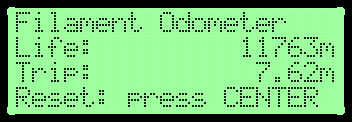
\includegraphics[]{odometer-01}
    \caption{Filament Odometer}
  \label{fig:odo}
\end{figure}

This displays the lifetime filament usage in meters or millimeters.  This also displays the amount of filament used since the filament trip odometer was last reset.  The odometer can be reset by pressing the center key.  To exit the menu, press the left key.

\NextFile{ui-utilities-menu-profiles.html}

\subsection{Profiles} \label{sec:profiles}
\index{Utilities!Profiles}
\index{Profiles}

This item lets you save up to four different sets of preheat and home offsets settings, and quickly recall them to enable ease of printing with different plastics, build surfaces, prints, slicers, etc.

The default names assigned to the profiles are ``ABS'', ``PLA'', ``Profile3'', and ``Profile4''.  You can change these names by selecting them, pressing the center key, and choosing the ``Change Name'' item of the profile
\ifpdf
menu.
\else
menu, Section~\ref{sec:profile-menu}.
\fi

\NextFile{ui-utilities-menu-profiles-profile-menu.html}

\subsubsection{Profile Menu} \label{sec:profile-menu}
\index{Menus!Profile}

Once you select one of the profiles, the profile menu will be generated.  It contains four items:

\begin{enumerate}
\item Restore:\label{sec:profiles-r} selecting this restores the saved home offsets and preheat temperatures, making them your current settings.  These settings will survive power cycles.  Selecting this will also return you to the ``Utilities'' menu, Section~\ref{sec:utilities}.
\item Display Config:\label{sec:profiles-dc} choosing this generates screens similar to the ones depicted in Figures~\ref{fig:cd1} and \ref{fig:cd2}.\index{Profiles!Displaying}

\begin{figure}[!htbp]
 \centering
    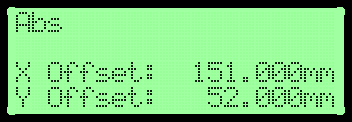
\includegraphics[]{profile-display-01}
    \caption{Configuration Display --- Screen 1}
  \label{fig:cd1}
\end{figure}

\begin{figure}[!htbp]
  \centering
    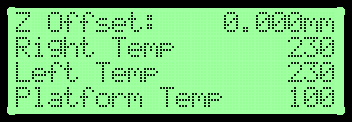
\includegraphics[]{profile-display-02}
    \caption{Configuration Display --- Screen 2}
  \label{fig:cd2}
\end{figure}

\item Change Name:\label{sec:profiles-cn} this allows you to change the name of a profile, using the interface similar to the one shown in Figure~\ref{fig:name}.\index{Profiles!Change name}

\begin{figure}[!htbp]
  \centering
    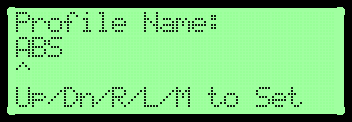
\includegraphics[]{profiles-name-01}
    \caption{Change Name}
  \label{fig:name}
\end{figure}

To change the letters, use the up and down keys.  To move between letters, use the left and right keys.  Press the center key to save all changes and return to the profile menu.  Note that if you are at the leftmost character (for example, the ``A'' in Figure~\ref{fig:name}) the left key will exit the menu without saving any changes.
\item Save to Profile:\label{sec:profiles-sp} selecting this saves your current home offsets and preheat settings to the selected profile and returns you to the ``Utilities'' menu.
\end{enumerate}

You can always save your current settings to a profile, replacing what is currently there.  This allows you to restore a profile, edit it in ``Preheat Settings'' (Section~\ref{sec:preheatset}) and ``Home Offsets'' (Section~\ref{sec:homeoff}) under the ``Utilities'' menu, and save it again.

\NextFile{ui-utilities-menu-home-offsets.html}

\subsection{Home Offsets} \label{sec:homeoff}
\index{Home offsets}
\index{Offsets!Home}
\index{Utilities!Home offsets}
\index{Menus!Home offsets}

This menu allows you to change the \glspl{home offset}, which define the center of the build plate (0,0,0) relative to the endstops.  For instance, if the X home offset is 152~mm, then the endstop is 152~mm to the right of the center.

This menu walks you through the three offsets, generating first the screen for the X offset (Figure~\ref{fig:xoff}).

 \begin{figure}[!htbp]
  \centering
    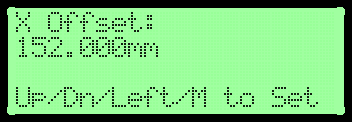
\includegraphics[]{offsets-01}
    \caption{X Offset}
  \label{fig:xoff}
\end{figure}

Pressing the up key increases the value, pressing the down key decreases the value.  The values are changed internally in units of steps and displayed to you in millimeters.  Press the left key to cancel any further changes, and the center key to confirm the change.  For example, if you only wish to adjust the X offset, press the center key to confirm the change for X and then press the left key to prevent any further changes.

\NextFile{ui-utilities-menu-toolhead-offsets.html}

\subsection{Toolhead Offsets} \label{sec:tooloff}
\index{Toolhead offsets}
\index{Offsets!Toolhead}
\index{Utilities!Toolhead offsets}
\index{Menus!Toolhead offsets}

This menu was added in Sailfish~7.7: you will not see it if you have an earlier version of Sailfish.  Additionally, this menu only appears for printers with an extruder count set to two as per Section~\ref{sec:extruder-count}.

With this menu, you can change the X and Y toolhead offsets which describe the spacing between the two extruder nozzles.  For a description of the toolhead offsets and how to calibrate them, see Section~\ref{sec:toolheadoffsets}.  Use of this menu is intended for when you wish to check the toolhead offsets or set their values in units of millimeters.  If instead you have printed the standard nozzle calibration print and are seeking to input the integer indices ranging from 1 to 13, then use the ``Calibrate Nozzles'' menu described in Section~\ref{sec:calibnozz}

The use and navigation of this menu is identical to that for the ``Home Offsets'' menu, with the exception that this menu only changes values for the X and Y axes.  See Section~\ref{sec:homeoff} for usage directions.

\NextFile{ui-utilities-menu-jog-mode.html}

\subsection{Jog Mode} \label{sec:jog}
\index{Jogging}
\index{Utilities!Jog}
\index{Menus!Jogging}

This menu allows you to move the extruder and build plate.  When selected, the jog X screen should be generated.  You can navigate between the jog X, Y, and Z screens with the left and right keys.  The jog Y screen is shown in Figure~\ref{fig:jog} below.

\begin{figure}[!htbp]
  \centering
    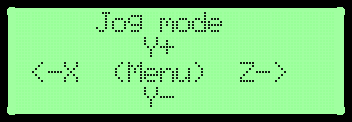
\includegraphics[]{jog-02}
    \caption{Jog Y}
  \label{fig:jog}
\end{figure}

As the screen shows, to increase the X, Y, or Z value press the up key, and press the down key to decrease the value.  The center key may be pressed to return you to the ``Utilities'' menu.  Note that +X is towards the right, +Y is towards the back, and +Z is towards the bottom.

\NextFile{ui-utilities-menu-enable-disable-steppers.html}

\subsection{Enable/Disable Steppers} \label{sec:steppers-enable}
\index{Stepper motors, enabling}
\index{Utilities!Enable steppers}
\index{Utilities!Disable steppers}

Selecting this will change the status of all stepper motors.  When they are enabled, they lock the axes in place.  Do not leave them enabled for extended periods of time as it heats up the motors needlessly.  By default, the stepper motors are disabled.

\NextFile{ui-utilities-menu-auto-level-variance.html}

\subsection{Auto-level Variance} \label{sec:alevel-variance}
\index{Auto-leveling!Max variance}

Firmware assisted auto-leveling support was introduced in Sailfish~7.7 and 4.7 for all printers equipped with ATmega 2560 microprocessors.  This parameter specifies the maximum tolerable difference in heights between the probing points.  If the difference in height between any two of the three probing points exceeds this parameter, then a print which attempts to enable auto-leveling will be canceled with the error message, ``Auto-level failed; too far out of level''.  Should that occur, it is time to manually relevel the build plate; see Section~\ref{sec:leveling}.

\begin{figure}[!htbp]
  \centering
    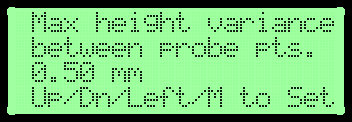
\includegraphics[]{alevel-01}
    \caption{Auto-level variance}
  \label{fig:alevel-variance}
\end{figure}

With this menu, depicted in Figure~\ref{fig:alevel-variance}, you can alter the value of this parameter.  The default value is 0.5~mm, and may be set to any value in the range 0.01 to 0.99~mm.  Pressing the up key increases the value, pressing the down key decreases the value.  Press the left key to cancel your changes; press the center key to confirm the change.

\NextFile{ui-utilities-menu-max-z-probe-hits.html}

\subsection{Max Z Probe Hits} \label{sec:alevel-maxhits}
\index{Auto-leveling!False probe hits}

When auto-leveling is active the Z height probe may be triggered by the ongoing build.  This might happen if over-extrusion is occurring, if the build has come loose, etc.  By default, the printer will initiate a pause and await user intervention when more than twenty triggers --- probe hits --- occur.  You may increase or decrease this value within the range of 1 to 200.  If you wish, you can disable this entirely by setting the ``max Z probe hits'' parameter to the value 0.  

\begin{figure}[!htbp]
  \centering
    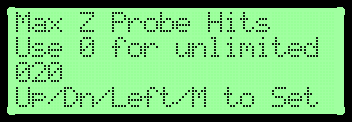
\includegraphics[]{alevel-02}
    \caption{Max Z probe hits}
  \label{fig:alevel-maxhits}
\end{figure}

To operate the menu, depicted in Figure~\ref{fig:alevel-maxhits}, press the up and down keys to increase or decrease the value.  To effect the change, press the center key.  To leave the menu without changing the setting, press the left key.

\NextFile{ui-utilities-menu-calibrate-nozzles.html}

\subsection{Calibrate Nozzles} \label{sec:calibnozz}
\index{Calibration!Dual extrusion|(}
This menu item is only available for printers with an extruder count set to two (see Section~\ref{sec:extruder-count}).

After you have run a nozzle calibration print, as described in Section~\ref{sec:dual-calib}, and having determined which of the thirteen X lines and which of the thirteen Y lines line up the best, this item allows you to enter their indices.  The firmware will take these indices and then compute and set the proper X and Y toolhead offsets.

It is important to note that \emph{these indices are not stored themselves}.  They are merely inputs used to compute the correct \emph{toolhead offsets} which \emph{are} stored.  Do not expect to return to this screen at a later date and see your values saved.  When you enter the screen you will always see the numbers 7 and 7, as they correspond to ideal nozzle spacings, as shown in Figure~\ref{fig:alignnozzles}.

\begin{figure}[!htbp]
  \centering
    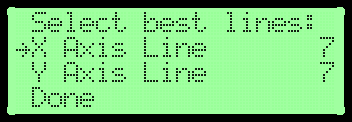
\includegraphics[]{align-01}
    \caption{Align Nozzles}
  \label{fig:alignnozzles}
\end{figure}

To change the values, press the center key to select the line and then use the up key to increase the value or the down key to decrease the value.  Note that the values range from one to thirteen and do not wrap.  Press the center key to save the change.  Either pressing the left key (when a line is not selected) or choosing the ``Done'' option returns you to the ``Utilities'' menu.
\index{Calibration!Dual extrusion|)}

\NextFile{ui-utilities-menu-restore-settings.html}

\subsection{Restore Settings} \label{sec:restore-settings}
\index{Utilities!Restore settings}
\index{Factory defaults}
\index{Resetting the printer}

Selecting this option will generate a confirmation screen, as depicted in Figure~\ref{fig:restore} below.  Confirming the change will restore all factory settings save for the home offsets and toolhead offsets (Sections~\ref{sec:homeoff} and \ref{sec:tooloff}).  This will also save lifetime filament and print hours information.  If you wish to reset everything, see Section \ref{sec:eeprom}.

\begin{figure}[!htbp]
  \centering
    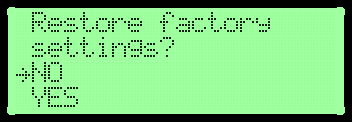
\includegraphics[]{restore-01}
    \caption{Restore Factory Settings}
  \label{fig:restore}
\end{figure}

\NextFile{ui-utilities-menu-eeprom.html}

\subsection{EEPROM} \label{sec:eeprom}
\index{Utilities!EEPROM}
\index{Menus!EEPROM}
\index{EEPROM}
\index{Resetting the printer}

\gls{EEPROM} stands for Electrically Erasable Programable Read-Only Memory.  Operational parameters for your printer, such as home offsets (Section~\ref{sec:homeoff}), preheat temperatures (Section~\ref{sec:preheatset}), etc.\ are saved in your EEPROM.\ \ Selecting this item generates a warning screen (Figure~\ref{fig:EEPROMwarning}), as, should you accidentally restore an EEPROM file from a different printer, you may make your printer inoperable.

\begin{figure}[!htbp]
  \centering
    
\includegraphics[]{eeprom-01}
    \caption{Use EEPROM With Care}
  \label{fig:EEPROMwarning}
\end{figure}

You may dismiss this screen by pressing the up key, which will generate the EEPROM menu, as shown in Figure~\ref{fig:eeprom}.  Pressing the left key will return you to the ``Utilities'' menu.

\begin{figure}[!htbp]
  \centering
    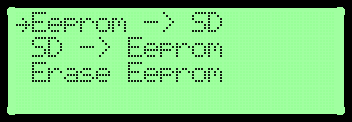
\includegraphics[]{eeprom-02}
    \caption{The EEPROM Menu}
  \label{fig:eeprom}
\end{figure}

This menu allows you to write your EEPROM to an SD card installed in your printer.  This creates a 4K file called \texttt{eeprom\textunderscore dump.bin} in the currently selected folder.\index{eeprom\textunderscore dump.bin@\texttt{eeprom\textunderscore dump.bin}}\index{EEPROM!Saving}  If this file already exists, an error message will be displayed and the transfer will not happen.  You may press the center key to dismiss the error message and return to the EEPROM menu.

The second item in the menu allows you to replace your EEPROM with the settings on your SD card (Figure \ref{fig:three}).  To successfully implement the settings on your SD card, you must press the center key a total of four times, at which point it will restore the file, and tell the printer to reset itself, returning you to the main menu, Section \ref{sec:Main}.\index{EEPROM!Restoring}

\begin{figure}[!htbp]
  \centering
    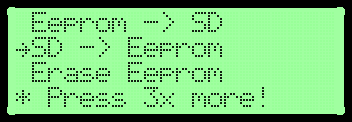
\includegraphics[]{eeprom-03}
    \caption{Due to the dangerous nature of restoring settings from an SD card, you are asked to confirm your selection of this item multiple times in order to prevent an accidental selection which may render your printer inoperable.}
  \label{fig:three}
\end{figure}

The final item in this menu (``Erase EEPROM'') will reinitialize the entire EEPROM memory.  Unlike the ``Restore Settings'' menu (Section~\ref{sec:restore-settings}), this item even resets the home and toolhead offsets, restoring \emph{all} factory defaults.

\NextFile{ui-utilities-menu-version-information.html}

\subsection{Version Information} \label{sec:versinf}
\index{Utilities!Version information}
\index{Screens!Version information}
\index{Version}
\index{Revision}
\index{Build date}

Selecting this item generates a screen similar to the one depicted in Figure~\ref{fig:vi}. 

\begin{figure}[!htbp]
  \centering
    \includegraphics[]{version-01}
    \caption{Version Information}
  \label{fig:vi}
\end{figure}

This contains the following information:

\begin{enumerate}
\item The type of machine for which the firmware was compiled.  Hopefully this corresponds to the type of your printer.
\item The amount of free bytes of memory (RAM) that your printer has.  If this gets below 50, something is wrong with the firmware.\index{Memory usage}
\item The \myhref{http://www.thingiverse.com/thing:32084}{Thingiverse ``Thing'' number 32084}.
\item The date the firmware was built in year/month/day format.
\item The version and revision numbers of the firmware.
\end{enumerate}


\NextFile{parameters.html}

\chapter{Firmware Parameters} \label{chap:firmware-settings}

Sailfish stores numerous firmware settings within your printer's EEPROM.  All of these parameters may be changed from your computer using ReplicatorG, MakerWare, or MakerBot Desktop.  On Replicator style printers, some of these parameters may also be changed from the front panel display described in Chapter~\ref{chap:whatever}.

\begin{itemize}
\item \textbf{MakerBot MakerWare:} see Section~\ref{sec:makerware} for instructions on configuring MakerWare to handle ``onboard parameters'' with Sailfish. Once the EEPROM maps are installed and Conveyor (background services) restarted, power on your printer and connect it to your computer via USB.  Access the printer's onboard parameters via the ``Machine'' menu.
\item \textbf{MakerBot Desktop:} Power on your printer and connect it to your computer via USB.  Access the printer's onboard parameters via the ``Onboard Preferences'' menu.
\item \textbf{ReplicatorG 40 -- Sailfish:} Be sure to use ``ReplicatorG 40 -- Sailfish'' (Section~\ref{sec:soft-reqs}).  If you have MakerWare or Desktop installed, you must first shut down Conveyor (Section~\ref{sec:conveyor}).  Before connecting to the printer over USB, select the correct machine type (Section~\ref{sec:machine-type}); then you may connect over USB, and invoke the ``Onboard Preferences'' (Section~\ref{sec:machine-type}).
\end{itemize}

Table~\ref{tab:def-params} lists the bulk of the firmware parameters, their default values, and the sections of this manual where information on them may be found.

{\def\NB{\textsuperscript{*}}
{\begin{table}[!hb]
\centering
\begin{tabular}{l | c | c c c }
\hline
\textbf{Parameter} & \textbf{Section} & \textbf{Replicators} & \textbf{Thing-o-Matics} & \textbf{Cupcakes} \\
\hline
acceleration & \ref{sec:acceleration-enable} & enabled & enabled & enabled \\
accel max X, Y\NB & \ref{sec:maxaccels} & 1000 mm/s\textsuperscript{2} & 500 mm/s\textsuperscript{2} & 500 mm/s\textsuperscript{2} \\
accel max Z\NB & \ref{sec:maxaccels} & 150 mm/s\textsuperscript{2} & 150 mm/s\textsuperscript{2} & 100 mm/s\textsuperscript{2} \\
accel max A, B\NB & \ref{sec:maxaccels} & 2000 mm/s\textsuperscript{2} & 10000 mm/s\textsuperscript{2} & 10000 mm/s\textsuperscript{2} \\
auto-level variance & \ref{sec:alevel-variance}, \ref{sec:alevel-params} & 0.50~mm & 0.50~mm & n/a \\
check SD reads & \ref{sec:sd-crc} & disabled & disabled & disabled \\
deprime A, B\NB & \ref{sec:deprime} & 16 steps & 8 steps & 20 steps \\
deprime on travel\NB & \ref{sec:deprime} & disabled & disabled & disabled \\
ditto printing & \ref{sec:ditto} & disabled & disabled & disabled \\
extruder count & \ref{sec:extruder-count} & varies & 1 & 1 \\
extruder hold & \ref{sec:extruder-hold} & disabled & disabled & enabled \\
HBP installed & \ref{sec:hbp-present} & varies & yes & no \\
home offset X & \ref{sec:homeoff}, \ref{sec:home-offsets} & Table \ref{tab:default-offsets} & none & none \\
home offset Y & \ref{sec:homeoff}, \ref{sec:home-offsets} & Table \ref{tab:default-offsets} & none & none \\
home offset Z & \ref{sec:homeoff}, \ref{sec:home-offsets} & Table \ref{tab:default-offsets} & none & none \\
JKN K\NB & \ref{sec:tuning-k} & 0.0050 & 0.0070 & 0.0085 \\
JKN K2\NB & \ref{sec:tuning-k2} & 0.0550 & 0.0040 & 0.0090 \\
override gcode temp & \ref{sec:override} & disabled & disabled & disabled \\
pause with heat & \ref{sec:pauseheat} & disabled & disabled & disabled \\
preheat temp extruder & \ref{sec:preheatset} & 230\,C & 220\,C & n/a \\
preheat temp HBP & \ref{sec:preheatset} & 100\,C & 110\,C & n/a \\
p-stop control & \ref{sec:pstop-enable} & disabled & disabled & disabled \\
RGB lighting\NB & \ref{sec:rgb-led} & white & white & white \\
slowdown\NB & \ref{sec:slowdown} & enabled & enabled & enabled \\
sound & \ref{sec:sound} & disabled & disabled & disabled \\
speed change max X, Y\NB & \ref{sec:maxspeedchanges} & 15 mm/s & 30 mm/s & 30 mm/s \\
speed change max Z\NB & \ref{sec:maxspeedchanges} & 10 mm/s & 10 mm/s & 25 mm/s \\
speed change max A, B\NB & \ref{sec:maxspeedchanges} & 20 mm/s & 30 mm/s & 30 mm/s \\
toolhead offset X & \ref{sec:tooloff}, \ref{sec:toolheadoffsets} & Table \ref{tab:default-offsets} & n/a & n/a \\
toolhead offset Y & \ref{sec:tooloff}, \ref{sec:toolheadoffsets} & Table \ref{tab:default-offsets} & n/a & n/a \\
Z probe hits & \ref{sec:alevel-maxhits}, \ref{sec:alevel-params} & 20 & 20 & n/a \\ [0.5ex]
\hline
\end{tabular}
\caption[Firmware parameters and their default values]{Firmware parameters and their default values.
\newline
\NB May only be changed with ReplicatorG, MakerWare, or MakerBot Desktop.}
\label{tab:def-params}
\end{table}}

\begin{table}[!ht]
\centering
\begin{tabular}{r | r r r | r r}
\hline
&\multicolumn{3}{c|}{\textbf{Home Offsets}}&\multicolumn{2}{c}{\textbf{Toolhead Offsets}} \\
\textbf{Printer}&\multicolumn{1}{c}{\textbf{X}}&\multicolumn{1}{c}{\textbf{Y}}&\multicolumn{1}{c|}{\textbf{Z}}&\multicolumn{1}{c}{\textbf{X}}&\multicolumn{1}{c}{\textbf{Y}} \\
\hline
Replicator 1& 152 mm & 75 mm & 0 mm & 33 mm & 0 mm \\
FlashForge Creator& 152 \hphantom{mm} & 75 \hphantom{mm} & 0 \hphantom{mm} & 34 \hphantom{mm} & 0 \hphantom{mm}  \\
WanHao Duplicator 4& 146.2 \hphantom{mm} & 73.5 \hphantom{mm} & 0 \hphantom{mm} & 33 \hphantom{mm} & 0 \hphantom{mm} \\
Replicator 2& 152 \hphantom{mm} & 75 \hphantom{mm} & 0 \hphantom{mm} &\multicolumn{1}{c}{n/a} & \multicolumn{1}{c}{n/a} \\
Replicator 2X& 152 \hphantom{mm} & 75 \hphantom{mm} & 0 \hphantom{mm} & 35 \hphantom{mm} & 0 \hphantom{mm} \\ [0.5ex]
\hline
\end{tabular}
\caption[Default home and toolhead offsets]{Default home and toolhead offsets}
\label{tab:default-offsets}
\end{table}}

\NextFile{parameters-home-offsets.html}

\section{Home Offsets} \label{sec:home-offsets}
\index{Home offsets|(}
\index{Offsets!Home|(}
\index{Parameters!Home offsets|(}

By convention, the center of the build platform is assumed to be the point (0,0,0) in XYZ space.  The X, Y, and Z \glspl{home offset} tell the printer the location of the X, Y, and Z endstops in relation to the build platform's center.\footnote{If your printer has a software-based auto-leveling feature, then the Z home offset may be used for different purporses.  See Section~\ref{sec:auto-leveling} for additional information.}  For instance, the typical Z home offset value is 0.0~mm.  This means that when the printer raises the platform until is activates the Z endstop --- that is, when it ``homes'' the Z axis --- it raises the build plate up to the extruder and then lowers it by the home offset value.

\begin{figure}[!htbp]
  \centering
    \ifpdf
       \includegraphics[width=5in]{home-offsets}
    \else
       \includegraphics[width=7in]{home-offsets}
    \fi
    \caption{Relationship between the build plate's center and the X \& Y home offsets}
  \label{fig:xy-home-offsets}
\end{figure}

Similarly, the X and Y home offsets tell the printer how far the endstops are from the center of the build platform, giving your printer a general ``sense'' of where it is so that it is able to accurately find the center of the build platform.   This relationship is depicted in  Figure~\ref{fig:xy-home-offsets}. This is important as the printer does not have sensors that tell it where the extruder or build platform are located.  When it begins a print, the printer ``homes'' the axes --- it moves the extruder along the X and Y axes until it hits the endstops and then it raises the platform along the Z axis until reaching that endstop.  Since the resulting position is well-defined, your printer tracks the movement of the plate and extruder so that it always ``knows'' where they are.  As this information is lost whenever you power cycle the printer, homing is a necessity at the start of every print.

The home offsets may be set from the printer's front panel as explained in Section~\ref{sec:homeoff}.  They may also be set from ReplicatorG, MakerWare, and MakerBot Desktop using the ``Machine'' menus and accessing the onboard parameters.

As most \glspl{slicer} center a print, if your prints do not appear well-centered then your home offsets are likely incorrect because they effectively define (0,0,0) for your printer.   To change the X offset, it is important to note that the X endstop is to the right of the center.  So, if prints are centered too far to the left, you should reduce the X home offset value.  Likewise, if the print is centered too far to the right, then increase the value.  If the prints are centered too far forward then decrease the value of the Y home offset; if the center needs to be moved forward, then increase the value.  Consult Table~\ref{tab:default-offsets} for a list of the default home offsets for many printers.  Note that Cupcakes and Thing-o-Matics do not have default values for their home offsets.  Owners of those two printers set their home offsets by running a calibration script such as that supplied with ReplicatorG.

\begin{bclogo}[logo=\bcinfo, noborder=true, couleurBarre=yellow]{Note}
If you have a dual extruder setup and printing with the left extruder seems off, then the problem is likely in the toolhead offsets, which are described in Section~\ref{sec:toolheadoffsets}.
\end{bclogo}

More care is needed in changing the Z home offset; if made too large, the nozzle and build plate can sustain damage.  Since the Z home offset describes the position of the nozzle in relation to the build plate after homing, increasing the offset tells the printer that the plate is farther from the nozzle than it might actually be.  For example, if you change the home offset value to 1.00~mm and the print begins at 0.15~mm (which is typical for models sliced at 0.30~mm layer height) then the printer will move the build plate up 0.85~mm.  Which, if the build plate was actually closer to the nozzle, can drive the plate into the nozzle.  For this reason, understanding, forethought, and planning are much more important in changing the Z offset value than the X and Y values.  A deeper discussion of the Z home offset may be found in Section~\ref{sec:z-home-offset}.

Note that you should be cautious and thoughtful in changing the Z home offset.  Nevertheless, here are two situations in which you may wish to change the Z home offset: if you have adhesion problems with the first layer of your print, then you may set the Z home offset to a value such as 0.05~mm, making the first layer of the print start 0.05~mm closer to the build plate than it would have otherwise; or, if the extruder is clicking a lot on the first layer since the nozzle is too close to the platform and the filament cannot exit it, then you might decrease the Z home offset to a value such as -0.03~mm.
\index{Home offsets|)}
\index{Offsets!Home|)}
\index{Parameters!Home offsets|)}

\NextFile{parameters-toolhead-offsets.html}

\section{Toolhead Offsets} \label{sec:toolheadoffsets}
\index{Toolhead offsets|(}
\index{Offsets!Toolhead|(}
\index{Parameters!Toolhead offsets|(}

The \glspl{toolhead offset} are only relevant to printers with two extruders.  If your printer has a single extruder setup, then ignore this section.

When, however, you have two extruders, the printer must know the spacing between the nozzles.  The reason being that, when the printer switches extruders, it needs to know what distance to move the extruder carriage so that, for example, the left extruder is now over the exact position at which the right extruder finished printing.  This spacing along the X and Y axes is known as the X and Y toolhead offsets.  It is assumed that the two nozzles are at the same Z position, and thus there is no Z toolhead offset.  Each printer manufacturer has an ``ideal'' set of nozzle spacings, which are built into each printer-specific version of Sailfish.  However, owing to manufacturing tolerances, your nozzles may not quite be spaced with the ideal offsets.  As differences of tenths of millimeters can impact the final appearance of your prints, you can adjust the toolhead offsets to match your printer.

These values may be set from the printer's front panel as explained in Section~\ref{sec:tooloff}.  They may also be set from ReplicatorG, MakerWare, and MakerBot Desktop using the ``Machine'' menus and accessing the onboard parameters.  However, there is a simpler method to set the toolhead offsets: print a calibration print.  Complete step-by-step directions may be found in Section~\ref{sec:dual-calib}.

Additional details on the implementation of toolhead offsets are given in Section~\ref{sec:toolhead-offsets-detail}.  Look to that section if you plan on making your own calibration prints and need to know, for instance, the sign conventions associated with application of the offsets.
\index{Toolhead offsets|)}
\index{Offsets!Toolhead|)}
\index{Parameters!Toolhead offsets|)}

\NextFile{parameters-acceleration.html}

\section{Acceleration}
\index{Acceleration|(}

The print files for any print include directions that determine the speed at which each line segment is printed.  As such, different portions of the print may print at different speeds, causing the printer to speed up or slow down as it transitions between speeds.  By default, when a change of speed is required, the printer effects the change by carefully accelerating to higher speeds or decelerating to lower speeds.  It is possible to turn off this feature by setting the acceleration parameter to ``off'' (Section \ref{sec:acceleration-enable}).  There is no practical reason to do this as printing with acceleration enabled --- the default --- results in smoother, quieter prints that obtain higher speeds.  Turning off acceleration when executing commands at speeds in excess of 30--40~mm/s may cause damage to your printer.
\index{Acceleration|)}

\NextFile{parameters-maximum-accelerations.html}

\subsection{Maximum Accelerations} \label{sec:maxaccels}
\index{Parameters!Maximum acceleration|(}

When acceleration is enabled, your printer needs to pick rates at which to accelerate or decelerate when transitioning between the commanded speeds in a print file.  The maximum acceleration parameters limit how quickly the transition can occur on each axis: X, Y, Z, A, and B.  Note that the A and B axes are the right and left extruders --- if you have only one extruder, then there is no B axis.

The maximum for an axis limits both the acceleration and deceleration with one value that is used for \emph{both}.  The default maximum acceleration values are listed in Table~\ref{tab:def-params}.

If your prints show noticeable overshoot at, say, 90\textdegree\ corners in cubes, then it may well be that your printer is attempting to decelerate faster than its mechanics actually allow.  \index{Print defects!Corner overshoot}The printer has no idea how fast it can really accelerate or decelerate --- it has no built-in feedback system to tell it when it overshoots.  As such, specific printers may need to have their maximum acceleration values changed.  For example, the defaults use the same value for both the X and Y axes.  But, in practice, many printers move far more mass around on their Y axis than their X axis.  With the added mass, the Y axis may not be able to accelerate or decelerate as fast as the X axis can.  Therefore, the maximum acceleration for the Y axis probably should not be the same as that for the X.\footnote{If you see overshoot at corners, it may also be a sign that you need to tune the JKN Advance parameters K or K2.  If the overshoot occurs even at moderate speeds, then see Chapter~\ref{chap:tuning}.}
\index{Parameters!Maximum acceleration|)}

\NextFile{parameters-maximum-speed-changes.html}

\subsection{Maximum Speed Changes} \label{sec:maxspeedchanges}
\index{Parameters!Maximum speed changes|(}

The maximum speed changes regulate the maximum instantaneous changes in speed the printer may effect in transitioning between speeds without carefully accelerating or decelerating through intermediate speeds.  This upper limit is imposed by the maximum X, Y, Z, A, and B speed changes as expressed in units of mm/s.  Note that, while high values can increase printer vibration and even cause it to jerk about, excessively low values significantly increase print times.  Refer to Table~\ref{tab:def-params} for a list of the default maximum speed changes.
\index{Parameters!Maximum speed changes|)}

\NextFile{parameters-auto-leveling.html}

\section{Auto-leveling} \label{sec:alevel-params}
\index{Parameters!Auto-leveling|(}

Some printers incorporate Z-probe mechanisms to measure the build plate position and automatically compensate the print level.  This is referred to as auto-leveling; support for it was introduced in Sailfish~7.7 and 4.7.  This support includes two firmware parameters.  The first, ``auto-level variance'' (Section \ref{sec:alevel-variance}) specifies just how out-of-level your build plate can be and still use auto-leveling.  If the difference in Z height between any two of the three probe points exceeds the variance parameter, then the print is cancelled and you are asked to manually relevel the build plate.\footnote{While the firmware could accommodate a very out-of-level build plate, there is little practical purpose to this.  Sailfish imposes a variance limit as this allows the use of an optimized algorithm for improved print speed.  While some firmwares do allow unlimited variance, this creates significant performance degradation regardless of how level the plate actually is.}  By default, this parameter is set to 0.5~mm.  Its permitted range is anywhere from 0.01~mm to 0.99~mm.  Note, however, that higher values may result in noticeable skew for taller prints if the build plate is uneven.

The second auto-leveling related parameter is the maximum number of probe hits which will be tolerated before the printer pauses and requests manual intervention (Section~\ref{sec:alevel-maxhits}). Set this parameter to the value 0 to ignore all probe hits once the print begins.  Otherwise, it may be set to any value in the range 1 -- 200.  The default value is 20, meaning that, on probe hit number 21, the printer pauses.  The count of hits is reset back to 0 after resuming the print.
\index{Parameters!Auto-leveling|)}

\NextFile{parameters-deprime.html}

\section{Firmware Retraction (Deprime)} \label{sec:deprime}
\index{Deprime}
\index{Deprime!On travel}
\index{Retraction, firmware}
\index{Parameters!Deprime|(}

This allows you to configure the printer with a filament retraction setting (in units of steps) to be used when pauses occur, planned or otherwise.  You are able to separately control the right extruder, A, and the left extruder, B.  If your printer is only equipped with one extruder, it is considered ``A''.

When a deprime setting is non-zero, the printer will deprime the associated extruder by the specified number of steps when it is active and any of the following occurs:

\begin{enumerate}
\item Pausing, whether user initiated or a P-Stop generated pause.
\item When the printing process is temporarily idle because the queue of processed segments has run out.  Depriming the active extruder will help prevent blemishes.
\item If ``Deprime on Travel'' is enabled, then, when the printer detects a \gls{travel move} it will deprime.  However, it is difficult for the printer to truly detect this, as the printing of very low layer heights may require many short printing moves which are not accompanied by extrusion.  In actuality, the printer can only identify travel moves if the print commands disable the extruder stepper motor before effecting a move.  Note that most slicers \emph{do not} disable the extruders before a travel move, as it may allow the filament to back out of the extruder by an unknown amount.
\end{enumerate}

When printing resumes, the printer then feeds the filament back in by the same number of steps by which it was deprimed.

By default ``Deprime on Travel'' is disabled, though deprime is set to a non-zero value for each extruder as per Table~\ref{tab:def-params}.
\index{Parameters!Deprime|)}

\NextFile{parameters-slowdown.html}

\section{Slowdown} \label{sec:slowdown}
\index{Parameters!Slowdown|(}

By default, this feature is enabled.  It makes the printer slow down when the queue of already processed line segments is running low.  By printing the remaining queued segments more slowly, there is more time for the queue to refill.  This helps prevent the printer sitting idle when the queue completely empties, eliminating the tiny blemishes that may form while plastic continues to ooze from the idle extruder.

Normally, the queue of processed line segments is full.  There are only two common situations in which the queue starts to run dry: first, when quickly printing many short line segments in small, fine detail;  second, when printing over a serial USB connection where the computer sending the data over the USB is slow.

There is no practical reason to disable this option other than to see the effects of printing small fine detail quickly (120~mm/s) without it enabled.
\index{Parameters!Slowdown|)}

\NextFile{parameters-rgb-led.html}

\section{Lighting (RGB LED)} \label{sec:rgb-led}
\index{RGB LED lighting}
\index{Lighting}
\index{Parameters!RGB LED|(}

Some printers come equipped with RGB LED lighting strips to light the printing bay.  The printer controls this lighting, and sets the colors which appear.  The settings for these lighting strips may only be controlled from your computer, most comfortably from ReplicatorG's ``Onboard Preferences'' window, accessed from its ``Machine'' menu.  MakerWare and Desktop may also be used, but not as conveniently.

Three aspects of the lighting may be controlled:

\begin{enumerate}
\item The choice of color: white (0), red (1), orange (2), pink (3), green (4), blue (5), purple (6), off (7), and custom (8).  The default selection is white. Use ``off'' (7) to turn the lighting off.  When using MakerWare or Desktop, you will need to use the listed numeric values with the ``Basic Color'' setting.
\item A custom color will be used when you set the color choice to ``custom'' (8).  When using ReplicatorG, a ``color picker'' allows selection of a color from a palette.  From MakerWare and Desktop, you must provide an RGB value as three integers, each in the range 0 -- 255.
\item You can elect to have the lighting cycle from blue (cool) to red (hot) as each heater heats up.  Once heating is complete and the printer begins printing, the lighting switches back to the normal color choice that has been set (or white if none has been set). In MakerWare and Desktop this appears as the option ``Led Heat''.  In ReplicatorG, this is the ``show heating progress by changing the lighting color'' checkbox.
\end{enumerate}
\index{Parameters!RGB LED|)}


\NextFile{tuning.html}

\chapter{Printer Calibration} \label{chap:tuning}

To get the best quality prints from your printer, you should invest some time in calibrating your slicing profiles to your printer.  Also, if you have a printer with two extruders, you should calibrate your \glspl{toolhead offset} so as to ensure good alignment in prints which use both extruders.

\NextFile{tuning-slicer-calibration.html}

\section{Slicer Calibration}
\index{Calibration!Slicing profile}

To get top quality prints, you will need to invest some time in calibrating
your \glspl{slicing profile} to suit both your printer and choice of filaments.
Fortunately, the process (presented in Section~\ref{sec:cube}) is simple and straightforward, though it does require a basic understanding of your slicing software.

%The overwhelming majority of users need only perform a basic calibration
%with the ``calibration cube''.  This is presented in Section~\ref{sec:cube}.
%Some users may be interested in also adjusting the JKN ``K'' and ``K2''
%parameters.  However, the default settings found in your printer are likely
%quite good already and not in need of any changes.

\NextFile{tuning-slicer-calibration-filament-diameter.html}

\subsection{Filament Diameter}
\index{Under-extrusion}
\index{Over-extrusion}

The need to measure your filament diameter before preparing a model for
printing \emph{cannot be stressed enough}.  It is important that you have use
of a caliper with which to measure the diameter of your filament.\footnote{A
digital caliper is easiest to use although a dial or vernier caliper will
work just as well.  You will need to produce measurements in units of
millimeters, mm.  Consequently, calipers which directly read in those units
is preferred.  Otherwise, you will need to convert to units of mm.}  Filament
sold as 1.75~mm filament may in fact be 1.68 or 1.85~mm in diameter.  However,
when preparing models for printing, especially large models,
it is critical that the slicing process know the actual diameter of the
filament.  Otherwise too much or too little filament will be extruded, as
the slicer determines the amount of filament needed based upon the
expected volume per millimeter of raw input filament.  If the actual diameter is
larger than expected, too much plastic will be extruded and
``\gls{over-extrusion}'' results.  And, if the diameter is smaller than
expected, too little plastic will be extruded and ``\gls{under-extrusion}''
results.

With a calibrated slicing profile and measured filament diameter, very
smooth top surfaces can be achieved when printing.  The blue tag print of
Figure~\ref{fig:smooth-top} is such an example.

\begin{figure}[!htbp]
  \centering
    \includegraphics[width=4in]{smooth-top}
    \caption{Smooth surface finish achieved through careful calibration and measurement}
  \label{fig:smooth-top}
\end{figure}

Over and under-extrusion has a cumulative effect: it will not impact small
models nearly as much as it will large models, which may fail to properly print.  Over-extrusion can jam the extruder when the buildup of plastic becomes so much that there is no longer a small gap
between the nozzle and the previously printed layer.  A printed model with
a deficit of plastic --- under-extrusion --- may be too weak to serve
its intended purpose.  Indeed, it may even break apart while being printed
or removed from the build plate.

\NextFile{tuning-slicer-calibration-usb-vs-sd.html}

\subsection{USB vs. SD Card}

If possible, prints should always be run from an SD card.  Printing
over USB introduces additional sources of problems and may result in
prints with small bumps.  \index{Print defects! USB}Accelerated printing runs fast enough that,
if your computer is busy with other tasks, there may occasionally be
small delays introduced to the serial communications.  These delays
can cause the printer to pause for very brief periods of time and
produce small bumps or blemishes --- the result of filament oozing out
of the idle extruder.\footnote{If the computer is not sending commands over USB to the printer, then even features such as deprime (Section \ref{sec:deprime}) and slowdown (Section \ref{sec:slowdown}) will not help prevent the formation of blemishes.}

When calibrating your printer, avoid this additional complication and print
from an SD card.  If you are ever printing over USB and see printing defects
you do not expect, then attempt the same print from an SD card and see
if that leads to an improvement.

\NextFile{tuning-slicer-calibration-know-your-defects.html}

\subsection{Know Your Defects}

Before launching into a discussion of tuning, you should first be
familiar with three particular print defects which, incidentally,
occur with or without accelerated printing and are not unique to Sailfish.  There are other defects as
well, but familiarity with these three is helpful as they may appear on
your calibration boxes.  You may not be used to seeing them when
printing at low speeds (e.g., 40~mm/s), but at higher speeds,
accelerated or otherwise, they will be more likely to manifest.

\subsubsection{Infill telegraphing} \label{sec:telegraphing}
\index{Telegraphing}
\index{Print defects!Telegraphing}

\Gls{infill} \gls{telegraphing}, such as that seen in
Figure~\ref{fig:telegraphing},
often occurs when printing with a single \gls{shell} and under-extruding.
It may also be caused by a hot extruder nozzle dragging over or pushing
into the layer below it, as can occur when over-extruding.  Make sure
that you correctly measured the filament diameter and supplied that value to your
slicer when slicing.  Also, be sure to calibrate your extruder as outlined in
Section~\ref{sec:cube}.

\begin{figure}[!htbp]
  \centering
    \includegraphics[width=3in]{telegraphing}
    \caption{Infill telegraphing through the print's perimeter}
  \label{fig:telegraphing}
\end{figure}

Any overshoot caused during infill direction changes may also cause this effect, in which case an extra
shell will help hide it. If excess momentum is implicated, then the
same techniques used to reduce corner ringing
(Section~\ref{sec:ringing}), may also be applied here.

A short term fix may be to slice your model with an additional shell or two.

Note that Figure \ref{fig:telegraphing} is an extreme case --- to the point where the
infill itself is visible between some of the perimeter's layers. On
some of the layers where the infill is not directly visible, ripples caused by
it or the nozzle pushing against the inside of the perimeter may still be
visible.

\subsubsection{Ringing} \label{sec:ringing}
\index{Ringing}
\index{Corner ringing}
\index{Print defects!Ringing}

At higher print speeds, when the motion of the build platform or
extruder makes a sudden change in direction, a ringing vibration may
occur.\footnote{In severe cases, there may be actual overshoot caused
by the extruder carriage's momentum carrying it farther than intended.
At issue is that the printer has no feedback mechanism and thus
does not know whether the maximum rates of acceleration and deceleration with which it
has been configured are actually achievable.}  Since
sudden direction changes are often associated with turning a corner in
the print, this effect is often referred to as ``\gls{corner
ringing}''.

\begin{figure}[!htbp]
  \centering
    \includegraphics[width=3in]{corner-ringing}
    \caption{Ripples caused by ringing}
  \label{fig:ringing}
\end{figure}

Although quickly dampened, this ringing nonetheless impacts surface
finish, as can be seen in Figure~\ref{fig:ringing}. Ringing is
particularly noticeable on long, flat surfaces and appears as ripples
which rapidly diminish in amplitude. Like infill telegraphing, this
can occur with non-accelerated printing as well as accelerated
printing. The advantage of accelerated printing is that acceleration
can be used to mitigate the issue while still attaining high print
speeds away from corners by lowering the maximum X and Y speed change
values, the maximum X and Y accelerations, or any combination of the
two. For non-accelerated printing, the only recourse is to print the
entire model at slower speeds.

Also note that the mechanics of a given printer may contribute to ringing
effects.  If you are experiencing problems with ringing, then research
postings about ringing in online forums and newsgroups relevant to your
make of printer.  You can also try rotating your model 45\textdegree\ before slicing.

\subsubsection{Stepper clipping} \label{src:clipping}
\index{Stepper clipping}
\index{Print defects!Stepper clipping}

When infill telegraphing and corner ringing are not present, you may
see some very faint rippling along flat faces when you look carefully
in the right lighting and from the right angle.  Figure~\ref{fig:clipping}
shows a print done on a Thing-o-Matic in ABS plastic which illustrates
this effect.

\begin{figure}[!htbp]
  \centering
    \includegraphics[width=3in]{clipping}
    \caption{Faint ripples caused by stepper clipping}
  \label{fig:clipping}
\end{figure}

This faint rippling may be caused by clipping of the sinusoidal control
signals to the stepper
motors.  Thing-o-Matics and Cupcakes with stepper motors from before
May 2011 are especially vulnerable to this issue.  Unfortunately, later
models suffer as well, as evidenced by the model shown in Figure \ref{fig:clipping} which was
produced on a Thing-o-Matic with post May 2011 stepper motors. Ed
Nisley described and analyzed this in his May 2011 blog posting,
\myhref{http://softsolder.com/2011/05/05/thing-o-matic-mbi-stepper-motor-analysis/}{Thing-o-Matic: MBI Stepper Motor Analysis}, found
at softsolder.com.  At low speeds, this clipping produces a faint
repeating pattern of about 25~Hz. At much higher stepper speeds, the pattern
has a frequency of 50~Hz. Hardware replacement is needed to nearly
eliminate the problem: stepper motors with winding resistances at or
below 2~Ohms, sufficient pull in torque, sufficiently low inductance,
and stepper drivers capable of handling the motors (e.g.,
Pololu).

Significantly slowing down the exterior printing speed may help mitigate
the effects of stepper clipping.  On well-designed and tuned printers,
this is often the one remaining print quality issue.  On suboptimal
or untuned printers, it is still present but hidden by more visible
printing defects.

\NextFile{tuning-slicer-calibration-box.html}

\subsection{Calibration Box} \label{sec:cube}
\index{Calibration!Box|(}

To achieve quality prints, start by ensuring that you can print a decent
calibration ``box'' whose top is nice and flat.  Producing a respectable box
involves calibrating a slicing profile to your printer and choice of
filaments.  So, until you can print a good calibration box, there is little
point in worrying about other printing defects you may be
experiencing.  Here is the step-by-step procedure for
accomplishing this calibration:

\begin{enumerate}

\item Obtain a model for a 10~mm high box which is 20~mm on a side.  ReplicatorG contains as its first example this calibration box:
look under the Examples section of the File menu.  It is the
{\smaller\texttt{20mm\textunderscore Calibration\textunderscore Box.stl}}.
Alternatively, \myhref{http://www.thingiverse.com/thing:2064}{Thing~\#2064} at thingiverse.com contains the calibration box as the download file {\smaller\texttt{20mmbox.stl}}.

\item Use calipers to measure the diameter of the filament with which you will be printing.

\item With the calibration box model in your slicer, slice it at a 0.3~mm
layer height, 100\% infill, and using the diameter of the filament you just
measured.\footnote{If using ReplicatorG with Skeinforge-50,
then do \emph{not} use hexagonal infill.   There is a bug in SF-50's hexagonal
infill which will result in irregular infill; use grid rectangular or line infill instead}  It is critical that you use
100\% infill and that you measure the diameter of your filament and input that
to the slicer.

\item Print the box.

\item Carefully examine the top surface of the box.  While it is easy to
see if the top is convex, you may need to use a
straight edge to gauge how flat or concave the top is.

\begin{enumerate}
\item If it is nice and flat, then you are done!
\item If it is convex, then
too much plastic was extruded and your printer is over-extruding.
Configure your slicing profile to put out slightly less plastic.  How you will do
this depends upon which slicer you use. For ReplicatorG, increase the 
``filament packing density'' in the Dimension plugin.  For MakerBot MakerWare
and Desktop, increase the ``feedstockMultiplier''.  For Simplify3D, reduce the
``extrusion multiplier''.  Only change the value in small increments, such as 0.05.
\item If it is slightly hollow (concave), then too little plastic was
extruded: your printer is under-extruding.  Decrease the filament packing
density (ReplicatorG), decrease the feedstockMultiplier (MakerWare and Desktop),
or increase the extrusion multiplier (Simplify3D).
\end{enumerate}

\item Go back to Step 3, reslicing, reprinting, and re-evaluating the result.
\end{enumerate}

If you happen to have two extruders, it is recommended to do this
calibration once for each extruder.  Then keep distinct slicing
profiles for each extruder: one for the right extruder and another
for the left extruder.

Once you can print a nice calibration box, you are ready to get back
to printing.  Keep in mind that this calibration process
should be repeated for different type of plastics.  At issue is the
differing hardnesses of the plastics used.  The pinch gear in your
printer's extruder feed mechanism bites into the plastic filament.
The depth to which it bites depends upon the hardness of the plastic.
And the deeper the bite, the smaller the effective turning radius of
the gear.  With smaller turning radius, less filament is fed per
rotation of the extruder stepper motor.  This calibration is primarily to address your extruder's handling of these variations in hardness.  For example, ABS is
significantly softer than PLA and so significantly different
adjustments may be needed for ABS versus PLA.  This will, of course,
depend upon the geometry of the pinch gear and how capable it is of
biting into the filament.
\index{Calibration!Box|)}

\NextFile{tuning-dual-extruder-calibration.html}

\section{Dual Extruder Calibration} \label{sec:dual-calib}
\index{Offsets!Toolhead}
\index{Toolhead offsets}
\index{Toolhead offsets!Calibrating|(}
\index{Calibration!Dual extrusion|(}

If your printer has only a single extruder, or if you never use two extruders for the same print, then you can skip this section.

When printing with both extruders, optimal print quality is achieved by precisely calibrating the distance between the two extruder nozzles.  As explained in Section~\ref{sec:toolheadoffsets}, this calibration information is stored as the ``toolhead offsets''.  In this section, a method of determining the toolhead offsets is presented. For every major type of printer, there is a nozzle calibration print in ``ReplicatorG 40 -- Sailfish'', that may be printed as described and then the results supplied to your printer.  Using the results of your print, your printer will then set the correct values for the toolhead offsets.

\begin{enumerate}
\item Before you begin, ensure that you have the latest Replicator G 40 -- Sailfish downloaded from the \myhref{http://www.thingiverse.com/thing:32084}{Sailfish ``Thing'' at Thingiverse}.
\item Launch ReplicatorG and select the correct machine type under the ``Machine Type'' item of the ``Machine'' menu.  Be sure that the machine type name includes ``(Sailfish)'' in it.  Figure~\ref{fig:repg-driver-2} shows The Replicator Dual (Sailfish) selected.

\begin{figure}[!htbp]
  \centering
    \includegraphics[width=5in]{repg-driver}
    \caption{Machine Type}
  \label{fig:repg-driver-2}
\end{figure}

\item Connect to your printer over USB (see Figure~\ref{fig:repgconnect}), then invoke the \Gls{onboard parameters} window with the ``Onboard Parameters'' item of the ``Machine'' menu.

\begin{figure}[!htbp]
  \centering
    \includegraphics[width=5in]{repg-connect}
    \caption{Connecting to Your Printer}
  \label{fig:repgconnect}
\end{figure}

\item In the ``Homing/VREFs'' tab, set the X and Y toolhead offsets to 0.0~mm.  Be sure to change the toolhead offsets and \emph{not} the home offsets (Figure~\ref{fig:tool-head-settings}).  Make sure to commit the change.  Note that resetting the printer to factory defaults will \emph{not} reset the X and Y toolhead offsets.

\begin{figure}[!htbp]
  \centering
    \includegraphics[width=5in]{tool-head-settings}
    \caption{Toolhead Offsets}
  \label{fig:tool-head-settings}
\end{figure}

\item To print the nozzle calibration print go to the ``Scripts'' item of the ``File'' menu, choose your printer type, and then select the ``Dual~Nozzle~Calibration.gcode'' item (Figure~\ref{fig:nozzle-calibration-script}).  Select the Replicator 1 if you do not see your printer type listed.  Note that the name may be an elongated version of this such as ``Flashforge~Creator~Dual~Nozzle~Calibration.gcode''.  Regardless, selecting this will bring up the \gls{gcode} file in ReplicatorG which you should then print to your printer.

\begin{figure}[!htbp]
  \centering
    \includegraphics[width=5in]{nozzle-calibration-script}
    \caption{Nozzle Calibration Menu}
  \label{fig:nozzle-calibration-script}
\end{figure}

\item Once the print is finished, you will see a series of horizontal line pairs running vertically up the left side of the build plate (Figure~\ref{fig:nozzle-calibration-print}).  Each pair of lines was printed using both extruders, and is numbered with a value between 1 to 13.  Line 1 is at the front of the plate and should be the longest.  Identify the pair for which each line is vertically the best aligned.  Remember this number.  In the example print of Figure~\ref{fig:nozzle-calibration-print}, either lines 1 or 2 seem to have the best alignment.

\begin{figure}[!htbp]
  \centering
\ifpdf
    \includegraphics[width=5in]{nozzle-calibration-print}
\else
    \includegraphics[width=8in]{nozzle-calibration-print}
\fi
    \caption{Nozzle Calibration Print}
  \label{fig:nozzle-calibration-print}
\end{figure}

\item The print will also have a series of vertical line pairs running horizontally across the front of the build plate.  Again, each pair of lines was printed with both extruders, and are numbered 1 to 13.  Line 1 is the leftmost and should also be the longest.  Identify which pair has the best alignment --- which pair has the middle ends closest horizontally.  Remember this number.  In the example print of Figure~\ref{fig:nozzle-calibration-print}, pair 6 appears best aligned.

\item On the printer's LCD screen navigate to the ``Calibrate Nozzles'' item under the ``Utilities'' menu (Section~\ref{sec:calibnozz}).  For the X and Y values, input the numbers you recorded for steps 7 and 6, respectively.  Then select the ``Done'' item on the fourth line of the screen.

\item Your toolhead offsets have now been set.  The values in ReplicatorG's Onboard Preferences will have changed unless you entered 7 for both X and Y, as Line 7 represents the ideal offset of 0.0~mm.  The actual lines are offset by by -0.6~mm, -0.5~mm, ..., 0.0~mm, 0.1~mm, ..., 0.6~mm, creating thirteen offsets total.
\end{enumerate}

Note, however, that, should you revisit the Calibrate Nozzles item on your printer, you will \emph{not} see the X and Y values you entered, as the printer does not save these values but instead uses them to recalibrate.  It is worth mentioning that, after recalibration, these values are no longer correct: if you were to reprint the nozzle calibration print, you should now find that Line 7 is the best match for both X and Y.
\index{Toolhead offsets!Calibrating|)}
\index{Calibration!Dual extrusion|)}

\NextFile{tuning-jkn-advance.html}

\section{JKN Advance K} \label{sec:tuning-k}
\index{JKN Advance!K}
\index{Advance|see{JKN Advance}}

The Jetty-Kubicek-Newman (JKN) Advance parameters address extrusion
issues associated with accelerating and decelerating molten plastic
through the extruder. Left uncorrected, these issues can
result in excess plastic at points of low speed (blobbing) as well as
small bumps (blemishes) and small gaps. In truth, some of these issues
are best addressed by using an ac\-cel\-er\-a\-tion-aware slicer or gcode post-processor. However, at present no such tools exist.

The first of the two JKN Advance parameters, K, addresses an issue
associated with a plastic deficit when accelerating and a plastic
surplus when decelerating. You will find a suitable value for K by
looking at the corners of your calibration boxes printed with
acceleration enabled and at reasonably fast speeds. The fill need
not be solid. Indeed, printing with 20\% infill will also be
informative --- make sure that it still looks good.

\begin{bclogo}[logo=\bcinfo, noborder=true, couleurBarre=yellow]{Important}
Before proceeding and expending time and effort, realize that your printer
ships with reasonably well-tuned JKN parameters.  If you are experiencing
printing defects, adjustment of these parameters will likely not be
satisfactory nor resolve any issues you are attempting to address.  The
following tuning information is more here to satisfy the curiosity of idle, technical minds.
\end{bclogo}

Begin calibrating K by ensuring that acceleration is enabled and
that the JKN Advance K2 parameter is set to 0 (Section \ref{sec:tuning-k2}).
Also, make sure that the maximum X and Y axes acceleration values
are at or below 500~mm/s\textsuperscript{2} so as to minimize overshoot effects.  These values may only be set with ReplicatorG -- Sailfish, MakerWare, or Desktop.  To use the latter two, refer to Section \ref{sec:makerware}.

Print a calibration box (Section~\ref{sec:cube}) with the default K
value of 0.005 (Replicator-style printer) or 0.007 (Thing-o-Matic or
Cupcake). Then print two more boxes, one with K set to 0.0025 and
another at 0.0075 (Replicator-style) or 0.005 and 0.009 (Thing-o-Matic
or Cupcake). It can also be helpful to print a calibration box with K set to 0
for comparison.

What you are looking for is a value of K which helps reduce the amount
of extra plastic at the corners but does not reduce it so much that the
corners become bevelled (i.e., foreshortened) or gaps begin appearing
in the solid surface layers (e.g., the box's top face). As you
decrease K below the optimal value, the top infill will be fine but the
extra plastic at the corners will begin to increase.

Keep in mind that there is no single ``ideal'' value for K. You just want to
get it into the right range.

\begin{figure}[!htbp]
  \centering
    \ifpdf
      \includegraphics[width=5in]{jkn-advance-k}
    \else
      \includegraphics{jkn-advance-k}
    \fi
    \caption{Calibrating JKN Advance K --- calibration boxes printed on a Thing-o-Matic with ABS plastic}
  \label{fig:jkn-advance-k}
\end{figure}

Examine the three calibration boxes shown in Figure~\ref{fig:jkn-advance-k}.  As you can see, the box
on the right with K=0.01000 is showing some gaps, so the value of K is
too large. The middle box with K=0.00500 has a reasonable top surface but
the corners might do with a little less plastic, so K is too small. The leftmost box, K=0.00250 could stand to have a better top surface, again, K is too small. For Thing-o-Matics with an Mk7 extruder, a better value of
K probably exists between 0.00500 and 0.01000.  Note that the firmware's
default value for Thing-o-Matics is 0.00850.  A different default value for
K is used on Replicator-style printers since they use a different extruder and
{\relsize{+1}\textfrac{1}{16}} microstepping --- compared the
Thing-o-Matic's {\relsize{+1}\textfrac{1}{8}}.

\NextFile{tuning-jkn-advance2.html}

\section{JKN Advance K2} \label{sec:tuning-k2}
\index{JKN Advance!K2}

The JKN Advance K2 parameter further corrects for o\-ver-pres\-sur\-i\-za\-tion
in the extruder during the deceleration phase. This is because the
pressurization during the acceleration phase and the depressurization
during the deceleration phase are not symmetrical in effect.

JKN Advance K2 is used to reduce blobbing and splaying in the corners
of boxes and at sharp angles between line segments.

To tune this value, begin by tuning JKN Advance K first as per
Section~\ref{sec:tuning-k}.  When tuning K2, leave K set to the value you
arrived at from that step: do not set K to zero when tuning K2 unless
you found zero to be the best choice for K.

Start by printing a calibration box with K2 set to 0 and 100\%
infill.  Look at the corners: you will see they protrude in the
direction of the filament travel. Increase K2 in units of 0.001 and
check again. Keep increasing JKN Advance K2 in units of 0.001 until
the corners are pulled in as much as possible.

When JKN Advance K2 is set too high, you will begin to see breakup in the top
surface of the box.

Note that the firmware's default value is 0.055 (Replicator-style
printers) and 0.004 (Thing-o-Matic, Cupcake).

\begin{figure}[!htbp]
  \centering
    \ifpdf
      \includegraphics[width=5in]{jkn-advance-k2}
    \else
      \includegraphics{jkn-advance-k2}
    \fi
    \caption{Calibrating JKN Advance K2 --- calibration boxes printed on a Thing-o-Matic with ABS plastic}
  \label{fig:jkn-advance-k2}
\end{figure}

All four boxes shown in Figure~\ref{fig:jkn-advance-k2} have
K=0.00850, the default value for K on a Thing-o-Matic. The
leftmost box, K2=0.0000, shows the corners when K2 is not
applied. The second box with K2=0.0050 shows a little improvement
with the two upper corners not projecting quite as much. The third
box with K2=0.0100 is just beginning to show some of the infill
plastic pulling away from the perimeter loops. This is quite
noticeable for the final box with K2=0.0300. A good value of K2 is
likely to be found between K2=0.0050 and K2=0.0100. Note that the
differences will be more noticeable to you when you have actual boxes
in your hands which you can look at from all angles. The pictures here
do not fully illustrate the effect of K2 on the prints.


\NextFile{install.html}

\chapter{Installing Sailfish} \label{chap:install}
\index{Installing}
\index{Firmware!Installing}

This details the installation of Sailfish on a printer currently running \gls{firmware} other than Sailfish.  If your printer already has Sailfish installed, instead refer to Chapter~\ref{chap:update}.

It is important to note that if your printer is new to you, then you are advised to consider using it for at least a week before switching firmware.  This allows you to get to know your printer and ensure that it is operating correctly before upgrading it in any way.  If you upgrade a new printer before establishing that it is functioning properly, it may be difficult to distinguish between manufacturing defects and changes introduced by the modifications you have created.  Do yourself a favor and take things \textsl{s\,l\,o\,w\,l\,y}.

If you are unsure what firmware your printer is running, these steps can help you ascertain the firmware type.\index{Identifying firmware}\index{Firmware!Identifying}

\begin{enumerate}
\item If your printer does not have an LCD display, you will need to connect
  directly to it over USB and find what firmware version it reports.
  If it reports a firmware version of 3.1 or earlier, then it is running MakerBot's 
  stock firmware.  A firmware version of 3.2 or later means that it is running 
  either the Jetty Firmware, 3.2--3.5, or Sailfish, 4.0 and later.  (The Jetty Firmware is Sailfish
  by an earlier name.)  If the latter is the case, see Chapter~\ref{chap:update} for information
  on upgrading your printer's firmware.
\item If your printer does have an LCD display, then turn it on.  As it powers
  up, watch the LCD display for a ``splash'' screen which will appear only
  for a few seconds.  If Sailfish is running on your printer, then the splash
  screen should be similar to that shown in Figure~\ref{fig:splash}.  Look
  to see if the word ``Sailfish'' appears.  If it does, then your printer is
  already running Sailfish and you should turn to Chapter~\ref{chap:update}.
  Even if the word ``Sailfish'' does not appear, it is still possible that you
  are already running Sailfish, as some manufacturers alter the splash screen to
  show different information.
\item If you missed seeing the splash screen or are still unsure what firmware 
  you are running, check and see how many top-level menu items your printer 
  has.  Sailfish only has the three presented in Section~\ref{sec:Main}. 
  However, this is not definitive as early versions 
  of MakerBot's firmware display only three top-level menu items as well.  
  But, if you see more than three top level menu selections, as well as the printer 
  name which appears on the first line, then you are unlikely to be running Sailfish.
\item Finally, go to the ``Version Information'' item of the
  ``Utilities'' menu and see what is displayed.  Refer to
  Section~\ref{sec:versinf} for samples of the Sailfish version
  information screen.  If you do not see the word ``Sailfish'' in the
  display, then you are not running Sailfish.
\end{enumerate}

Once you are satisfied that your printer is \emph{not} running Sailfish
\emph{and} you are ready to upgrade to Sailfish, then read on.  But please
follow these directions carefully so as to prevent any surprises that may delay
your return to printing.

\begin{bclogo}[logo=\bcinfo, noborder=true, couleurBarre=yellow]{Note}
On Replicator series printers, the Sailfish version numbers begin at 6.2.
On Thing-o-Matic and Cupcake printers, Sailfish version numbers begin at 4.0.
\end{bclogo}

\NextFile{install-hardware-reqs.html}

\section{Hardware Requirements}
\index{Requirements!Hardware}

Sailfish runs on \gls{MightyBoard} rev~E, G \& H as well as \gls{Gen 3} and
\gls{Gen 4} electronics.\index{MightyBoard}\index{Gen 3}\index{Gen 4}
For all Replicators, both single and dual extrusion is supported.  Specific per
machine requirements are as detailed below.  Note that each printer category
also supports the clones of the printers listed in that category.  For instance, The
Replicator 1 includes CTC, FlashForge, MBot3D, WanHao, ZYYX, and
other Replicator 1 ``clone'' printers.

\begin{enumerate}
\item \strong{The Replicator 2 and 2X:} MakerBot MightyBoard rev~G or H
electronics with one or two extruders.
\item \strong{The Replicator 1:} MakerBot MightyBoard rev~E electronics with
  one or two extruders.
\item \strong{Thing-o-Matics:} MakerBot v2.X motherboard, MakerBot v3.6
Extruder Controller, MakerBot v3.3 Step\-per Dri\-vers, a stepper-based extruder,
and an Arduino Mega or Arduino Mega 2560. Other than the extruder, these are
all ``stock'' Thing-o-Matic electronics; i.e., Gen 4 electronics. Stepper-based
extruders include the Mk6, Mk6+, Mk7, and Mk8.  Other electronics and extruders
may or may not work with the Sailfish firmware.
\item \strong{Cupcakes with Gen 4 electronics:} As per the requirements for
  Thing-o-Matics.
\item \strong{Cupcakes with Gen 3 electronics:} Stepper motor extruder plus
 the 3G5D Shield or the ``Ugly Cable Hack'' to control the stepper motor
 extruder.  Additionally, the remaining complement of Gen 3 electronics: RepRap
 Motherboard v1.2, Plastruder Extruder Controller, and v2.3 or later stepper
 drivers.\index{3G5D shield}\index{Ugly cable hack}
\end{enumerate}

If your printer does not satisfy the above requirements, then Sailfish
likely will not run on it.  For example, Sailfish does not presently
support RAMBo, RAMPS, or other common RepRap electronics.

\NextFile{install-hardware-reqs-cupcakes-and-thingomatics.html}

\subsection{Cupcakes and Thing-o-Matics}

If you are using a Cupcake or Thing-o-Matic, you must know the type of
motherboard that you have.  For Gen~4 electronics, this will be an Arduino Mega
or Arduino Mega 2560 and will appear in ReplicatorG's Firmware Upgrade
window as ``MakerBot Thing-o-Matic (Gen 4)'' or ``MakerBot Thing-o-Matic
(Gen 4) with ATmega 2560''.  For Gen~3 electronics --- Cupcakes --- this will
be a RepRap Motherboard v1.X and will appear in ReplicatorG as
``MakerBot Cupcake 3G 5D Shield (Gen 3)''.

If you don't know the Cupcake or Thing-o-Matic board type, stop now
and inspect your printer to determine the type of board you have
installed.  For Thing-o-Matics, you will need to open up the printer's
bottom to inspect the board. You may even have to remove the ``motherboard''
from the Arduino board.  If that is the case, then carefully remove it,
lifting straight up.  When re-attaching it, be careful to not bend any
of the pins.

\NextFile{install-hardware-reqs-flashforge.html}

\subsection{FlashForge printers built after April 2014}

Some FlashForge printers manufactured after April 2014 come equipped with
an ATmega 2560 microprocessor, often simply referred to as a ``2560''.  Having
a 2560 is a nice upgrade: that processor has twice the program space of
the processor found in genuine MakerBots. It supports additional firmware
features.

If you have a FlashForge with a 2560, then you must be sure to use the
appropriate 2560 firmware; for instance, the firmware listed as ``FlashForge Creator
X with ATmega 2560''.  If you are unsure of which processor your FlashForge
has, turn it over, open the electronics bay, and look for the large, black
square chip.  Under good light and with a magnifying glass, read the printing
on it and see if it says ``1280'' or ``2560''.

\NextFile{install-software-reqs.html}

\section{Software Requirements} \label{sec:soft-reqs}
\index{Requirements!Software}

The Sailfish firmware may be installed on either \textit{bona fide} or
``clone'' versions of the Replicator 1, Replicator 2, Replicator 2X,
Thing-o-Matic, and Cupcake printers.  For some clone printers, special
versions of Sailfish are distributed to accomodate their mechanics (e.g.,
the spacing of dual extruders) or to leverage their special features
(e.g., bigger power supplies for faster heating, auto-leveling, etc.).

Sailfish requires the use of the ``ReplicatorG 40 -- Sailfish'' computer
software in order to install the Sailfish firmware.  As of this writing,
you cannot use either MakerBot MakerWare or Desktop to install Sailfish on
any printer except for Thing-o-Matics. Download ReplicatorG 40 -- Sailfish
from the \myhref{http://www.thingiverse.com/thing:32084}{Thingiverse ``Thing''
number 32084}.

\begin{bclogo}[logo=\bcattention, noborder=true, couleurBarre=red]{Important!}
You must use ReplicatorG~40 -- Sailfish.  Do not use the abandoned
ReplicatorG 0040 as it does not correctly handle ``onboard parameters'' in
MakerBot or Sailfish firmwares 7.0 or later.  You can tell that you are
running ReplicatorG~40 -- Sailfish as that exact name will appear in the
running application's window title bar, as seen in
Figure~\ref{fig:repg-version}.  You can also use the ``About'' item from the
application's menu.  Note that the version information also includes a
revision number; e.g., ``0040r27'' is version 40,
revision 27.\index{ReplicatorG!Version}
\end{bclogo}

\begin{figure}[!htbp]
  \centering
    \includegraphics[width=5in]{repg-version}
    \caption{ReplicatorG: version information}
  \label{fig:repg-version}
\end{figure}

Thing-o-Matic and Cupcake operators should note that, as of Sailfish
4.4, use of \gls{Volumetric 5D gcode} is required.  \gls{RPM gcode} is
no longer supported.  If you still use Skeinforge, then you must use
Skeinforge-50.  Note that Cura, KISSlicer, MakerWare, Simplify3D,
Skeinforge 50, and slic3r all produce Volumetric 5D
gcode.\footnote{For Cura, KISSlicer, and slic3r you must convert the
  gcode to \gls{X3G}.  To this end, you may use GPX to convert gcode to X3G.
  GPX is available on github,
\myhref{https://github.com/whpthomas/GPX}{https://github.com/whpthomas/GPX}.  Use of X3G
  is not unique to Sailfish: it is required by the stock MakerBot
  firmware as well.\index{GPX}}

\NextFile{install-installing.html}

\section{Installing}
\index{Installing|(}

For the best installation outcome, please read once through all of these
steps before installing Sailfish.  Then, as you install Sailfish, carefully
reread and follow each step.

\NextFile{install-installing-step-1.html}

\subsection{Step 1: Before you install Sailfish} \label{sec:preinstall}

Before installing Sailfish, power on your printer, connect it to your computer
via USB, and then run MakerWare.  Using MakerWare, write down the following
machine onboard parameters:

\begin{enumerate}
\item The X, Y, and Z home offsets.  These are also referred to
  as ``home positions''.
\item If your printer has two extruders, write down the X and Y toolhead
  offsets.
\end{enumerate}

\begin{bclogo}[logo=\bcattention, noborder=true, couleurBarre=red]{Important!}
You must use MakerBot MakerWare or Desktop to obtain these values: ReplicatorG
will not correctly read them from ``stock'' MakerBot firmware of version 7.0
or later.  If you do not have MakerWare or Desktop, then download it from
makerbot.com.
\end{bclogo}

\NextFile{install-installing-step-2.html}

\subsection{Step 2: Stop MakerWare's background services} \label{sec:conveyor}

MakerWare, when installed, runs a background service known as ``Conveyor''.
After running MakerWare as per the prior section, you must stop Conveyor.
Otherwise, Conveyor will prevent ReplicatorG from downloading firmware to
your printer.  After you have installed Sailfish, you can restart Conveyor if
you wish.  However, do not do so until you have completely finished installing
and configuring Sailfish.

To stop Conveyor,\index{Conveyor, stopping}\index{MakerWare!Conveyor} first
launch MakerWare if it is not already running.  From MakerWare's ``Services''
menu, select the ``Stop Background Service'' item. To restart Conveyor later,
use the ``Restart Background Service'' item from that same menu.

\NextFile{install-installing-step-3.html}

\subsection{Step 3: Obtain ReplicatorG 40 -- Sailfish}
\index{ReplicatorG!Obtaining}

Next, if you have not already done so, download and unpack ReplicatorG~40 --
Sailfish from the
\myhref{http://www.thingiverse.com/thing:32084}{Thingiverse ``Thing''
number 32084}.

You do not need to use ReplicatorG as your \gls{slicer}: you may continue using
whatever \gls{slicer} you prefer.  You only need ReplicatorG to install or update
Sailfish.  On Windows systems, just unzip the ReplicatorG download and place
the folder on your desktop.  Then run the \texttt{replicatorg.exe} program
directly from that unzipped folder.

\NextFile{install-installing-step-4.html}

\subsection{Step 4: Obtain Sailfish} \label{sec:download-url}

Start ReplicatorG; then, from the ``Preferences'' item of the main menu,
click the ``Advanced'' button.  Verify that the ``Firm\-ware update
URL'' field reads,
\begin{quote}
{\hspace{-30pt}\smaller\texttt{http://s3.amazonaws.com/sailfish-firmware.polar3d.com/release/firmware.xml}}
\end{quote}
as depicted in Figure~\ref{fig:download-url}. Then click ``Close''.

\begin{figure}[!htbp]
  \centering
    \includegraphics[width=5in]{download-url}
    \caption{Sailfish download location}
  \label{fig:download-url}
\end{figure}

After a brief pause, ReplicatorG should start logging the firmware files it
downloads; e.g., in the bottom portion of the ReplicatorG window you will
see messages similar to

{\smaller\tt\begin{verbatim}
34891 bytes written to firmware.xml
353301 bytes written to mighty_twox-Sailfish-v7.6.0-r1220.hex
353174 bytes written to mighty_twox-Sailfish-v7.6.0-r1220b.hex
354823 bytes written to mighty_twox-Sailfish-v7.5.0-r1135.hex
...
\end{verbatim}}

If you don't see such messages after a minute, exit and restart ReplicatorG.
You do need to be connected to the Internet in order for the download to
succeed.  Note that using a firewall proxy will probably not be successful.

\NextFile{install-installing-step-5.html}

\subsection{Step 5: Thing-o-Matics: update the extruder controller firmware}
\index{Thing-o-Matic!Extruder controller}

This section is only applicable to Thing-o-Matics.  For other printers,
skip to the next section.

The Sailfish firmware is a derivative of version 3.1 of the motherboard
firmware.  Consequently, you must first ensure that your Thing-o-Matic's
Extruder Controller (EC) is updated to v3.1 EC firmware. Thing-o-Matic owners
should complete this step before beginning the next step.  To obtain
EC firmware, point ReplicatorG's download URL to
\begin{quote}
{\smaller\texttt{http://firmware.makerbot.com/firmware.xml}}
\end{quote}
And then follow Makerbot's EC firmware upgrade procedures.  After you are
done, point the download URL back to the Sailfish site described in Section \ref{sec:download-url}.

\NextFile{install-installing-step-6.html}

\subsection{Step 6: And now, install Sailfish} \label{sec:really-install}
\index{Installing}
\index{Firmware!Types}

Connect your printer's USB cable to both the printer and the computer from
which you will be performing the upgrade.  Next, power your printer on --- but
do not connect from ReplicatorG to the printer. Check the ``Connection (Serial
Port)'' submenu of ReplicatorG's ``Machine'' menu.  Make sure that you see the
USB port for your printer listed. If it does not appear, then select the
``Rescan serial ports'' item of said sub-menu as seen in
Figure~\ref{fig:repg-rescan}. You cannot proceed
until your printer's serial port appears.

\begin{figure}[!htbp]
  \centering
    \includegraphics[width=5in]{repg-rescan}
    \caption{ReplicatorG: rescan serial ports}
  \label{fig:repg-rescan}
\end{figure}

Again, \emph{do not} actually connect from ReplicatorG to the printer: the
firmware upload process itself will perform that step itself and will
\emph{fail} if ReplicatorG is already connected.

From ReplicatorG select the ``Upload New Firmware'' submenu of the
``Machine'' menu. You will see different printers listed, including
those listed below.  Note that new printers are added when needed.  If
you do not see your printer type listed, then select the printer for
which it is a clone --- often the Replicator 1.

\begin{itemize}
\item MakerBot Replicator 2X
\item MakerBot Replicator 2X with ATmega 2560
\item MakerBot Replicator 2
\item MakerBot Replicator 2 with ATmega 2560
\item MakerBot Replicator 1 Single \& Dual
\item MakerBot Replicator 1 Single \& Dual with ATmega 2560
\item FlashForge Creator I, II \& X
\item FlashForge Creator X with ATmega 2560
\item Wanhao Duplicator 4
\item Core-XY MightyBoard revE
\item Core-XY MightyBoard revE with ATmega 2560
%\item ZYYX
\item MakerBot Thing-o-Matic (Gen 4)
\item MakerBot Thing-o-Matic (Gen 4) with ATmega 2560
\item MakerBot Cupcake 3G 5D Shield (Gen 3)
\end{itemize}

\noindent After selecting the printer type, click the ``Next'' button.

You should then see different firmware versions listed.  Unless you
have cause to do otherwise, select the most recent version --- the
highest numbered one.  Note that any versions
ending in the letter ``b'' are for printers with broken \gls{SD card} hardware.
Only select a ``b'' version if you know that you need to.  Also,
when you click on a given version, any specific requirements for
that version will be listed on the right hand side.  Typically this
includes the recommended revision of ReplicatorG.  Remember that you
can use any \gls{slicer} with Sailfish; this is just a recommendation of the revision
to use if you wish to use ReplicatorG to manipulate firmware parameters
stored on the printer via the ``Onboard Parameters'' screen of ReplicatorG.

Once you have selected the firmware version, click the ``Next'' button.
Then select the USB port to which your printer is connected.  Again, click the
``Next'' button.

Depending upon the type of printer you have, you will next be instructed
either to simply click ``Upload'', or to press your printer's mechanical reset button
while simultaneously clicking the ``Upload'' button on your computer screen.
For the Replicator 2 and 2X, there is no mechanical reset button and thus
no need to press one.  For most other printers, there may be one and you may
need to press it.  Refer to the documentation you received with the printer.
When having to press a reset button, the timing can be tricky and frustrating,
especially on Windows systems.  It sometimes works best to press the reset
button, then about a half second later, click the ``Upload'' button
on your screen.

Once the firmware has successfully downloaded, you are ready to
configure Sailfish!\index{Installing|)}
\ifpdf
\else
Proceed to the next section for instructions on configuring Sailfish for your printer.
\fi

\NextFile{install-configuring.html}

\section{Configuring}
\index{Configuration!Initial|(}

Now that you have installed Sailfish for the first time, there are some
first-time configuration steps you must take.  The non-Sailfish firmware
which was previously loaded may have stored different information in
the printer's non-volatile \gls{EEPROM} memory --- the memory which stores
configuration information and is saved even when the printer is turned off.
Having incorrect values stored will disrupt your printing.  Fortunately,
it is easy to reset the information to factory defaults.

Before following these steps, ensure that you use ReplicatorG 40 -- Sailfish.
You \emph{must not} use the abandoned ReplicatorG 0040 as it will not
correctly handle EEPROM settings for Sailfish or even stock 7.0 or later
firmware.  See Section~\ref{sec:soft-reqs} if you are unsure of which version
of ReplicatorG you have.

While it is possible to use MakerWare to set EEPROM parameters for
Sailfish as per Section~\ref{sec:makerware}, it is not convenient to
do so as some of the settings you must check are in units of
millimeters, whereas MakerWare will display them in units of stepper motor
steps.

\NextFile{install-configuring-step-7.html}

\subsection{Step 7: Establish factory defaults}

Now it is time to reset the printer's onboard settings to factory defaults.
This will ensure that all important settings are correct.  It will
also attempt to preserve any calibrations, cumulative print time
counters, and filament usage counters.

The simplest way to reset the printer to factory defaults is to
power on your printer and then, from the front panel display, select
the ``Utilities'' item in the main menu.\footnote{Refer to
Section~\ref{sec:Main} if you are not yet
familiar on how to navigate menus on the front panel.}  From the
``Utilities'' menu, select the ``Restore Settings'' item, which you will
find near the end of the list.  After selecting it, confirm the operation.
At that point, your printer will set itself to factory defaults and
then ``reboot'' itself.

Through ReplicatorG's ``Onboard Preferences'' screen, the printer may
also be reset to factory defaults.  Use that method if you prefer.

\NextFile{install-configuring-step-8.html}

\subsection{Step 8: Restore offsets} \label{sec:checkoffsets}

Next you need to check and, if need be, restore the offsets saved in
Step~1, Section~\ref{sec:preinstall}.  You may accomplish this
using either the printer's front panel or ReplicatorG.  Both methods
are described below.

You may also wish to check and set the extruder count and presence of
any heated build platform (\gls{HBP}).  The extruder count should be two if
you have two extruders and one otherwise.  Both of these checks may be
done from the printer's front panel.  See Sections~\ref{sec:extruder-count}
and \ref{sec:hbp-present}.

If you failed to do Step~1, then you can set the offsets to the
defaults for your printer as per Table~\ref{tab:default-offsets}.  If
you have two extruders, then you can set the X and Y toolhead offsets
each to 0~mm and, when you are ready to do \gls{dualstrusion} prints,
calibrate your toolhead offsets as per the directions in
Section~\ref{sec:toolheadoffsets}.
Note that Thing-o-Matics and Cupcakes do not have default values for their
home offsets: they are determined by running their calibration scripts.

\NextFile{install-configuring-step-8-ui.html}

\subsubsection{With the front panel}

You may inspect and change the home offsets using the ``Home Offsets'' item of
the ``Utilities'' menu.  See Section~\ref{sec:homeoff}
for directions on using that menu.  If your
printer has two extruders, then you must also check and, if necesssary,
restore, the toolhead offsets.  With Sailfish~7.7 or later, this may be done
with the ``Toolhead Offsets'' item of the ``Utilities'' menu as per
Section~\ref{sec:tooloff}.  If you have
Sailfish~7.6 or earlier, then you must use ReplicatorG to perform this
important step.

\NextFile{install-configuring-step-8-repg.html}

\subsubsection{With ReplicatorG 40 -- Sailfish} \label{sec:machine-type}
\index{ReplicatorG!Driver}
\index{ReplicatorG!Machine type}

Before connecting ReplicatorG to your printer, you must tell ReplicatorG the
correct machine type for your printer.  Otherwise, ReplicatorG may send
incorrect configuration information to your printer.

With your printer's USB cable \emph{not} connected to your computer, start
ReplicatorG.  It is important that the printer not be connected; otherwise,
ReplicatorG may automatically connect to your printer using the wrong
machine type.\footnote{ReplicatorG has a preference option to automatically
connect on startup. It is okay to use that feature \emph{after} you have completed
configuration of Sailfish.}

Next, with ReplicatorG's ``Machine'' menu, select a ``Machine Type (driver)''
matching your machine \emph{and including} ``(Sailfish)'' in the name; e.g.,
in Figure~\ref{fig:repg-driver} a dual extruder Replicator~1 is selected.

\begin{figure}[!htbp]
  \centering
    \includegraphics[width=5in]{repg-driver}
    \caption{ReplicatorG: selecting the machine type}
  \label{fig:repg-driver}
\end{figure}

If your printer is a Replicator~1 clone, then use one of the Replicator~1 types:
you will not see brand specific types such as WanHao Duplicator~4 or
FlashForge Creator~X.  Those brands are typically all Replicator~1 clones.

If you do not see machine types such as those shown in
Figure~\ref{fig:repg-driver}, then check to make sure that you are indeed
running ReplicatorG 40 -- Sailfish.  Other versions of ReplicatorG may not
include those machine types.

After selecting the machine type, connect your printer to your
computer via the USB cable and power it on. In ReplicatorG's ``Machine'' menu,
select the ``Rescan serial ports'' item under ``Connection (Serial Port)'' as
seen in Figure~\ref{fig:repg-rescan}.
Then, select the appropriate serial port under that same menu.  If you do
not see your printer's serial port then you will need to investigate why
it does not appear.  Diagnosing that issue is outside the scope of this
document.\footnote{The USB support in your printer is part of a separate
microprocessor.  It is not part of the Sailfish firmware.}

With the proper serial port selected, click ReplicatorG's ``connect'' icon
as shown in Figure~\ref{fig:repg-connect}.

\begin{figure}[!htbp]
  \centering
    \includegraphics[width=5in]{repg-connect}
    \caption{ReplicatorG: connect to your printer}
  \label{fig:repg-connect}
\end{figure}

After a few seconds, ReplicatorG should indicate that you are now connected
to your printer.  If connecting fails, then there may be a USB communications
issue with your printer.  If you see a message about an incorrect ``toolhead
count'', do not worry.  This just indicates that you need to set the number
of extruders.  You can do that via ReplicatorG or using the printer's
``Utilities'' menu as per Section~\ref{sec:extruder-count}.

Under ReplicatorG's ``Machine'' menu select the ``Onboard Preferences''
item.  In the resulting window, select the ``Homing/VREF'' tab (simply
``Homing'' for Cupcakes and Thing-o-Matics).  Under that tab, check that
the X, Y, and Z home offsets are as you noted in Step~1.  Likewise, check
the X and Y toolhead offsets if you have two extruders.  Change any values
which are not correct and then press the ``Commit'' button.  Note that the
exact values you entered may not be precisely what is saved: the printer
converts the values to units of stepper motor steps.  When converted back
again to units of millimeters for display in ReplicatorG, the values will be
slightly different.  This is normal.
\index{Configuration!Initial|)}

\NextFile{install-makerware.html}

\section{MakerBot MakerWare \& Desktop and onboard parameters} \label{sec:makerware}

\index{MakerWare!EEPROM maps}
As mentioned previously, all the common \glspl{slicer} may be used with
Sailfish, including MakerBot MakerWare and MakerBot Desktop.  Moreover,
MakerBot Desktop comes with the necessary ``EEPROM maps'' to set ``onboard
parameters'' in Sailfish.  This means that you do not need to use ReplicatorG
for checking or changing onboard parameters: you may use Desktop.  However,
MakerWare 2.4 lacks these maps.  But you can install them yourself by
downloading them from the
\myhref{http://www.thingiverse.com/thing:32084}{Sailfish ``Thing''}
at thingiverse.com.  Look for the MakerWare EEPROM maps in the download list.
It is a ``zip'' file which you may download, unpack, and then install as per
the directions in the \texttt{README.txt} file included in the package.

\NextFile{install-removing.html}

\section{Removing Sailfish}
\index{Firmware!Removing}

Should you wish to remove Sailfish from your printer, you may do so at
any time.  This is accomplished by installing a different firmware as
per that firmware's installation and setup procedures.  For example,
to install ``stock'' MakerBot firmware (which may or may not be
appropriate to a clone printer), run MakerWare and allow it
to install official MakerBot firmware.  Alternatively, you can change
ReplicatorG's firmware download URL in the ``Advanced'' section of
the ``Preferences'' menu to,
\begin{quote}
{\smaller\texttt{http://firmware.makerbot.com/firmware.xml}}
\end{quote}
When installing a different firmware, it is generally a good idea to use
that firmware's method of resetting the printer to ``factory defaults''.  How
that is accomplished will depend upon the firmware with which you replace Sailfish.


\NextFile{update.html}

\chapter{Updating Sailfish} \label{chap:update}
\index{Updating}

From time to time, new releases of Sailfish are made available.  Announcements
of these releases along with release notes are published by the Sailfish team
to the jetty-firmware interest group at
groups.google.com.\index{Mailing list}\index{New releases}\footnote{Sailfish
was originally named the ``Jetty Firmware'' and hence the name of the
interest group, jetty-firmware.}  These updates usually include new features,
performance enhancements, and bug fixes.  They have generally been field tested
for several months beforehand by the Sailfish community; only after they have
gone through several months of testing by many volunteers around the world
are they ``officially'' released as non-field test releases.  The field test
releases are kept separate from the official releases using a different
download URL.

At such a time that you wish to update Sailfish, check the release notes
to see if there is any special steps you may need to do.  Release notes are
archived online at

\begin{quote}
\myhref{http://www.sailfishfirmware.com}{http://www.sailfishfirmware.com}.\index{Release notes}
\end{quote}

In order to update Sailfish, you will need ReplicatorG 40 -- Sailfish.  Refer
to Section~\ref{sec:soft-reqs} for information
on obtaining this version of ReplicatorG.  Additionally, ReplicatorG must be
configured with the Sailfish download location as per
Section~\ref{sec:download-url}.

\NextFile{update-step-1.html}

\section{Step 1: Obtaining the latest firmware}

When ReplicatorG runs and you are connected to the Internet (and not
behind a firewall proxy), it will check for firmware updates and
automatically download them.  It will log this activity in its logging
region at the bottom of its main window.  You can also see if
ReplicatorG has the firmware you want via the ``Upload new
firmware...'' item of its ``Machine'' menu: select the printer type,
click the ``Next'' button, and see which firmware versions are listed.

\NextFile{update-step-2.html}

\section{Step 2: Before applying an update}

Typically, there is nothing you need to do before updating.  If you are
cautious by nature, you may wish to save your current onboard parameters
to an SD card file.  Do that via the ``EEPROM'' menu of the ``Utilities''
menu.  See Section~\ref{sec:eeprom} for details.
However, this step is not needed.

\NextFile{update-step-3.html}

\section{Step 3: Update}

Once you know that you have the desired firmware downloaded, install it.  The directions for installation are those of
Section~\ref{sec:really-install}.  Follow
those directions.  Once the new version of Sailfish is installed, your
printer will reboot itself.  You should see the new version number displayed
in the ``splash'' screen (Section \ref{sec:Splash}) when the printer reboots.  You can also check the
version information via the ``Version Information'' item of the
``Utilities'' menu, Section \ref{sec:versinf}.

\NextFile{update-step-4.html}

\section{Step 4: Enjoy!}

After you have finished updating Sailfish, there is generally nothing else
you need to do: you are ready to resume printing.  Again, the release notes
for the new version you have installed may contain special directions,
but generally you do not need to do anything.


\NextFile{troubleshooting.html}

\chapter{Troubleshooting}

This chapter addresses common printing issues specific to Sailfish.

\NextFile{troubleshooting-common-issues.html}

\section{Common Issues}

\subsection{The left extruder prints too far to the side}
\index{Toolhead offsets!Incorrect values}

This is a good indication that your toolhead offsets are very wrong.
Write them down and then set them each to 0~mm and see if that
corrects the problem.  You can quickly change the toolhead offsets
from the front panel using the ``Toolhead Offsets'' item under the
``Utilities'' menu.  See Section~\ref{sec:tooloff} for directions.

For assistance on calibrating your toolhead offsets, refer to
Section~\ref{sec:toolheadoffsets}.

\begin{bclogo}[logo=\bcinfo, noborder=true, couleurBarre=yellow]{Note}
If you recently installed Sailfish and are seeing this behavior, then likely
you failed to do all the setup steps from Chapter~\ref{chap:install}.  Two
of the important installation steps were to save the toolhead offsets before
installing Sailfish and then to restore them.  If you did not do those
steps, or did them incorrectly (e.g., used the wrong version of ReplicatorG),
then perhaps you should review Chapter~\ref{chap:install}.
\end{bclogo}

\subsection{Incorrect target temperatures}
\index{Temperature!Ignored}

You probably have Sailfish's ``Override Gcode Temperature'' feature
enabled. This feature ignores the temperatures requested in your gcode and
instead uses the printer's preheat temperatures. You can either set the preheat
temperatures to the temperatures you want
(Section~\ref{sec:preheatset}), or disable the temperature override
(Section~\ref{sec:override}).  For Cupcakes and Thing-o-Matics, use
ReplicatorG, MakerWare, or MakerBot Desktop to change these settings
via the Onboard Preferences windows.

\begin{bclogo}[logo=\bcinfo, noborder=true, couleurBarre=yellow]{Note}
If you recently installed Sailfish and are seeing this behavior, then likely
you failed to do all the setup steps from Chapter~\ref{chap:install}.  One
of the important installation steps is to set the printer to ``factory
defaults''.  And one of those factory defaults is to disable the ``Override
Gcode Temperature'' feature.  If it is enabled and you do not recall
enabling it, then likely you forgot that installation step.
\end{bclogo}

\subsection{Extruder cannot reach temperature}

Do you have an extruder on a dual extruder printer which cannot seem to reach
temperature during a \gls{dualstrusion} print?  You may be able to resolve
this with a change to the PID parameters for the extruder in question.

This problem is particularly common on Replicator 2X printers manufactured
during or after October 2013.  For these printers, it appears that MakerBot made
an engineering change to their Replicator 2X line and then released them without
adequate testing.  The change appears to have been made to expedite assembly
but results in too much air wash over one of the extruder's heater blocks; usually the right extruder.  With the increased air wash cooling the
extruder and the default PID settings, the extruder cannot reach temperature.

Alternatively, it may simply be that the heater core for the extruder in
question is too weak: it has too high of a resistance causing it to be of
lower wattage than normal.

In either case, you can attempt to change the PID settings for the
extruder.  Do this with ReplicatorG -- Sailfish.  Connect to the printer
over USB and then invoke the ``Onboard Preferences'' window from the
``Machine'' menu.  In the onboard preferences window, click on the
tab for the extruder in question: extruder 0 is the right extruder
and extruder 1 is the left extruder.  For the PID parameters, change the ``I''
value to 0.45 and the click the ``Commit'' button.  Once the change has
been made, power cycle the printer.  Then test the behavior.  If that does not
work, the problem may lie elsewhere.  Be very careful about experimenting
with the PID values as you do not want to destabilize the heating controls.
Also, be warned that MakerBot did not actually implement ``true'' PID
control.  Their implementation, which Sailfish follows for compatability,
is not true PID control.

\subsection{Fast, violent motion}

Should your printer seem to move too fast or violently, then likely one of
two things is occurring:

\begin{enumerate}
\item You are printing an old-style print file which has only unaccelerated
motion commands.  Such print files often use the file extension \texttt{.s3g}.
Regenerate the print file and ensure that it is a \texttt{.x3g} file.
\item The printer's acceleration is disabled.
See Section~\ref{sec:acceleration-enable} for help on checking this setting
on Replicator-style printers.  On Cupcakes and Thing-o-Matics, you will need
to use ReplicatorG, MakerWare, or MakerBot Desktop to check this setting via
machine ``Onboard Preferences''.
\end{enumerate}

Fast, violent motion is typically associated with printing at high
speeds without acceleration.  If acceleration is already enabled, make
sure you are using the correct type of build file, \texttt{.x3g}. As
of Sailfish 4.0 for the Thing-o-Matic and Cupcake and Sailfish 6.2 for
Replicators, Sailfish uses a new kind of accelerated move
command.  In ReplicatorG 0039 -- Sailfish, those new commands are used
when generating \texttt{.s3g} files, while in ReplicatorG 0040 -- Sailfish,
\texttt{.s3g} files use the old commands and \texttt{.x3g} files use the new
ones. If you use an \texttt{.s3g} file generated with any version of
ReplicatorG other than 0039 - Sailfish, it will contain the old
unaccelerated move commands and Sailfish will run them as
non-accelerated moves, resulting in violent, jerky movement that is
hard on your printer and produces poor quality prints.

If neither of these things turns out to be the issue, go to
ReplicatorG's ``Machine'' menu, select ``Onboard Preferences'', and compare
the values in the Acceleration tab to the ones shown in Table~\ref{tab:def-params}
If they look very different, you may want to reset your printer to factory
defaults.  See, for example, Section~\ref{sec:restore-settings} for directions
on accomplishing this from the front panel.  Note that this will preserve your home
and toolhead offsets.

\subsection{Prints start off the platform}

Check your printer's X and Y home offsets.  You can do this via the
printer's LCD display, if equipped, or from ReplicatorG, MakerWare, or
MakerBot Desktop.  See Section~\ref{sec:checkoffsets} for
instructions.  In that section, you will also find
Table~\ref{tab:default-offsets} which lists the default X and Y home
offsets for most types of printers.

You are looking to make sure that the X and Y offsets are not small
values or even zero or negative.  They should be close to those shown
in Table~\ref{tab:default-offsets}.  Should you change the values and
again check them, you may not see exactly the values you set.  This is a result of converting back and forth between units of
millimeters and stepper motor steps, which must be integer values; the conversion
thus introduces ``roundoff'' errors.

For Thing-o-Matics and Cupcakes, you should run the home offset calibration
procedure if you are unsure of what the correct home offset values are.
If you know what they should be, then you can set them via the ``Onboard
Preferences'' windows in ReplicatorG, MakerWare, or Desktop.

\subsection{Printer is skipping or missing steps}
\index{Print defects!Missing steps|(}
There are many possible causes for this behavior, most of them mechanical, including:

\begin{enumerate}
\item Loose pulley which slips from time to time.  Tighten set screws on all
  pulleys.
\item Faulty stepper motor wiring, or wiring not well seated in their
  connectors. Inspect wiring; reseat connectors.  Problems may only exhibit 
  at certain travel extremes.
\item Faulty endstop wiring, or wiring not well seated in their connectors.
  Inspect wiring; reseat connectors.  Problems may only exhibit at certain
  travel extremes.
\item Electrical noise picked up by endstop wiring and causing false endstop triggers.
  Route wiring away from stepper motor wiring if possible.
\item Build is too large for platform and an endstop is being triggered
  causing lost steps.
\end{enumerate}

Note that on genuine MakerBot Replicator 2 and 2X's, faulty stepper motor
and endstop wiring is not uncommon, even on brand new printers.

If you are sure that the problem is not mechanical, then it may be
that you are running an axis faster than it can tolerate.  The Z axis,
especially on a Cupcake, is particularly sensitive to this.  The
maximum feedrates allowed for each axis are specified in the machine
definition file used by ReplicatorG.  Those maximum feedrates are
specified in units of millimeters per minute.  You may need to reduce
your maximum federate.  After changing a machine definition, you will need to exit and
restart ReplicatorG so that ReplicatorG registers the change.  Then you
will need to connect your printer to ReplicatorG via USB so that
ReplicatorG can communicate the change to your printer.

However, the primary enforcement of maximum feedrates is your slicer.  Or,
more specifically, the program which translates your gcode to \gls{X3G} for
consumption by the printer's firmware.  As such, you need to also set
the maximum feedrates in your slicer.  How this is done is slicer dependent
and outside the scope of this document.
\index{Print defects!Missing steps|)}

\subsection{Leveling script does not move the extruder}

The leveling script in Sailfish (Section~\ref{sec:levelbp}) is more
versatile than that found in other firmwares: it allows you to manually
move the extruder carriage to any position you wish to check.  Moreover,
you can move it to as many positions as you want, in whatever order you
want, as many times as you want.  Just hold the extruder carriage and move
it to whereever you want to check the spacing between the extruder nozzle
and build platform.  Use the adjustment knobs under the build platform
to adjust the spacing between the build platform and nozzle.  When you are
finished, press the center button to return to the Utilities menu.

\subsection{Printer homes in the wrong direction}
\index{Homing!Wrong direction}

If you are using ReplicatorG for slicing, ensure that the ``Use default
start/end gcode'' box in the ``Generate GCode'' window is checked. If you
are using your own starting gcode, check it for errors.

If that does not solve the problem or you are not using ReplicatorG, then
inspect your starting gcode and ensure that the homing commands are
correct for your printer type as per Table~\ref{tab:homing}.  Note that
the G161 gcode command homes to the minimum endstops while a G162 command homes
to the maximum endstops.

\begin{table}[ht]
\ifpdf
\centering
\fi
\begin{tabular}{r | c c c }
\hline
& \multicolumn{3}{c}{Homing Direction}\\
Printer & X & Y & Z \\
\hline
All Replicators \& clones & max & max & min \\
Thing-o-Matics \& Cupcakes & min & min & max \\
\hline
\end{tabular}
\caption[Printer-specific homing directions]{Printer-specific homing directions}
\label{tab:homing}
\end{table}

Finally, if the homing commands appear correct in your starting gcode, then
check if the direction of motion for the axis or axes has been reversed.  If so, you can invert the direction of travel for each axis via the printer's
onboard preferences.  Inspect and change them with ReplicatorG, MakerWare,
or MakerBot Desktop.

\NextFile{troubleshooting-sd-card.html}

\section{SD Card Difficulties}

\subsection{Printer cannot read the SD card}

First, make sure that the SD card is inserted properly.  Also, check with
a good light and magnification for any debris in the SD card slot.  Vertical
SD card slots are prone to collecting fine wisps of filament and other
unwanted material which may interfere with proper operation.

If you continue to have difficulty, then try a different SD card.  It may
be that your current SD simply does not work with your printer.  Many
printers, including genuine MakerBot printers, have borderline SD card
electronics which do not perform well.  An SD card which works fine with
your computer may not work well with your printer, hence the recommendation
to try a different card.

Also, make sure that the SD card is formatted as either \gls{FAT-16} or
FAT-32. The proprietary ``eFAT'' format is not supported as it requires licensing from Microsoft.

\subsection{Missing SD card files}
\index{SD card!Missing files}

Check that the files in question end with either the \texttt{.s3g} or
\texttt{.x3g} extensions.  Sailfish recognizes files in lower, upper,
and mixed case.  Files which do not end in either of those extensions
will not be displayed, unless they are the names of folders.  Also, if the files you are looking for are in a folder,
then you will need to navigate to that folder in order to access them.
See Section~\ref{sec:sdmenu} for further details on working with SD card
folders.

Note also that filenames longer than 31 characters, filenames with
spaces, and filenames with non-US-ASCII characters may be problematic.  There
are special ``extensions'' to the FAT-16 and FAT-32 file systems for those
categories of file names. Your printer's tiny microprocessor does not have
space for the additional code to handle these extensions.

\subsection{Prints from SD cards stop without finishing}
\index{SD card!Prints fail}

If your prints from an SD card failed with the printer simply
stopping midprint without displaying an error message or clearing
the platform, then there are several likely causes, described below:

\begin{enumerate}
\item The file on the SD card is truncated.  The printer thinks the print
  is over but did not read from the print file a ``build end notification''
  command and so did not clear the build platform.  The file may have
  been truncated if the program writing it did not check for errors, as
  ReplicatorG is known to do.  When writing print files with ReplicatorG,
  it is best to write them to your local hard drive and then drag-and-drop
  the file to the SD card using your computer's file handling tools.  This
  way, if there is a problem, your computer will catch the error and
  alert you.  ReplicatorG ignores errors.

  Another cause of truncated files is a known bug in many firmwares.
  The SD card library used by many firmwares has a bug which can truncate
  SD card files.  The file will print fine at least once and then be
  truncated and print incorrectly afterwords.  This bug has been fixed in
  Sailfish 7.6 and the author of the SD card library notified.  The bug has
  not been fixed in ``stock'' firmwares.
\item The underlying gcode is truncated and incomplete.  Check the original
  gcode and ensure that it ends properly.
\item SD card read errors are occurring.  By default, SD card operations
  are not checked for errors.  You may wish to enable SD card error checking (Section~\ref{sec:sd-crc})
  and see if that resolves your difficulty.  However, in the case of a malfunctioning 
  SD card, doing so may not be sufficient.
\item An electrical anomaly caused your printer's microprocessor to reset.
  This situation is hard to detect; addressing it is outside the scope of
  this document.
\item The firmware on your printer is corrupt.  Re-install the firmware.
  Follow the directions for updating your firmware, Chapter~\ref{chap:update}.
\end{enumerate}

\NextFile{troubleshooting-dualstrusion.html}

\section{Dualstrusion}
\index{Print defects!Dualstrusion}

\Gls{dualstrusion} printing has its own set of unique issues.  A
number of the issues you might see relate to your slicer: some slicers
are much better than others at handling dualstrusion.  As of this
writing, the ``gold standard'' for dualstrusion slicing is MakerBot's
slicer found in their MakerWare and Desktop applications.  Both are
presently free and may be obtained at makerbot.com.

\subsection{Dualstrusion prints poorly aligned}

If your dualstrusion prints exhibit poor alignment between the two colors
or plastics being printed, you likely need to calibrate the nozzle spacing
(i.e., the ``toolhead offsets'').  See Section~\ref{sec:toolheadoffsets}
for detailed directions on this calibration process.

Note that the calibration process described in Section~\ref{sec:toolheadoffsets}
is only accurate to about 0.1~mm.  You are effectively picking the adjustments
with a 0.1~mm granularity.  You can, if you want, do better by printing your
own calibration prints and measuring the errors with calipers and then entering
the measured toolhead offsets manually using the ``Toolhead Offsets'' menu
as described in Section~\ref{sec:tooloff}.

\subsection{Dualstrusion prints have too much color bleed}

In general, the plastic from each extruder has a tendency to get dragged
all over the print, causing color bleed.  This is difficult to avoid.
Using ``purge walls'' helps mitigate the problem somewhat.  Try to use
a slicer which will automatically generate purge walls.  If your slicer
cannot, then consider adding them to your print before slicing.

If you feel that the firmware is contributing to the plastic oozing too
much from the idle extruder, then check to see if ``Extruder Hold'' is
enabled.  You can check it via the front panel as per
Section~\ref{sec:extruder-hold}.

\NextFile{troubleshooting-thingomatics-and-cupcakes.html}

\section{Thing-o-Matics and Cupcakes}

The following issues tend to arise on Thing-o-Matic and Cupcake printers.

\subsection{ReplicatorG shows a tool count of -1}

This is normal --- just set the extruder count to the correct count of either 1
or 2 via ReplicatorG's ``Onboard Preferences'' item found under the ``Machine''
menu.  You will first need to connect your printer to ReplicatorG over USB.

\subsection{The print starts with the extruder too far above the platform}

This typically results from running the Z axis too fast resulting in
lost steps.  As a result, the printer thinks the extruder is very close
to the build platform when in reality it is very far away.

There are two typical causes for this.  On Thing-o-Matics, it is often that
the Z-axis is binding.  Clean the Z rods, lubricate the Z axis leadscrew, and make
sure the self-aligning bearings are not binding.  They often do.  There
are numerous Thing-o-Matic modifications at thingiverse.com aimed at
addressing this common problem.  Worse comes to worst, you can reduce
the maximum feedrate for the Z axis via your slicer.

On Cupcakes, this usually occurs when printing from an SD card.  Owing to
an esoteric reason, the first motion command for a print file from an SD
card is run without acceleration.  To confirm if this is the issue, try
the same print over USB.  If printing over USB resolves the issue, then
you can either reduce the maximum Z feedrate or change your start gcode
to not ``recall home positions'' and to instead assert them with a G92
command.  For further information on why the first motion command is
not accelerated when printing from a file, see Section~\ref{sec:first-move}.

\subsection{3~mm extruder seems to be depriming too much}

Use ReplicatorG's ``Onboard Preferences'' window to enable ``Extruder
Hold''.  It is in the ``Misc'' tab. For extruders with high internal
pressure --- 3~mm extruders, typically --- it is helpful to ignore gcode
commands to temporarily disable the extruder stepper motor during a
build.  While this may not have been a problem for you previously,
Skeinforge~50 generates these commands before any \gls{travel move}.\index{Travel move}

\subsection{No plastic comes out of the extruder}

Your extruder stepper motor may be turning the wrong direction.  This
is especially true if you just switched from RPM-based gcode to Volumetric
5D gcode.  Try inverting the ``A axis'' from ReplicatorG's ``Onboard
Preferences'' window found under the ``Machine'' menu item.  You will
first need to connect your printer to ReplicatorG over USB.

\subsection{The HBP temperature climbs during a print}

There is a known bug in the Gen~4 electronics' Extruder Controller firmware.
That bug can be triggered by using an incorrectly configured
``Altshell'' plugin with Skeinforge.  If you are using Gen~4 electronics --- a
Thing-o-Matic --- and the Altshell plugin, then make sure that the
``Use M320/M321'' box is checked in the Altshell plugin's configuration.

Note that the firmware on the Extruder Controller is not Sailfish.  The
Extruder Controller has its own firmware.  The last release of that firmware
was version 3.1 back in 2011.

If you are not using Gen~4 electronics or not using the Altshell plugin,
then check the gcode in your print file.


\NextFile{details.html}

\chapter{Little Details} \label{chap:details}

Most readers may wish to skip this chapter, in which we discuss the finer
points of a few important aspects of 3D printing.  These points are not
unique to Sailfish and apply to 3D printing in general, although the
terminology may differ from printer to printer, as from firmware to firmware.

Understanding of the material in this chapter is not critical to successful
3D printing.  However, at some point in your 3D printing career, you may
find something here which answers a nagging question.  Or not.

\NextFile{details-z-home-offset.html}

\section{Z Home Offset} \label{sec:z-home-offset}
\index{Home offsets!Z}
\index{Offsets!Z}

The Z home offset plays a critical role in the success of your print.  Namely,
it influences a print's first layer whose proper adhesion to the build plate
is critical.  When the first layer is too far from the build plate,
the print will not properly adhere and may detach mid-print, destroying
the build.  And, if the first layer is too close to the build plate, the
extruder may jam.

How does the Z home offset affect this?  If you are not using
software-based auto-leveling, then it does so by defining the initial
position of the build plate.\footnote{For software-based auto-leveling, refer
to Section~\ref{sec:auto-leveling}.} Typically, the Z home offset has
the value 0 and thus states that after homing, the build plate is at
position Z=0.  More generally, after homing the build plate is at the
position

\begin{equation*}
Z=H_z,
\end{equation*}

where $H_z$ is the value of the Z home offset.

When you slice a model, your slicer generates instructions which place the
first layer at an initial height, $Z_i$.  This height will not be zero.
Rather it is some height larger than zero; often it is one-half the
layer height, but that varies between slicers and is often
configured in your slicing ``profile''.

To complete our mental picture of the first layer height, we must finally
take into account the small gap we created between the tip of the nozzle
and the top of the build plate when we leveled (``trammed'') the build
plate.  Often we use a sheet of paper, whose thickness is about 0.1~mm.
This small gap must also be taken into account.  Let us use the symbol $g$
to represent the size of this gap.  See Figure~\ref{fig:zhome} for a
diagram of these values.

\begin{figure}[!htbp]
  \centering
    \ifpdf
      \includegraphics[width=5in]{z-home-offset}
    \else
      \includegraphics[width=7in]{z-home-offset}
    \fi
    \caption{The leveling gap, $g$}
  \label{fig:zhome}
\end{figure}

From Figure~\ref{fig:zhome} we see that after homing, the build plate is
at position $Z=H_z$ while the nozzle is actually at $Z=H_z-g$.  Note that
Z values \emph{decrease} as you move upwards in that diagram.  Increasing
print heights are had by lowering the build platform and thus moving
downward.  The distance between the build plate and nozzle in
Figure~\ref{fig:zhome} is the difference between their Z values,

\begin{equation*}
H_z-(H_z-g)
\end{equation*}

which simplifies, as we expect, to the value $g$, the gap.

With these values defined, we can now determine the critical vertical distance,
$D$, between the extruder nozzle and build plate for the first layer of a
print. It is

\begin{equation}\label{eq:D}
D=g + Z_i - H_z.
\end{equation}

That is, for the first layer the build plate is moved from its homed position
$H_z$ to the initial printing height, $Z_i$.  The vertical distance between
those two positions is $Z_i-H_z$.  Add to that the leveling gap, $g$, and
you have equation~\ref{eq:D}.  Alternatively, the value $D$ may be derived by
using the difference between the initial printing position $Z_i$ and the
extruder position (which remains fixed),

\begin{equation*}
Z_i-(H_z-g),
\end{equation*}

which again yields Equation~\ref{eq:D}.

For example, when $H_z=0$~mm, $g=0.1$~mm, and $Z_i=0.15$~mm, the initial
distance between the extruder and build plate is $0.25$~mm.

Now for the fun.  Suppose you are having a problem with a print not adhering
well and you know it needs to be started ever so slightly closer to the build
plate.  Your choices are to change the slicing profile and reslice ($Z_i$),
relevel the build plate with a smaller gap ($g$), or to adjust the
Z home offset ($H_z$).  Adjusting the Z home offset is quick and easy and
can be done from the printer's front display (Section~\ref{sec:homeoff}).
To decrease the initial distance, you wish to decrease $D$.  To do that,
\emph{increase} $H_z$.  For example, change it from $0$~mm to $0.03$~mm.
That causes $D$ to change from $0.25$~mm to $0.22$~mm and thus the initial
distance was decreased by $0.03$~mm.

Similarly, if you want to increase the initial distance, you can decrease
$H_z$.  Yes, it is okay to use a negative value for $H_z$.

In changing $H_z$, be careful to not change it too much.  Be careful to
not accidentally enter a large value such as $0.5$~mm.  You do not want
to generate a value of $D$ that is so small that you
damage your build plate, extruder, or both.

Finally, note that all slicers assume there is a slight leveling gap, $g$.
ReplicatorG and MakerWare assume a gap of approximately $0.1$~mm.  Other
slicers may assume a different leveling gap.  It is a good idea to learn
what gap your slicer assumes.  If you consistently have issues, it may
be that either you need to create a different leveling gap, or you should change your slicing profile to use the gap you have created.

\NextFile{details-toolhead-offsets.html}

\section{Toolhead Offsets} \label{sec:toolhead-offsets-detail}
\index{Toolhead offsets}
\index{Offsets!Toolhead}

For printers with two extruders, the firmware must effect a tool change when switching between extruders.  Part of this process entails moving the extruder you are about to use into the position currently occupied by the extruder you were using.  When switching from the right to the left extruder, this means moving the entire extruder carriage to the right.  And, when switching from the left to the right extruder, moving the carriage to the left.  The carriage needs to be moved forward or backwards as well when there is a displacement along the Y axis between the two extruders.

The distance along the X and Y axes which the carriage needs to be moved is the separation along those axes between the two extruders.  The separation along the X axis is referred to as the \emph{X toolhead offset}.  Similarly, the separation along the Y axis is the \emph{Y toolhead offset}.  Collectively, these values are referred to as the \emph{\glspl{toolhead offset}}.

For the next part, keep in mind that, while facing the front of the printer, the direction of increasing X is to the right and the direction of increasing Y is to the back.  The X toolhead offset is taken to be a positive distance.  Let us call this distance $O_x$.  The Y toolhead offset, $O_y$, is taken to be zero when the two extruders have no separation along the Y axis and positive when the left extruder is forward --- towards the front of the printer --- relative to the right extruder.  When switching from the right to left extruder, the carriage is thus moved by the displacement vector $(O_x, O_y)$.  For example, for $O_x=33.4$~mm and $O_y=0.2$~mm, the carriage will be displaced by (33.4~mm,0.2~mm).  In other words, moved to the right by $33.4$~mm and towards the back by $0.2$~mm.  And that would be exactly the displacement required to move the left extruder nozzle to the point in space previously occupied by the right extruder nozzle. When switching from the left extruder to the right extruder, the carriage is displaced by the vector $(-O_x,-O_y)$.

As to the firmware implementation of the displacements, Sailfish follows MakerBot's implementation: the displacement vector is added to the next motion command.  That is, a tool change does not create a motion command of its own.  As a result of this implementation choice, it is important that slicers and gcode ensure that the next motion command after a tool change does not attempt to print plastic.  If it were to print plastic, then the slope of the motion in the XY-plane will be incorrect owing to the added toolhead offset displacement.  In other words, the printed line segment will be wrong.  Slicers and gcode must ensure that the first motion command after a tool change is either a \gls{travel move} or a filament retraction.\index{Travel move}\footnote{If this seems confusing or counterintuitive, it is not you --- this \emph{is} a counterintuitive design chosen by MakerBot in 2011.}

Finally, as part of supporting an older MakerBot \gls{dualstrusion} system from ReplicatorG 39 and earlier, Sailfish will interpret an X toolhead offset in the inclusive range from $-4.0$~mm to $+4.0$~mm as the deviation from the printer's ideal X toolhead offset.  In keeping with the conventions of that older system, Sailfish will convert that deviation, $\Delta O_x$, to a proper X toolhead offset using the formula:

\begin{equation}
O_x = S_x - \Delta O_x,
\end{equation}

where $S_x$ is the ideal or perfect spacing along the X axis.  Note that the sign conventions between the older system and the current system are reversed.\footnote{MakerBot actually missed noticing the difference in the sign conventions in their own firmware and incorrectly used $S_x+\Delta O_x$.  When users upgraded from earlier firmwares, they experienced difficulty and found that their dualstrusion prints had gaps along the X axis of $2 \Delta O_x$.}  For many Replicator 1 and clones, $S_x$ is 33.0~mm, but for FlashForge printers, $S_x$ is 34.0~mm.  For the Replicator~2X, $S_x$ is 35.0~mm.

\NextFile{details-s3g-and-x3g.html}

\section{S3G and X3G} \label{sec:s3g-x3g}
\index{S3G}
\index{X3G}

\gls{S3G} is an acronymn for ``Sanguino3 Gcode'' and is a 3D printer control
language.  The most current specification may be found in MakerBot's github
repositories,

\begin{quote}
{\smaller \myhref{https://github.com/makerbot/s3g/blob/master/doc/s3gProtocol.md}{https://github.com/makerbot/s3g/blob/master/doc/s3gProtocol.md}}
\end{quote}

\noindent Files containing S3G use the file extension \texttt{.s3g}.

S3G was later extended by MakerBot and the Sailfish team to include
new accelerated motion commands.  For files containing both the old
and new commands, MakerBot adopted the file name extension
\texttt{.x3g} and named the contents \gls{X3G}.

While S3G was originally developed by the RepRap community as the protocol
for their third generation electronics based upon the Sanguino platform, they
abandoned it when they moved away from their fourth generation of
electronics.\footnote{MakerBot Cupcake printers use third generation
electronics, Gen 3.  MakerBot Thing-o-Matic printers use fourth generation
electronics, Gen 4.}  Use of S3G and X3G does, however, still convey a slight
performance boost to printers using relatively slow 8\,bit, 16\,MHz ATmega
processors, hence why it is still in present use today by some printers.

The actual print commands accepted by MakerBot
printers are S3G and X3G; MakerBot printers do not accept direct \gls{gcode}.
Slicers translate gcode to S3G and X3G for consumption by MakerBot printers.
ReplicatorG, MakerBot MakerWare, and MakerBot Desktop all have ``built-in''
translators which convert gcode to X3G.  Other slicers use the open source tool
GPX to generate X3G.

\NextFile{details-first-move-not-accelerated.html}

\section{Why the First Move Might Not Be Accelerated} \label{sec:first-move}

All motion commands move from the current position to a new position.  The
current position is assumed and not specified by the command, whereas the
new position must be specified.  Moreover, accelerated motion commands require
that the distance to be moved be provided with the command as well.  However,
it is possible to have a motion command for which the current position is
unknown to the \gls{slicer} generating the commands.  Specifically, this
occurs when a slicer generates commands telling a printer to first home and
then to define the current position to be the \glspl{home offset}.  In that
situation, the slicer does not know what the current position is. Consequently,
it cannot generate an accelerated motion command as it cannot determine the
distance to be moved.

There is, however, an exception to the above: when printing over USB,
ReplicatorG will query the printer for its current position after it
homes and defines its position as the value of the home offsets.  So,
when printing over USB, ReplicatorG can generate an accelerated motion
command for the first move.  When writing the same gcode to a X3G file,
ReplicatorG cannot know the position after homing.  In that case, the
first motion command in the X3G file is not accelerated.

\NextFile{details-auto-leveling.html}

\section{Firmware Auto-Leveling} \label{sec:auto-leveling}
\index{Auto-leveling|(}

For printers with ATmega~2560 processors, Sailfish provides support for
auto-leveling.\footnote{An ATmega~2560 processor provides the necessary memory
for additional firmware features.  The smaller ATmega~1280 processors used
in genuine MakerBot printers and early clones lack sufficient memory.}
Auto-leveling performs on-the-fly adjustments of the printing commands, moving
each layer of the print into a plane parallel to the build
plate.  This accounts for any slight tilt of your build plate, producing
better adhesion of the print's first layer and avoiding other leveling-related
difficulties.  However, auto-leveling cannot correct for a seriously warped
build plate.

The careful reader will realize that there are an infinite number of
planes parallel to the build plate.  By knowing the fixed Z position of the extruder
nozzle when the Z probe is triggered, the firmware
knows the exact plane to use for each print layer and can even adjust
the initial printing gap between the build plate and extruder nozzle.
This piece of positioning information is a printer calibration
which can be done once at the factory for you and saved in the printer's
memory.  With Sailfish, it is saved as the Z home offset.  Like the traditional
use of the Z home offset, you can adjust it to fine tune the initial
printing gap: increase the value to
decrease the size of the gap; decrease the value to increase the gap.  However,
the Z home offset no longer has 0~mm as its typical value.  Its typical value
is now a design parameter of your printer.  Consult your printer's
documentation for information on the typical value and how to recalibrate it
should you need to.\footnote{For a ZYYX printer whose probe is triggered by
contact with the build plate at Z=0~mm, this fixed position is the distance between
the extruder nozzle and probe tip expressed as a negative value.  That is,
if the distance between the probe tip and extruder nozzle is 1.0~mm, then
when the probe contacts the build plate at Z=0~mm, the extruder nozzle is
below the build plate at Z=-1.0~mm.  Thus, the Z home offset is set to -1.0~mm.
If you instead use a build plate with raised sections 3.0~mm in height
that the probe contacts, and the extruder is 1.0~mm below the probe tip,
then the Z home offset would be set to 2.0~mm: when the probe tip
contacts the raised section at Z=3.0~mm, the extruder is 1.0~mm lower
and thus at Z=2.0~mm.}

The process of auto-leveling begins with your slicing profile's
initial print commands.  These commands, described in
Section~\ref{sec:special-gcode}, will probe the height of three
locations over your build plate and then tell the printer to activate
auto-leveling.  Once the print is finished, auto-leveling is turned
off: it does not remain on for subsequent prints, even if you use the
``Print Another'' feature (Section~\ref{sec:print-done}).  Each print
which will use auto-leveling must have the necessary commands at the
start of the print.  Inclusion of these commands is done automatically
for you by your slicing profile.  Note that auto-leveling may be used
when printing over USB or from an SD card.

To ``disable'' auto-leveling, simply remove the auto-leveling gcode commands
from your print file. But when you print without auto-leveling, you need to consider
your slicing profiles and whether they include commands to recall the Z home
offset (M132~Z).  If they do, then give thought to either removing the Z axis from
those commands or saving your current settings in a Sailfish profile (Section~\ref{sec:profiles})
for later recall and then setting the Z home offset to 0~mm for use with
non-auto-leveling slicing profiles.
\index{Auto-leveling|)}

\NextFile{details-custom-printer.html}

\section{Commissioning Your Own Printer} \label{sec:commission}
\index{Custom printer}
\index{Z axis length}

In order to configure a new printer with non-standard mechanics, the following information
must be set in the printer's EEPROM:

\begin{enumerate}
\item The length of the X, Y, and Z axes.  Particularly important is the Z axis length
 which the firmware uses when clearing the build platform for a pause.
\item The steps per millimeter for each axis, X, Y, Z, A, and B.  This information is needed by
 the firmware to convert between units of steps and millimeters.
\item The maximum feedrates for each axis in units of millimeters per second.
\end{enumerate}

\noindent
You should also update this information when you customize a printer and change one or more
of these values.  For example, when you change the length of a printer's Z axis.

This information is supplied by using ReplicatorG -- Sailfish.  Copy one of ReplicatorG's
XML-formatted machine definition files.  Create a new printer definition with a new name
and specifying the correct values for your printer.  Note that in those files, the feedrates
are specified in units of millimeters per \emph{minute}.  Once you have created the file,
exit and restart ReplicatorG, select the new machine type, and then connect to your printer
over USB.  ReplicatorG will then transmit the new values to your printer.  It only sends
the values which differ from what your printer already has stored.  The transfer is logged
in the logging window at the bottom of ReplicatorG's main window. 

\NextFile{details-special-gcode-commands.html}

\section{Special Gcode Commands} \label{sec:special-gcode}

The following gcode commands are recognized by ReplicatorG -- Sailfish as
well as any slicers which use \gls{GPX} to convert gcode to S3G/X3G.

\begin{description}
\item[] \textbf{Pause at ZPos: M322 Zzzz.zz}
\index{Pause at ZPos}
\index{Pausing!Gcode command}
\index{Gcode!M322}
\newline
With the above command, the printer will pause printing when the Z
height attains or exceeds the value zzz.zz. While you may insert multiple M322
commands, only the last one seen prevails. That is, a M322 command when
encountered in gcode processing by the printer overrides any previous, active M322
command.  Consequently, multiple uses of M322 in the same gcode file only make
sense when a second M322 is placed later on in the gcode, after the Z height
has exceeded the Z height called for by any prior M322 command.  If a
Pause at ZPos setting is made from the printer's front panel, it will override
any previously seen M322 command.  Likewise, if a M322 command is encountered
after a Pause at ZPos is set from the front panel, then the front panel setting
will be discarded.
\item[] \textbf{Enable acceleration: M320 (Replicator), M126 (Thing-o-Matic)}
\index{Gcode!M320}
\index{Gcode!M126}
\newline
To enable acceleration, use a M320 gcode command for Replicators and
M126 for Thing-o-Matics. 
\item[] \textbf{Disable acceleration: M321 (Replicator), M127 (Thing-o-Matic)}
\index{Gcode!M321}
\index{Gcode!M127}
\newline To disable the use of acceleration, issue a M321 gcode for
Replicators and a M127 for Thing-o-Matics.  When acceleration is disabled, the
printing speeds called for in the gcode will be ignored and the maximum speed
changes used instead.
\item[] \textbf{Auto-leveling points: M131~A, M131~B, M131~AB}
\index{Gcode!M131}
\newline Save the current (X,Y,Z) position as the probe point $P_1$ (M131~A),
$P_2$ (M131~B), or $P_3$ (M131~AB).  This states that at the current
(X,Y) position, the probed height is the current Z value.
\item[] \textbf{Auto-leveling activate: M132~AB}
\index{Gcode!M132}
\newline Once the three points $P_1$, $P_2$, and $P_3$ have been probed and
stored, auto-leveling may be activated with the gcode command M132~AB.
\end{description}


\phantomsection
\clearpage

\ifpdf
  \setglossarystyle{altlist}
\fi
\NextFile{glossary.html}
\printglossaries

\phantomsection
\clearpage
\ifpdf %% For HTML, Index is appearing twice in TOC
  \addcontentsline{toc}{chapter}{\indexname}
\fi

\NextFile{indices.html}
\printindex

\end{document}
